% !TEX root = /home/eb/.vscode/extensions/qftrules.programme-colle/tmp/Exercice.tex
%%%%%%%%%%%%%%%%%%%%%%%%%%%%%%%%%%%
\begin{exo}[PC][1][colle]{Contact thermique et sensation de chaleur}
  On considère le contact thermique entre deux milieux semi-infinis de conductivités thermiques de températures initiales uniformes $T_1$ et $T_2 > T_1$. À l'instant $t = 0$, les deux milieux sont mis en contact parfait sur le plan $x = 0$. On souhaite déterminer la température $T_{\rm m}$ de l’interface de contact. On note $\lambda_i$, $\rho_i$, $c_{i}$ et $\kappa_i$ la conductivité thermique, la masse volumique et la capacité thermique massique du milieu $i$. On note $T(x,t)$ le champ de température, avec $T_1(x,t) = T(x<0,t)$ la température dans le milieu 1 et $T_2(x,t) = T(x>0,t)$ la température dans le milieu 2. 
  \begin{quest}
    \QR{Rappeler l’expression de $\kappa_i$ en fonction de $\lambda_i$, $\rho_i$ et $c_{i}$.}
    {
      La diffusivité thermique est le coefficient de diffusion associé à l’équation de diffusion thermique. Elle s’exprime par 
      \eqbox{
        \kappa_i = \frac{\lambda_i}{\rho_i c_i}.
      }
    }
    
    \QR{ Représenter l’allure attendue de $T(x,t)$ à différents instants $t$.}
    {
      
    }
    % \item On admet que le profil de température dans chaque milieu est de la forme 
    % \begin{equation}
    %   \dr{T_i}{x} = \frac{A_i}{\sqrt{\pi \kappa_i t}} \exp\left(-\frac{x^2}{4 \kappa_i t}\right).
    % \end{equation}
    % Calculer $\dr{T_i}{t}$ et montrer que l’équation de diffusion thermique est vérifiée dans chaque milieu.
  \end{quest}
  On admet que la résolution de l’équation de diffusion thermique conduit à un profil de température $T_i(x,t)$ dans chaque milieu $i=1,2$ dont la dérivée spatiale est donnée par :
    \begin{equation}
      \dr{T_i}{x} = \frac{A_i}{\sqrt{\pi \kappa_i t}} \exp\left(-\frac{x^2}{4 \kappa_i t}\right).
    \end{equation}
    \begin{quest}
    \QR{ Quelle conditions aux limites s’appliquent à la température en $x \rightarrow \pm \infty$ et en $x=0$ ? En déduire $A_1$ et $A_2$ en fonction de $T_1$, $T_2$ et $T_{\rm m}$.
    }
    {
      La continuité de la température impose :
      $$
      \lim_{x \to -\infty} T_1(x,t) = T_1, \quad \lim_{x \to +\infty} T_2(x,t) = T_2, \quad T_1(0,t) = T_2(0,t) = T_{\rm m}, \forall t>0.
      $$
      Pour la première condition, on trouve 
      $$
       T_{\rm m} -T_1 = \int_{-\infty}^0 \dr{T_1}{x} \d x  = \frac{A_1}{\sqrt{\pi \kappa_1 t}} \int_{-\infty}^0 \exp\left(-\frac{x^2}{4 \kappa_1 t}\right) \d x = \frac{A_1}{\sqrt{\pi \kappa_1 t}} \times \frac{\sqrt{\pi}}{2} \times  \sqrt{4 \kappa_1 t} = A_1,
      $$
      soit 
      \eqbox{
      A_1 = T_{\rm m} - T_1.
      }
      On trouve de même pour la seconde condition :
      \eqbox{
      A_2 = T_2 - T_{\rm m}.
      }
    }
    \QR {Quelle autre condition s’applique à l’interface $x=0$ ? En déduire l’expression de $T_{\rm m}$ en fonction des températures $T_1$, $T_2$, et des effusivités thermiques $E_i = \sqrt{\lambda_i \rho_i c_i}$ pour chaque milieu. }
    {
      La continuité de la densité de courant thermique donne 
      $$
      \lambda_1 \left. \dr{T_1}{x} \right|_{x=0^-} = \lambda_2 \left. \dr{T_2}{x} \right|_{x=0^+},
      $$
      soit 
      $$
      \lambda_1 \frac{A_1}{\sqrt{\pi \kappa_1 t}} = \lambda_2 \frac{A_2}{\sqrt{\pi \kappa_2 t}}, \forall t>0 \Rar \frac{A_1}{A_2} = \sqrt{\frac{\lambda_2^2 \kappa_1}{\lambda_1^2 \kappa_2}} = \sqrt{\frac{\lambda_2 \rho_2 c_2}{\lambda_1 \rho_1 c_1}} =  \frac{E_2}{E_1}.
      $$
      D’après les expressions précédentes de $A_1$ et $A_2$, on en déduit l’expression de la température de l’interface :
      \eqbox{
        T_{\rm m} = \frac{E_1 T_1 + E_2 T_2}{E_1 + E_2}.
      }
      La température de l’interface est donc une moyenne pondérée des températures initiales des deux milieux, les poids étant les effusivités thermiques des milieux.
    }
    \QR{ \AN~: déterminer la température ressentie par les récepteurs de la peau humaine au contact du bois et du métal. Commenter.}
    {
    On calcule les effusivités thermiques des matériaux :
    \begin{center}
      \begin{tabular}{|c|c|c|c|c|}
        \hline
      Matériau & $\lambda$ (W.m$^{-1}$.K$^{-1}$) & $\rho$ (kg.m$^{-3}$) & $c$ (J.kg$^{-1}$.K$^{-1}$) & $E$ (J.m$^{-2}$.K$^{-1}$.s$^{-1/2}$) \\
      \hline
      Bois (sapin) & 0.15 & 450 & 1200 & 2.8e2 \\
      Métal (acier) & 380 & 9000 & 390 & 1.3e4 \\
      Peau humaine & 0.20 & 1000 & 3500 & 8.4e2 \\
      \hline
    \end{tabular}
  \end{center}
  On remarque que l’effusivité du bois est faible devant l’effusivité de la peau, qui est elle-même faible devant celle du métal. Ainsi, au contact du bois, la température de l’interface $T_{\rm m}$ est proche de la température du corps humain, tandis qu’au contact du métal, $T_{\rm m}$ est proche de la température du métal. À température ambiante, le contact avec le bois est donc perçu comme chaud, tandis que le contact avec le métal est perçu comme froid.
    }
  \end{quest}
  \textsc{Données} :
  \begin{itemize}
    \item Bois (sapin) : $\lambda = \SI{0.15}{W.m^{-1}.K^{-1}}$, $\rho = \SI{4.5e2}{kg.m^{-3}}$, $c = \SI{1.2e3}{J.kg^{-1}.K^{-1}}$.
    \item Métal (acier) : $\lambda = \SI{50}{W.m^{-1}.K^{-1}}$, $\rho = \SI{7.5e3}{kg.m^{-3}}$, $c = \SI{4.5e2}{J.kg^{-1}.K^{-1}}$.
    \item Peau humaine : $\lambda = \SI{0.20}{W.m^{-1}.K^{-1}}$, $\rho = \SI{1.0e3}{kg.m^{-3}}$, $c = \SI{3.5e3}{J.kg^{-1}.K^{-1}}$.
    \item Températures initiales : $T_1 = \SI{20}{\celsius}$ (bois ou métal), $T_2 = \SI{37}{\celsius}$ (peau humaine).
    % \item Effusivité thermique : $E_{\rm bois} = \SI{1450}{J.m^{-2}.K^{-1}.s^{-1/2}}$, $E_{\rm acier} = \SI{1.98e4}{J.m^{-2}.K^{-1}.s^{-1/2}}$, $E_{\rm peau} = \SI{1130}{J.m^{-2}.K^{-1}.s^{-1/2}}$.
  \end{itemize}
\end{exo}
%%%%%%%%%%%%%%%%%%%%%%%%%%%%%%%%%%%

%%%%%%%%%%%%%%%%%%%%%%%%%%%%%%%%%%%
\begin{exo}[PC][1][devoir]{Le manchot empereur}
\Annale[Physique PC]{CCINP}{2021}
\Enonce{
Le manchot empereur \emph{Aptenodytes forsteri} est la plus grande espèce de manchots, avec en moyenne
une taille de $\SI{1.2}{m}$ et une masse corporelle de $\SI{30}{kg}$. Ce manchot est capable d’affronter sur de
longues durées les conditions climatiques extrêmes de l’Antarctique, caractérisées par des
températures moyennes de $\SI{-40}{\dC}$ lors des longues nuits polaires du mois de juin et des
températures ressenties atteignant les $-\SI{200}{\dC}$ lorsque le blizzard souffle au plus fort. Le secret de
cette exceptionnelle capacité d’isolation thermique réside dans toute une série d’adaptations, en
particulier physiologiques et comportementales.

Du point de vue des échanges thermiques, on modélise un manchot par un cylindre d’axe $(Oz)$,
de rayon $R = \SI{10}{cm}$, de longueur $\ell = \SI{1.2}{m}$, recouvert successivement :
\begin{liste}
\item d’une couche de graisse d’épaisseur $e_g = \SI{2.0}{cm}$, de conductivité thermique
$\lambda_g=\SI{0.2}{W.m^{-1}.K^{-1}}$ ;
 \item d’une couche de filaments duveteux enfermant une épaisseur $e_a = \SI{1.0}{cm}$ d’air de conductivité
thermique $\lambda_a= \SI{0.026}{W.m^{-1}.K^{-1}}$ ;
\item d’une couche très dense de plumes courtes et raides, disposées en diagonale et imbriquées les unes
dans les autres pour former un véritable \guill{coupe-vent} imperméable à l’eau, d’épaisseur
$e_p = \SI{2.0}{cm}$ et de conductivité thermique $\lambda_p =\SI{0.035}{W.m^{-1}.K^{-1}}$.
En régime stationnaire, le métabolisme de l’animal fournit une puissance $\mc{P}_m$ permettant de
maintenir sa température interne $T_i$ constante.

\end{liste}
}

\subsection{Généralités}
\Enonce{
On considère deux cylindres de même axe $(Oz)$, de longueur $\ell$ et de rayons $R_1$ et $R_2$, de
surfaces latérales isothermes portées aux températures respectives $T_1$ et $T_2 < T_1$.

\begin{fig}[label]
  \centering
  
\includegraphics[width=0.4\textwidth]{cylindres.png}
  %\capt{}
  \capt{Conducteur thermique à symétrie cylindrique.}
\end{fig}
%%%%%%%%%%%%%

Le milieu séparant ces deux surfaces, homogène, isotrope, de conductivité thermique $\lambda$, est le siège
d’un phénomène de transfert thermique uniquement radial en négligeant tout effet de bord. On
suppose le régime stationnaire atteint. En tout point $M$ du milieu, repéré par ses coordonnées cylindriques dans le repère $(O,\er,\et,\ez)$, la température y est donc fonction uniquement de la distance $r$ à l’axe $(Oz)$ : $T(M) = T(r)$.
}
\begin{quest}
\QR{ Le vecteur associé au flux thermique $\Phi_{\rm th}$ est le vecteur densité de courant thermique $\Vec{\jth}$.
Que représente physiquement la norme de ce vecteur ? Préciser son unité.
}{
La norme de $\vv j_{th}$ représente le transfert thermique par unité de temps (puissance) transférée par unité de surface dans la direction du transfert. Elle s’exprime en \fbox{W.m$^{-2}$}.
}

\QR{  Justifier que $\Vec{\jth} = -\lambda \dd{T}{r} \er$. Justifier physiquement le signe moins.
}{
La loi de \bsc{Fourier} est une loi phénoménologique qui permet d’exprimer la densité de courant thermique  : \eqbox{\vv \jth=-\lambda\, \grad T,}
où $\lambda$ est la conductivité thermique. Cette relation  donne directement la relation voulue, avec le formulaire et pour une température $T(r)$ ne dépendant que du rayon $r$. Le transfert est donc purement radial.\\

Le signe moins de cette loi empirique vient du \udl{second principe} : le gradient est orienté des basses températures vers les hautes températures, mais le flux thermique va naturellement des zones chaudes vers les zones froides.
}

\QR{ Effectuer en régime stationnaire un bilan thermique entre les instants $t$ et $t + \d t$ sur une coquille cylindrique d’axe $(Oz)$ et de longueur $\ell$ comprise entre les rayons $r$ et
$r + \d r$ (avec $R_1 < r < R_2)$.  En déduire que l’expression du champ de température $T(r)$ en tout
point M du milieu est :
$$
T(r) = \frac{T_1-T_2}{\ln(R_1/R_2)} \ln(r/R_1) + T_1.
$$
}{
  \begin{enumerate}
    \item 
    \udl{Système.}
    On effectue, comme le suggère l'énoncé, un bilan thermique entre les instants $t$ et $t+\d t$, pour un système constitué par une coquille cylindrique de hauteur $\ell$, comprise entre les rayons $r$ et $r+\d r$.  Faire un schéma !\\
    
    \item \udl{Premier principe.} Soit $U(t)$ l’énergie interne de cette coquille. La variation d’énergie interne est nulle en régime stationnaire. On a donc :
    $$\d U=U(t+\d t)-U(t)=\delta Q +\delta W = 0$$
    
    \item \udl{Conservation du flux}
Le cylindre est indéformable donc $W=0$, et il n'y a pas de terme source à ajouter.
Le terme d'échange (transfert thermique) peut se décomposer en 2 termes : 

$$0=\delta Q=\delta Q_{\text{entrant en }r}-\delta Q_{\text{sortant en }r+\d r} = \left[ \Pth(r)-\Pth(r+\d r) \right] \d t$$

On en déduit que le flux thermique $\Pth(r)$ est constant, comme attendu en régime stationnaire.

\item \udl{Expression de la température.}
Le flux à travers la surface latérale du cylindre de rayon $r$ vaut 
$$
\Pth = S \jth = 2\pi r \ell\times \left(-\lambda \dd{T}{r}\right)=\cte$$

On en déduit que 
$$r\dfrac{\d T}{\d r}=A,$$ où $A$ est une constante.
Par intégration (en passant $r$ à droite), on obtient la forme du profil de température :
\eqbox{
  T(r)=A\ln r + B.
  }
  \item \udl{Conditions aux limites.}
  On trouve les constantes $A$ et $B$ au moyen de 2 conditions aux limites en $R_1$ et $R_2$. On a contact avec un thermostat, donc continuité de la température.
  
  $$\left\{\begin{array}{l}
A\ln R_1+B=T_1\\
A\ln R_2+B=T_2\\
\end{array}
\right.
\Rar 
\left\{\begin{array}{l}
A=\dfrac{T_1-T_2}{\ln (R_1/R_2)}\\
B=T_1-\dfrac{T_1-T_2}{\ln (R_1/R_2)}\ln R_1
\end{array}
\right.
$$
En conclusion, la température a pour expression :
\eqbox{T(r)=\dfrac{T_1-T_2}{\ln (R_1/R_2)}\ln \left( \frac{r}{R_1} \right)+T_1.}
\end{enumerate}
}

\QR{\label{quest:Rth}  Définir la résistance thermique $R_{\rm th}$ du milieu. Montrer qu’elle s’écrit : 
$$
R_{\rm th} = \frac{1}{2\pi \lambda \ell} \ln\left(\frac{R_2}{R_1}\right).
$$
}{
Par définition, en régime \udl{stationnaire}, la différence de températures entre les extrémités d’un matériau est relié au flux thermique par 
\eqbox{
  \Rth\Phi_{1\to 2}={T_1-T_2},
}
où $\Phi_{1\to 2}$ est le flux thermique allant de 1 vers 2. On a donc
$$\Phi_{1\to 2}=\Pth=-2\pi r \ell \lambda\dd{T}{r}=-2\pi r h \lambda \dfrac{T_1-T_2}{\ln (R_1/R_2)}\frac{1}{r} = 2\pi h \lambda \dfrac{T_1-T_2}{\ln (R_2/R_1)}.$$

On identifie donc, après simplification, 
\eqbox{\Rth=\frac{1}{2\pi \ell \lambda}\ln \left( \frac{R_2}{R_1} \right).}
}



\end{quest}

\subsection{Détermination du métabolisme d’un manchot}

\begin{quest}
\QR{ Retrouver l’ordre de grandeur de la valeur adoptée du rayon $R$ du cylindre qui modélise le
manchot, en estimant la masse volumique du manchot à celle de l’eau.
}{
Si le cylindre est homogène, on a $m=\rho_e\times \pi R^2\ell$ et donc 
\eqbox{
  R=\sqrt{\dfrac{m}{\pi\rho_e\ell}}.
}
\AN~: $R\simeq 9$ cm, ce qui est cohérent. 
}

\QR{ En régime stationnaire, justifier que le flux thermique $\Phi_{\rm th}$ dégagé par un manchot est égal à
la puissance $\mc{P}_m$ due à son métabolisme.
}{
On reprend un bilan thermique (premier principe), mais cette fois pour le système $\{$ manchot $\}$ dans son ensemble. En régime stationnaire, l’énergie interne $U(t)$ du manchot est constante et on néglige tout travail. Le transfert thermique reçue vaut $\delta Q = -\Pth \d t$ tandis que la puissance produite par le métabolisme vaut $\mc{P}_m \d t$. On a donc 
$$
\d U = -\Pth \d t + \mc{P}_m \d t = 0,
$$
soit 
\eqbox{
  \Phi_{\rm th}=\mathcal P_m.
}
}

\QR{ Comment sont associées les résistances thermiques de chacune des couches recouvrant un
manchot ? Justifier. À partir du résultat de \ref{quest:Rth}, donner l’expression de la résistance
thermique $R_{\rm th,1}$ équivalente à cette association en fonction notamment des conductivités
thermiques et des épaisseurs des différentes couches. Calculer la valeur de $R_{\rm th, 1}$.
}{
Le flux thermique sortant traverse successivement les différentes couches : elles sont associées en \imp{série}. On peut donc sommer les résistances (qualitativement, les couches se superposent et la résistance thermique augmente d'autant). Ainsi :

\eqbox{R_{\rm th,1}=\frac{1}{2\pi\ell}\left[\frac{1}{\lambda_g}\ln\left(\frac{R+e_g}{R}\right)+\frac{1}{\lambda_a}\ln\left(\frac{R+e_g+e_a}{R+e_g}\right)+
\frac{1}{\lambda_p}\ln\left(\frac{R+e_g+e_a+e_p}{R+e_g+e_a}\right)\right]}

\AN~:~$R_{\rm th,1}=\SI{1,07}{K.W^{-1}}$.
}

\QR{Les transferts thermiques entre la face extérieure du plumage du manchot à la température~$T_p$
et l’air extérieur à la température $T_e$ sont modélisés par une densité de courant thermique conducto-convectif $\Vec{\jth}_{,cc} = 
 h (T_p - T_e )\er$ où $h$ est le coefficient de transfert conducto-convectif. En se limitant à la surface latérale du cylindre d’aire $S$ modélisant le manchot,
exprimer en fonction de $h$ et $S$ la résistance thermique $R_{\rm th, 2}$ associée à ce transfert.
}{
Le flux conducto-convectif est l'intégrale de $\Vec{\jth}_{,cc}$ sur la surface d'aire $S$, soit $\Phi_{th,cc}=Sh(T_p-T_e)$. D'après la définition de la résistance thermique, on a donc \eqbox{R_{\rm th,2}=\frac{1}{hS}.}
}

\end{quest}

On admettra que le coefficient de transfert
conducto-convectif s’écrit $h = \num{5.7} + \num{3.5} v$ où $v$ désigne la vitesse du vent  exprimée en $\SI{}{m.s^{-1}}$, et où $h$ est exprimé en $\SI{}{W.m^{-2}.K^{-1}}$.

\begin{quest}
\QR{ Comment sont associées les résistances thermiques $R_{\rm th,1}$ et $R_{\rm th,2}$ ? Justifier. Donner l’expression de la résistance thermique totale $R_{\rm th, tot}$ du manchot en
fonction de $R_{\rm th, 1}$  et $R_{\rm th, 2}$. 
}{
A nouveau, le flux traversant $R_{\rm th,2}$ est celui ayant traversé toutes les couches internes, donc $R_{\rm th,1}$ et $R_{\rm th,2}$ sont en \udl{série}. On peut aussi le retrouver phénoménologiquement en se rappelant que le matériau et la fine couche de fluide autour du matériau où s’effectue la conducto-convection sont disposés en série. 
\eqbox{R_{\rm th,tot}=R_{\rm th,1}+R_{\rm th,2}.}
}

\QR{ En déduire la valeur de la puissance $\mc{P}_m$ produit par le métabolisme
du manchot pour maintenir sa température interne à $T_i = \SI{37.7}{\dC}$ dans un
environnement à la température $T_e = \SI{-17}{\dC}$, et en présence d’un vent de vitesse $v = \SI{5.0}{m.s^{-1}}$. 
}{
  \AN~:~$R_{\rm th,tot}=\SI{1,1}{K.W^{-1}}$.

On en déduit 
\eqbox{
  \mc{P}_m=\frac{T_i-T_e}{R_{\rm th,tot}}=\SI{50}{W}.
}
\AN~:~$\mathcal P_m=\SI{50}{W}$, en accord avec l'énoncé.
}
%Vérifier que la puissance $\mc{P}_m$ est de l’ordre de $\SI{50}{W}$.
\end{quest}
\end{exo}
%%%%%%%%%%%%%%%%%%%%%%%%%%%%%%%%%%%

%%%%%%%%%%%%%%%%%%%%%%%%%%%%%%%%%%%
\begin{exo}[PC][1][devoir]{Quelques problèmes de transfert thermique}
  \Annale[Physique 1 PC]{CCINP}{2014}

\bonus{
\subsection{Gradient de température}
Soit un profil de température unidimensionnel $T(x)$, où $x$ désigne la coordonnée le long d'un axe horizontal. La température est supposée uniforme, égale à $T_{i}$ sur tout le domaine $x \leq 0$ et uniforme, égale à $T_{e}$ sur tout le domaine $x \geq e$, où $e$ représente une certaine longueur.

L'espace situé dans l'intervalle $0 \leq x \leq e$ est occupé par un matériau homogène de conductivité thermique $\lambda$. Le profil de température est supposé stationnaire.
\begin{quest}
  \QR{	
  En considérant un bilan d'énergie en régime stationnaire, déterminer la nature du profil $T(x)$ pour tout $x$ appartenant à l'intervalle $[0, e]$, puis représenter graphiquement la fonction $T(x)$ dans le cas où $T_{i}>T_{e}$.
}{
  Soit un élément de volume $\mathrm{d} V$, de section $A$ et de largeur $\mathrm{d} x$. Effectuons un bilan d'énergie sur ce système entre les instants $t$ et $t+d t$ en régime stationnaire : $d U(t+d t)-d U(t)= 0 = \Phi_{Q, x} \cdot d t+\Phi_{Q, x+d x}\cdot d t$ en l'absence de terme de production interne, soit encore 
  $$\rho . c . A \cdot d x \cdot \frac{\partial T(x, t)}{\partial t} d t=j_{Q, x} \cdot A \cdot d t-j_{Q, x+d x} \cdot A . d t$$

En régime stationnaire : $0=A \cdot \frac{d j_{Q}(x)}{d x} \cdot d x . d t$

Avec la loi de Fourier $\vec{j}_{Q}=-\grad T(x)=-\frac{d T(x)}{d x} \cdot \ex$, on obtient l'équation de diffusion en régime stationnaire 
\eqbox{
  \frac{\d^{2} T(x)}{\d x^{2}}=0.
}

La solution est affine : $T(x)=a x + b$, avec $a$ et $b$ des constantes. Les conditions aux limites sont $T(x=0) = T_i$ et $T(x=e) = T_e$. On en déduit
\eqbox{
  T(x)=\left(\frac{T_{e}-T_{i}}{e}\right) \cdot x+T_{i}
}

\begin{center}

\includegraphics[width=0.3\textwidth]{2023_11_17_5fd2ae396c347ae9a089g-1}
\end{center}
}


  \QR{  
  Donner l'expression du vecteur densité de courant thermique $\vec{j}_{Q}$ et déterminer le flux thermique $\Phi(A)$ traversant une section transversale normale à l'axe $x$, d'aire $A$, située en $x=e / 2$, en fonction des données du problème.
  }{
  On détermine le vecteur densité de courant thermique $\vec{j}_{Q}$ avec la loi de Fourier, soit
  $\vec{j}_{Q}=-\lambda \cdot \frac{d T(x)}{d x} \cdot \ex=\lambda \cdot\left(\frac{T_{i}-T_{e}}{e}\right) \cdot \ex$
  
  Par définition le flux thermique s'obtient en intégrant sur une section transversale : $\Phi(A)=\iint_{A} \vec{j}_{Q} \cdot d S \cdot \ex$, soit 
  $\Phi(A)=\iint_{A} \lambda \cdot\left(\frac{T_{i}-T_{e}}{e}\right) \cdot d S$,
  et donc 
  \eqbox{
    \Phi(A)=\lambda \cdot\left(\frac{T_{i}-T_{e}}{e}\right) \cdot A
  }
  Le flux thermique est indépendant de la section considérée, donc en $x=e / 2$ ou ailleurs... peu importe ! Cette propriété est conforme à un régime stationnaire, en l'absence de terme de création.
  }
  
  \QR{ Préciser la dimension ou l'unité du coefficient de conductivité $\lambda$.
  }{
    On peut écrire l'équation aux dimensions : $[\lambda]=\frac{[\Phi] \cdot L}{L^{2} \cdot \theta}=[\text{Puissance}] \cdot L^{-1} \cdot \theta^{-1}=M \cdot L^{2} \cdot T^{-2} \cdot L^{-1} \cdot \theta^{-1}=M \cdot L \cdot T^{-2} \cdot \theta^{-1}$. Donc $\lambda$ se mesure en \boxed{$\SI{}{W.m^{-1}.K^{-1}}$}.
  }
  
\end{quest}


\begin{fig}[manchot]
  \centering
  \begin{subfig}[manchot_para][0.45]
    
\includegraphics[scale=0.3]{2023_11_08_c6aaf8287f054ddbe8a3g-06(1)}
  \end{subfig}
  % \hspace{1cm}
  \begin{subfig}[manchots][0.45]
    
\includegraphics[scale=0.3]{2023_11_08_c6aaf8287f054ddbe8a3g-06}
  \end{subfig}
  \capt{(a) Modèle d'un manchot : parallélépipède de côté $a$ et de hauteur $h$. (b) Assemblée de parallélépipèdes représentant des manchots.}
\end{fig}

Un manchot se modélise par un parallélépipède rectangle, de section carrée, de côté $a$ et de hauteur $\ell$ (\Fig{manchot}). Le manchot, animal à sang chaud, maintient sa température interne $T_{i}$ au moyen d'un apport métabolique $\mathcal{P}_{1}$ qui compense les pertes par conduction thermique au travers d'un revêtement de plumes d'épaisseur $e$ et de conductivité $\lambda$, face à une température extérieure $T_{e}$.

Le modèle de transfert thermique proposé à la question précédente est supposé valide dans le cas d'un manchot de géométrie parallélépipédique et la fonction $\Phi\left(A_{1}\right)$ rend compte de la déperdition thermique d'un manchot d'aire corporelle $A_{1}$.

\begin{quest}
  \QR{	
  Déterminer l'aire totale $A_{1}$ du parallélépipède représenté sur la \Fig{manchot_para}.
  }{
    En supposant que le manchot possède des plumes partout l'aire totale vaut $\quad A_{1}=\left(2 \cdot a^{2}\right)+(4 \cdot a \cdot l)$, soit 
  \eqbox{
  A_1  =2 a(a+2\ell)
  }
  % \eqbox{
  %   A_{1}=\SI{0.22}{m^{2}}
  % }
  }
  
  \QR{ 
  Déterminer la valeur de la conductivité thermique $\lambda$ du revêtement de plumes correspondant à un métabolisme $\mathcal{P}_{1}=50 \mathrm{~W}$, pour une température intérieure $T_{i}=37^{\circ} \mathrm{C}$, une température extérieure $T_{e}=-20^{\circ} \mathrm{C}$ (y compris au niveau du sol), une épaisseur $e=1 \mathrm{~cm}$, un côté $a=0,10 \mathrm{~m}$ et une hauteur $\ell=0,50 \mathrm{~m}$.
  }{ 
    En utilisant la continuité du flux thermique en ${x}=0$, on trouve $P_{1}=\Phi\left(A_{1}\right)=\lambda\left(\frac{T_{i}-T_{e}}{e}\right)A_{1}$, d'où $\lambda=\frac{P_{1} e}{A_{1} \left(T_{i}-T_{e}\right)}=\frac{P_{1}  e}{2  a (a+2  \ell) \left(T_{i}-T_{e}\right)}$. L'A.N. donne  $A_{1}=\SI{0.22}{m^{2}}$ et 
  \eqbox{
    \lambda=\SI{4.0e-2}{W.m^{-1}.K^{-1}}
  }
  }

  \QR{
    Pour faire face à ces températures extrêmes, neuf manchots se serrent comme représenté sur la \Fig{manchots}. Le pavage carré étant parfait, seules les faces supérieures, inférieures et latérales périphériques sont sujettes aux pertes thermiques. Calculer l'aire $A_{9}$ exposée à la température $T_{e}$ et la puissance métabolique $\mathcal{P}_{9}$ totale nécessaire au maintien de la température interne des neuf manchots.
  }{
     Pour l'ensemble des neufs manchots, on trouve une aire $A_{9}=\left(2 \cdot 9 \cdot a^{2}\right)+(4 \cdot 3 \cdot a \cdot \ell)=2 \cdot a \cdot(9 \cdot a+6 \cdot \ell)$, soit 
    \eqbox{
      \mathrm{A}_{9}=0,78 \mathrm{~m}^{2}
    }
    La puissance totale métabolique nécessaire $P_{9}=\Phi\left(A_{9}\right)=\lambda \cdot\left(\frac{T_{i}-T_{e}}{e}\right) \cdot A_{9}$, soit 
    \eqbox{
      P_{9}=\SI{177}{W}.
    }
  }
  
  \QR{ 
    De combien le métabolisme nécessaire au maintien de la température interne, rapporté à un manchot, est-il réduit lorsque les neuf manchots se serrent les uns contre les autres (comportement social thermorégulateur)?
  }{
    Rapporté à un manchot, la puissance à fournir vaut $\mc{P}^{\prime}=P_{9}/9 \simeq \SI{20}{W}$.
  
    Le facteur de réduction vaut alors \fbox{$\mc{P}^\prime/\mc{P}_{1}=\num{0,40}$} !
  }
\end{quest}
}

\subsection{Equation de la chaleur}
\Enonce{
Soit un corps homogène de masse volumique $\mu$, de coefficient thermique massique $c_{p}$ et de conductivité thermique $\lambda$. Ces coefficients sont supposés indépendants de la température. Lorsque la conduction thermique est seule en jeu, il est possible de montrer que le champ de température obéit à l'équation de diffusion suivante (équation de la chaleur) :

$$
\frac{\partial T}{\partial t}-D \Delta T=0
$$

où $D=\lambda /\left(\mu c_{p}\right)$ est le coefficient de diffusion thermique, d'unité $\mathrm{m}^{2} \cdot \mathrm{s}^{-1}$.
}
\begin{quest}
  \QR{  
  Rappeler la différence entre le transfert thermique par conduction et le transfert thermique par convection. Lequel des deux mécanismes est-il considéré comme plus efficace?
  }{
    Le phénomène de transfert thermique par conduction est un phénomène de transport d'énergie sans déplacement de matière apparent à l'échelle macroscopique. Naturellement à l'échelle microscopique, par chocs, les particules les plus agitées des zones chaudes cèdent de l'énergie aux particules les moins agitées des zones froides. Tandis que le phénomène de transfert thermique par convection provient du déplacement d'ensemble de matière, à l'échelle macroscopique.

  Lorsque ces deux phénomènes coexistent comme dans un fluide, le transfert par convection est considéré le plus efficace.
  }
  
  
\QR{
   Vérifier que la fonction $T_{G}(r, t)$ ci-dessous est une solution de l'équation de la chaleur, où $r$ est la distance euclidienne à l'origine du repère et $C=n D$, le produit de la constante de diffusion par un nombre entier $n$ à déterminer :
    $$
    T_{G}(r, t)=(\pi C t)^{-3 / 2} \exp \left(-\frac{r^{2}}{C t}\right).
    $$
    On donne le laplacien à 3 dimensions d'une fonction $f$ ne dépendant que de $r$ :
    $$
    \Delta f(r)=\frac{2}{r} \frac{\mathrm{d}}{\mathrm{d} r} f(r)+\frac{\mathrm{d}^{2}}{\mathrm{~d} r^{2}} f(r)
    $$
  }{
    On remplace la solution $T_{G}(r, t)$ dans l'équation de la chaleur: 
    $$\frac{\partial T_{G}(r, t)}{\partial t}=D \left(\frac{2}{r} \cdot \frac{\partial}{\partial r} T_{G}(r, t)+\frac{\partial^{2}}{\partial r^{2}} T_{G}(r, t)\right).$$

    Les différents termes donnent après calculs : 
    $$\frac{\partial T_{G}(r, t)}{\partial t}=(\pi  C)^{-3 / 2}  t^{-5 / 2}\left(-\frac{3}{2}+\frac{r^{2}}{C t}\right)  \exp \left(-\frac{r^{2}}{C t}\right)$$

    $$
    \frac{\partial T_{G}(r, t)}{\partial r}=-2 (\pi C)^{-3 / 2}  \frac{t^{-5 / 2}}{C}  r  \exp \left(-\frac{r^{2}}{C t}\right),$$
    puis
    $$\frac{\partial^{2} T_{G}(r, t)}{\partial r^{2}}=-2 (\pi  C)^{-3 / 2}  \frac{t^{-5 / 2}}{C}\left(1-\frac{2 r^{2}}{C  t}\right)  \exp \left(-\frac{r^{2}}{C  t}\right)
    $$

    Par identification: \boxed{$C=4D$} donc avec la définition du texte $n=4$.
  }
  
  \QR{  La solution $T_{G}(r,t)$ représente l'évolution temporelle d'une distribution de température initialement localisée autour du point origine $\mathrm{O}$ de coordonnées $x=0, y=0$ et $z=0$.

  Déterminer la fonction $T_{O}(t)=T_{G}(0, t)$ représentant l'évolution temporelle de la température du point origine $\mathrm{O}$.
  }{
    Au voisinage de l'origine $\mathrm{O}$, la température vaut $T_{O}(t)=T_{G}(0, t)=\frac{1}{(4 \pi  D t)^{3 / 2}}$. 
    % On voit  \lim _{t \rightarrow \infty} T_{O}(t)=0$ la température en $O$ décroît en $\mathrm{t}^{-3 / 2}$ et s'annule aux grandes valeurs de $\mathrm{t}$.
  }
  
  % \item 
  % Déterminer le comportement aux grandes valeurs de $t$ de $T_{O}(t)$.
  
  \QR{
    Déterminer le rayon $R(t)$ de la sphère, centrée sur l'origine $\mathrm{O}$, des points dont la température est supérieure ou égale à $T_{O}(t) / 2$.
  }{
    On cherche le rayon $R(t)$ de la sphère dont la température est supérieure à $T_{0}(t) / 2$ grâce à l'inégalité $T_{G}(R, t)=\frac{T_{O}(t)}{2}$ soit $(4 \pi  D t)^{-3 / 2}  \exp \left(-\frac{R^{2}}{4 D t}\right)=\frac{1}{2}(4 \pi  D t)^{-3 / 2}$, d'où l'on trouve
    \eqbox{
      R(t)=\sqrt{4 \ln(2) D  t}
    }
  }
  
  \QR{ 
    En déduire que l'énergie thermique diffuse au bout d'un temps $t$ sur une distance d'ordre $(D t)^{\alpha}$, où $\alpha$ est un exposant fractionnaire à déterminer.
  }{
    D'après la relation précédente, on peut dire que la diffusion thermique s'effectue sur une distance de l'ordre de $R(t)$ soit de l'ordre de $\sqrt{Dt}=(D t)^{\alpha}$ avec \fbox{$\alpha=1/2$}.
  }
\end{quest}

\subsection{Diffusion en présence de convection}
\Enonce{
Une sphère pleine métallique homogène de rayon $R_{s}$ est placée au contact d'un milieu à température $T_{e}$. La présence de convection assure le maintien au voisinage de la surface de la boule d'une température constante $T_{e}$. La diffusion thermique à l'intérieur de la boule se fait par conduction uniquement, et on note $T(r,t)$ la température à l'intérieur de la boule à une distance $r$ du centre. La température à la surface extérieure de la boule est notée $T_{s}(t)=T\left(R_{s}, t\right)$. On admet que les pertes thermiques à la surface de la sphère vers le milieu extérieur vérifient la loi :

$$
\Phi_{s}(t)=h\left(T_{s}(t)-T_{e}\right)
$$

où $h$ est un coefficient de transfert thermique qui dépend de l'état de convection du fluide environnant, $\Phi_{s}$ la puissance quittant la sphère par unité de surface et $T_{s}(t)>T_{e}$.
}
\begin{quest}
  \QR{	\label{quest:diffu}
    Écrire l'équation de la diffusion thermique en un point $r$ quelconque de l'intérieur de la boule.
  }{
    L'introduction d'une nouvelle condition aux limites en $r=R_{s}$ ne modifie pas l'équation « locale » de la chaleur à l'intérieur de la sphère : 
    \eqbox{
    \frac{\partial T(r, t)}{\partial t}-D \Delta T(r, t)=0.
    }
  }
  
  \QR{ \label{quest:continuite} 
    Justifier par un argument physique la relation ci-dessous :
    
    $$
    -\left.\lambda \frac{\partial T}{\partial r}\right|_{r=R_{s}}=h \times\left(T_{s}-T_{e}\right)
    $$
  }{
    En $r=R_{s}$, la continuité du flux thermique assure l'égalité entre le flux diffusif en $r=R_{s}$ et le flux convectif en $r={R}_{{s}}{ }^{+}$ soit : $j_{Q}\left(R_{s}, t\right)  4  \pi R_{s}^{2}=\Phi_{s}(t)$ soit 
    \eqbox{
      -\left.\lambda \frac{\partial T(r, t)}{\partial r}\right|_{r=R_{s}}=h \left(T_{s}(t)-T_{e}\right)
    }
  }
  
  
  \QR{ \label{quest:reecriture} 
    Réécrire l'équation de diffusion de la \Quest{diffu} et la condition de continuité en $R_{s}$ de la \Quest{continuite} pour la différence $\Theta(r, t)=T(r, t)-T_{e}$. On pourra introduire la quantité $\Theta_{s}=T_{s}-T_{e}$.
  }{
    Le changement de variable consiste à une translation de température, l'équation de la chaleur, équation aux dérivées partielles, reste de la même forme : 
    \eqbox{
      \frac{\partial \Theta(r, t)}{\partial t}-D \Delta \Theta(r, t)=0. 
    }
    L'équation de continuité devient : 
    \eqbox{
    -\left.\lambda \frac{\partial \Theta(r, t)}{\partial r}\right|_{r=R_{s}}=h \Theta_{s}(t)
    }
  }
  
  
  \QR{\label{quest:sepa} 
    On recherche une solution $\Theta(r, t)$ sous la forme d'un produit de variables séparées $f(r) g(t)$, où $f$ et $g$ sont supposées partout non nulles. Montrer que :
    $$
    \frac{D}{f(r)}\left[\frac{2}{r} f^{\prime}(r)+f^{\prime \prime}(r)\right]=\frac{g^{\prime}(t)}{g(t)}
    $$
  }{
    On remplace la solution $\Theta(r, t)=f(r) g(t)$ dans l'équation de la chaleur :

    $$
    f(r)  g^{\prime}(t)-D \left(\frac{2}{r}  f^{\prime}(r)  g(t)+f^{\prime \prime}(r) g(t)\right)=0
    $$
    soit en divisant par le produit $f(r) \cdot g(t)$, la relation cherchée 
    \eqbox{
    \frac{D}{f(r)} \left(\frac{2}{r} f^{\prime}(r)+f^{\prime \prime}(r)\right)=\frac{g^{\prime}(t)}{g(t)}.
    }
  }

  \QR{ 
    En remarquant que le membre de gauche ne dépend que de $r$ et le membre de droite que de $t$, justifier que la fonction temporelle $g(t)$ ainsi obtenue décroît exponentiellement avec le temps, comme $g(t)=g(0) \exp (-t / \tau)$.
  }{
    Dans l'équation précédente, le membre de droite est une fonction de $t$ uniquement et celui de gauche de $r$ uniquement, deux variables indépendantes. Pour que ces deux fonctions restent égales quelque soient $t$ et $r$, elles doivent être égales à une même constante réelle $K$ :
    $$ \frac{D}{f(r)} \left(\frac{2}{r}  f^{\prime}(r)+f^{\prime \prime}(r)\right)=\frac{g^{\prime}(t)}{g(t)}=K.$$
     La solution s'écrit $g(t)=A  \exp (K t)$ avec $K$ négatif pour éviter tout phénomène de divergence dans le temps. Posons ${K}=-1 / \tau$ et ${A}=g(0)$, on trouve
     \eqbox{
       g(t)=g(0)  \exp \left(-\frac{t}{\tau}\right).
     }
  }
  
  
  \QR{ 
    Rechercher une solution de l'équation précédente pour $f(r)$ sous la forme :
    $$
    f(r)=\frac{\sin (\alpha r)}{r}
    $$
    Montrer que l'on obtient bien une solution de l'équation obtenue à la \Quest{sepa}, à condition de poser $\alpha^{2} D \tau=1$. Quelle est la limite de $f(r)$ lorsque $r$ tend vers 0 ?
  }{
    On cherche une solution du type $f(r)=\frac{\sin \left(\alpha r\right)}{r}$.

    On calcule $$f^{\prime}(r)=\frac{\alpha  \cos \left(\alpha  r\right)}{r}-\frac{\sin \left(\alpha  r\right)}{r^{2}}$$ et $$f^{\prime \prime}(r)=-\frac{\alpha^{ 2}  \sin \left(\alpha  r\right)}{r}-\frac{2  \alpha  \cos \left(\alpha  r\right)}{r^{2}}+\frac{2  \sin \left(\alpha  r\right)}{r^{3}}$$

    Et on remplace dans l'équation 
    $$D \left(\frac{2}{r} f^{\prime}(r)+f^{\prime \prime}(r)\right)=K f(r)=-\frac{1}{\tau} f(r)$$, il vient après simplification 

    $$- D\tau  \alpha^{2} \frac{\sin \left(\alpha r\right)}{r}=-\frac{\sin \left(\alpha  r\right)}{r}$$ relation valable quelque soit $r$ à condition que $D \tau \alpha^{2}=1$.

    Au voisinage de $r=0$, on a $f(r)=\frac{\sin \left(\alpha  r\right)}{r} \approx \frac{\alpha  r}{r}=\alpha$ donc 
    \eqbox{
      \lim _{r \rightarrow 0} f(r)=\alpha.
    }
  }
  
  
  \QR{ 
    Exploiter la condition en $R_{s}$ obtenue à la \Quest{reecriture}, et montrer que le produit $x=\alpha R_{s}$ vérifie l'équation transcendante :
    $$
    1-x \frac{\cos (x)}{\sin (x)}=\frac{h R_{s}}{\lambda}=\mathrm{Nu}
    $$
    où le produit sans dimension Nu est appelé nombre de Nusselt.
  }{
    La condition $-\left.\lambda \frac{\partial \Theta(r, t)}{\partial r}\right|_{r=R_{s}}=h . \Theta_{s}(t)$ s'écrit après simplification

    $-\lambda f^{\prime}\left(r=R_{\mathrm{s}}\right)=h  f\left(r=R_{\mathrm{s}}\right)$ soit $-\lambda\left(\frac{\alpha  \cos \left(\alpha  R_{\mathrm{S}}\right)}{R_{\mathrm{s}}}-\frac{\sin \left(\alpha  R_{\mathrm{s}}\right)}{R_{\mathrm{s}}^{2}}\right)=h  \frac{\sin \left(\alpha  R_{\mathrm{S}}\right)}{R_{\mathrm{s}}}$
    
    En multipliant par $\frac{R_{\mathrm{s}}^{2}}{\lambda  \sin \left(\alpha R_{S}\right)}$ et en posant ${x}=\alpha \cdot {R}_{{s}}$ on obtient bien la relation cherchée 
    \eqbox{
    1-x \cdot \frac{\cos (x)}{\sin (x)}=\frac{h \cdot R_{\mathrm{s}}}{\lambda}=\mathrm{Nu}
    }
  }
  
  
  \QR{ 
    Donner le premier terme du développement limité en $x=0$ de la fonction $1-x \operatorname{cotan}(x)$, puis tracer l'allure de celle-ci. En déduire que, quelle que soit la valeur de $\mathrm{Nu}$, il existe une racine positive de l'équation obtenue à la question précédente.
  }{
    Au voisinage de 0 :

    $\cos (x) \approx 1-\frac{x^{2}}{2}$ et

    On $\sin (x) \approx x-\frac{x^{3}}{6} \approx x \left(1-\frac{x^{2}}{6}\right)$

    $f(x)=1-x \cdot \text{cotan}(x) =1-x \cdot \frac{\cos (x)}{\sin (x)}  \approx 1-\left(1-\frac{x^{2}}{2}\right) \left(1+\frac{x^{2}}{6}\right) \approx \frac{x^{2}}{3}$

    Le tracé de ${f}({x})$ donne sur l'intervalle $[0,\pi]$,
    \begin{fig}[label]
      \centering
      
\includegraphics[width=0.7\columnwidth]{nusselt.pdf}
      %\capt{}
    \end{fig}
    Il y a donc une valeur de $\mathrm{Nu}$ positive qui soit solution de cette équation (il en existe même une infinité s'il l'on autorise toute valeur de $x$).
  }
  
  \QR{ 
    La plus petite racine positive de l'équation ci-dessus contrôle le comportement asymptotique aux temps longs de la température de la sphère. Montrer que le temps de décroissance exponentielle de la température de la sphère se comporte alors comme :
    $$
    \left\{\begin{array}{c}
      \tau=\frac{R_{s}^{2}}{3 D \mathrm{Nu}} \quad \text { si } \quad \mathrm{Nu} \ll 1 \\[0.5cm]
      \tau=\frac{R_{s}^{2}}{\pi^{2} D} \quad \text { si } \quad \mathrm{Nu} \gg 1
    \end{array}\right.
    $$
  }{
    Pour $x=\alpha R_{{s}}=\frac{R_{{s}}}{\sqrt{D \tau}}$. On ne considère ici que la plus petite valeur de $x$ soit sur l'intervalle $[0, \pi]$.

    Si $\mathrm{Nu}\ll1$, ${f}({x})$ tend vers $0$ et $f(x) \approx \frac{x^{2}}{3}$, d'où l'on tire $\rm{Nu} \approx \frac{R_{s}^{2}}{3 D \tau}$ et donc 
    \eqbox{
      \tau \approx \frac{R_{s}^{2}}{3 D \rm{Nu}}.
    }
    Si $\rm{Nu}\gg1$, ${f}({x})$ tend vers $\infty$, ce qui donne $x \approx \pi$ pour la plus petite valeur. On en tire 
    \eqbox{
    \tau \approx \frac{R_{\mathrm{s}}^{2}}{\pi^{2} D}.
    }
  }
  
  \QR{ 
    Calculer numériquement le temps caractéristique $\tau$ pour une sphère de plomb, caractérisée par les grandeurs suivantes : $h=5,8 \mathrm{~W} \cdot \mathrm{K}^{-1} \cdot \mathrm{m}^{-2}, R_{s}=\SI{0,1}{m}, c_{p}=130 \mathrm{~J} \cdot \mathrm{K}^{-1} \mathrm{~kg}^{-1}, \mu=1,13 \times 10^{4} \mathrm{~kg} \cdot \mathrm{m}^{-3}, \lambda=\SI{35}{SI}$.
  }{
    $\rm{Nu}=\num{1,66e-2}\ll1$ donc $\tau=\SI{8,43e3}{s}=\SI{2}{h}\SI{20}{min}$.
  }
\end{quest}

% \bonus{
\subsection{Rayonnement d'une sphère}
\Enonce{
On considère cette même sphère pleine métallique homogène de rayon $R_{s}$ placée dans le vide. On suppose qu'un régime quasi-stationnaire est atteint de sorte que la température de la sphère $T(t)$ est uniforme mais dépend lentement du temps. On assimile la sphère à un corps noir. La sphère est de masse volumique $\rho$ et de capacité calorifique massique $c$.
}
\begin{quest}
  \item	Rappeler la définition d'un corps noir. À partir de la loi de Stefan, exprimer la puissance $\mc{P}(t)$ que la sphère rayonne vers l'extérieur en fonction de la température $T(t)$.
  \sol{
    La loi de Stefan donne la puissance surfacique émise par un corps noir
    $$
  \phi_0(T) = \sigma T^4.
    $$
    On en déduit la puissance totale émise par la sphère connaissant sa surface $S = 4 \pi R_s^2$ :
    \eqbox{
      \mc{P}(t) = 4 \pi R_s^2 \sigma T(t)^4.
    }
  }
  \item Estimer cette puissance pour un sphère de rayon $R_{s}=\SI{10}{cm}$ et de température $\SI{1200}{K}$. On rappelle que la constante de Stefan vaut $\sigma=\SI{5,67e-8}{W.m^{-2}.K^{-4}}$. Déterminer également la longueur d'onde $\lambda_m$ pour laquelle le rayonnement est maximal.
  \sol{
La loi de Wien donne 
\eqbox{
  \lambda_m = \frac{2900}{1200} = \SI{2,4}{\micro\meter}.
}
Ce rayonnement correspond au proche infrarouge.
  }
  \item Par un bilan d'énergie sur la sphère, déterminer l'équation différentielle vérifiée par la température $T(t)$. Déterminer la solution de cette équation différentielle, en notant $T_0$ la température initiale.
  \sol{
  L’énergie interne de la sphère vaut 
  $$
  U(t) = \rho c V T(t) = \rho c \frac{4}{3} \pi R_s^3 T(t).
  $$
  La sphère perd une puissance $\mc{P}(t)$ par rayonnement, et donc 
  $$
\dd{U}{t} = - \mc{P} \Rar \rho c \frac{4}{3} \pi R_s^3 \dd{T}{t} = - 4 \pi R_s^2 \sigma T(t)^4,
  $$
  ce qui donne l’équation différentielle
  \eqbox{
    \dd{T}{t} + \frac{3 \sigma}{R_s \rho c} T^4 = 0.
  }
On peut résoudre cette équation par séparation des variables. On trouve alors
$$
\frac{\d T}{T^4} = -\frac{3 \sigma}{R_s \rho c} \d t \Rar \frac{1}{3 T_0^3} - \frac{1}{3T(t)^3} = \frac{3 \sigma}{R_s \rho c} t,
$$
et donc 
\eqbox{
T(t) = T_0 \left(1 + \frac{R_s \rho c}{9 \sigma T_0^3} t\right)^{-1/3}.
}
  }
  \item Déterminer le temps caractéristique $\tau$ de décroissance de la température de la sphère.
  \sol{
    On trouve 
    $$
    \tau = \frac{9 \sigma T_0^3}{R_s \rho c} = \SI{6}{s}.
    $$
  }
  \item Au bout de combien de temps la température est réduite de moitié ? Application numérique pour $\rho=\SI{8e3}{kg.m^{-3}}$ et $c=\SI{9e2}{J.K^{-1}.kg^{-1}}$.
  \sol{
    On trouve $T(t) = \frac{T_0}{2}$ pour $\left(1 + \frac{t}{\tau} \right)^{-1/3}= \frac{1}{2}$, soit  $1 + \frac{t}{\tau} = 8 \Rar \frac{t}{\tau}= 7$ et donc 
    \eqbox{
      t = 7\tau = \SI{42}{s}. 
    }

  }
\end{quest}
% }

\end{exo}
%%%%%%%%%%%%%%%%%%%%%%%%%%%%%%%%

%%%%%%%%%%%%%%%%%%%%%%%%%%%%%%%%%%%
\begin{exo}[PC][1][colle]{Étude locale d’un échangeur thermique à double entrée}
  \Annale[Oral physique PC]{CCS}{2010}
Les échangeurs thermiques des circuits de chauffage des piscines sont des échangeurs à contre-courant : les eaux issus de la piscine et du circuit de chauffage circulent en sens opposés dans l'échangeur, sans échange de matière, mais avec échange de chaleur. On considère un échangeur thermique isobare constitué de deux tuyaux de longueur $L$, de sections rectangulaires de côté $a \ll L$,
parcourus par de l'eau liquide de masse volumique constante $\rho=\SI{1,0e3}{kg.m^{-3}}$  et de capacité thermique massique $c=\SI{4,2e3}{J.K^{-1}.kg^{-1}}$. Le débit volumique du circuit 1 est noté $D_1$ ; celui du circuit 2 est noté $D_2$. Les tuyaux sont orientés selon l'axe $(Ox)$ et sont isolés thermiquement de l'extérieur, 
mais peuvent échanger de la chaleur entre eux à travers une paroi de température $T_p(x)$, de section $a$ et d'épaisseur négligeable.

% \begin{figure}[h!]
% \begin{center}
\begin{fig}[label]
  \centering
  
\includegraphics[scale=0.7]{echangeurmod.png}
  %\capt{}
\end{fig}
% \caption{\label{echangeurmod}Modélisation de l'échangeur de chaleur.}
% \end{center}
% \end{figure}

On se place en régime stationnaire et on note $T_1(x)$ et $T_2(x)$ les températures des fluides 1 et 2 à l'abscisse~$x$, supposées homogènes sur une tranche d'absisce~$x$.
On note $T_{1,0}$ et $T_{2,0}$, les températures des fluides à l'entrée de l'échangeur, avec $T_{2,0}> T_{1,0}$.
Dans tout l'exercice, on néglige la diffusion thermique au sein des fluides en écoulement, tandis que l'échange thermique entre la paroi de l'échangeur et le fluide $i$ vérifie une loi de la conducto-convection de coefficient $h$.

\begin{quest}
  \QR{	
  Donner l’expression du flux conducto-convectif $\d \Phi_{{\rm cc},i}(x)$ échangé de la paroi vers le fluide $i$ sur une longueur $\d x$ en fonction de $h$, $T_i(x)$ et $T_p(x)$, en justifiant le signe.
  }{
    On trouve
    \eqbox{
      \d \Phi_{cc,i}(x) = h a \d x (T_p(x) - T_i(x)),
    }
    avec un signe $+$ dans les deux cas. La section transerse d'échange vaut en effet $a\d x$, et le flux reçu par le fluide est positif si $T_p > T_i$.
  }
  
  \QR{ En effectuant des bilans d'énergie dans les couches comprises entre les abscisses $x$ et $x+\d x$, exprimer trois équations faisant intervenir les températures $T_1(x)$, $T_2(x)$ et $T_p(x)$.
  }{
    
    \udl{Premier principe industriel} au système ouvert $\{$fluide 1 entre $x$ et $x +\d x\}$, en régime stationnaire :
    % 1n pip indutriel an flunde 1 inter $x$ et $x+d x$ (njo. dat)
$$
\rho D_1 (h(x+\d x) - h(x)) = \d \Phi_{cc,1}(x),
$$
soit avec $h = cT$,
$$
\rho c D_1 (T(x+\d x) - T(x)) = h a \d x (T_p(x)-T_1(x)),
$$
et donc 
\eqbox{
D_1 \frac{\d T_1}{\d x} = \frac{h a}{\rho c} (T_p(x)-T_1(x)).
}
    
    \udl{Premier principe industriel} au système ouvert $\{$fluide 2 entre $x$ et $x -\d x\}$, en régime stationnaire :
\eqbox{
  -D_2 \frac{\d T_2}{\d x} = \frac{h a}{\rho c} (T_p(x)-T_2(x)).
}
\udl{Conservation du flux thermique} au niveau de la paroi :
$$
 \d \Phi_{cc,1}(x) + \d \Phi_{cc,2}(x) = 0,
$$
ce qui donne
\eqbox{
  2 T_p(x)=T_1(x)+T_2(x).
}
  }
  
  \QR{ Déterminer l'expression de $T_1(x)$ et $T_2(x)$ en s’aidant des conditions aux limites. On pourra introduire une longueur caractéristique $\ell$ à définir, et l’on supposera que $\ell \ll L$. 
  }{
    Les équations précédentes se réécrivent
$$
\frac{ \rho c D_1}{ah} \frac{\d T_1}{\d x} = T_p(x)-
T_1(x), \quad -\frac{ \rho c D_2}{ah} \frac{\d T_2}{\d x} = T_p(x)-T_2(x), \quad 2 T_p(x)=T_1(x)+T_2(x),
$$

On peut résoudre par une méthode matricielle ou par substitution. 
En éliminant $T_p(x)$, on trouve
$$
\frac{2\rho c D_1}{ah}\frac{\d T_1}{\d x} = T_2(x)-T_1(x) = \frac{2\rho c D_2}{ah} \frac{\d T_2}{\d x} .
$$
On trouve alors que $D_2 T_2 - D_1 T_1 = \cte = A(D_2 - D_1)$, puis en remplaçant dans l'une des deux équations, on trouve
$$
\frac{2\rho c D_1 D_2}{ah}\frac{\d T_1}{\d x} = D_2 T_2 - D_2T_1 = (D_1-D_2)(T_1-A),
$$
soit 
$$
\frac{\d T_1}{\d x} + \frac{ah(D_2-D_1)}{2\rho c D_1 D_2} T_1 = \frac{ah(D_2-D_1)}{2\rho c D_1 D_2} A.
$$
On pose alors la longueur caractéristique
\eqbox{
\ell = \frac{2 \rho c D_1D_2}{h a(D_2-D_1)}.
}
La solution de cette équation différentielle linéaire du premier ordre est
$$
T_1(x) = B e^{-x/\ell} + A,
$$
et 
$$
T_2(x) = \frac{D_1}{D_2} B e^{-x/\ell} + A.
$$
D'après les conditions aux limites, on a
$$
\left\{
\begin{array}
{ll}
T_1(x=0) = T_{1,0} \\ 
T_2(x=L) = T_{2,0}.
\end{array}\right.
\Rar 
\left\{
\begin{array}{ll}
B + A = T_{1,0} \\ 
A  \simeq  T_{2,0}.
\end{array}
\right.
\Rar 
\left\{
\begin{array}{ll}
A = T_{2,0} \\
B = T_{1,0} - T_{2,0}.
\end{array}\right.
$$
On trouve finalement
\eqbox{
  T_1(x) = (T_{1,0} - T_{2,0}) e^{-x/\ell} + T_{2,0},
}
puis 
\eqbox{
T_2(x) = \frac{D_1}{D_2} (T_{1,0} - T_{2,0}) e^{-x/\ell} + T_{2,0}.
}
}

\end{quest} 

Le constructeur de l'échangeur thermique donne les grandeurs suivantes pour : $D_1=\SI{17}{m^3.h^{-1}}$, $D_2 = \SI{60}{m^3.h^{-1}}$, $T_{2,0}=\SI{79}{\celsius}$,
$T_{1,0}=\SI{15}{\celsius}$, l'échangeur de longueur $L=\SI{60}{cm}$ fournit une puissance thermique de $\mc{P}_{\rm th}=\SI{50}{kW}$.
On prendra comme largeur équivalente d'échange $a=\SI{30}{cm}$.
\begin{quest}
  \QR{ Déterminer la valeur numérique du coefficient conducto-convectif $h$.
  }{
D'après le 1er principe appliqué au fluide 1, on a
$$
\mc{P}_{\rm th} = \rho c D_1 (T_1(L) - T_{1,0}) \simeq \rho c D_1 (T_{2,0} - T_{1,0})(1 - e^{-L/\ell} ),
$$
soit 
\eqbox{
\ell = -\frac{L}{\ln \left(1 - \frac{\mc{P}_{\rm th}}{\rho c D_1 (T_{2,0} - T_{1,0})}\right)} \simeq \SI{1.9}{m}.
}
On en déduit ensuite le coefficient $h$ :
\eqbox{
h = \frac{2 \rho c D_1 D_2}{a \ell (D_2 - D_1)} \simeq \SI{1,1e4}{W.m^{-2}.K^{-1}}.
}

  }
\end{quest}
\end{exo}
%%%%%%%%%%%%%%%%%%%%%%%%%%%%%%%%%%%

%%%%%%%%%%%%%%%%%%%%%%%%%%%%%%%%%%%
\begin{exo}[PC][1][appli]{Manipuler l'opérateur gradient}
  \emph{Rappeler la définition du gradient d'un champ scalaire $T(M)$.}
  \reponse{
    En coordonnées cartésiennes, on a 
    \eqbox{
      \grad T = \frac{\partial T}{\partial x} \ex + \frac{\partial T}{\partial y} \ey + \frac{\partial T}{\partial z} \ez.
    }
    Plus généralement, le gradient est le champ vectoriel tel que la variation de $T$ entre deux points séparés par une distance élémentaire $\dl$ est donnée par 
    \eqbox{
      \d T = \grad T \cdot \dl.
    }
  }
  \hauteurLargeurCadreReponse		{9mm}{5.5cm}


En s'aidant du \refFormu{B}, déterminer l'expression du gradient $\grad T$ pour les fonctions suivantes.
  % \debutEntrainement

\begin{enonce}
  $T(x,y)=Ae^{-x/\delta} + By + C$ en coordonnées cartésiennes $(x,y,z)$
\end{enonce}

\reponse{
  $
  \grad T = -\frac{A}{\delta} e^{-x/\delta} \ex + B \ey.
  $
}

\begin{enonce}
  $T(r,\theta)=A \ln(r/R) + B\cos \theta$ en coordonnées cylindriques $(r,\theta,z)$
\end{enonce}

\reponse{
  $
  \grad T = \frac{A}{r} \er + \frac{B}{r} \sin \theta \et.
  $
}

\begin{enonce}
 $T(r)=\frac{A}{r}+B \ln(r) + C$ en coordonnées sphériques $(r,\theta,\vphi)$
\end{enonce}

\reponse{
  $
  \grad T = \left( \frac{A}{r^2} +  \frac{B}{r} \right) \er .
  $
}

\end{exo}
%%%%%%%%%%%%%%%%%%%%%%%%%%%%%%%%%%%

%%%%%%%%%%%%%%%%%%%%%%%%%%%%%%%%%%%
\begin{exo}[PC][1][appli]{Manipuler l'opérateur divergence}
  \emph{Rappeler la définition de la divergence d'un champ vectoriel $\Vec{A}(M)$.}
  \reponse{
    En coordonnées cartésiennes, on a
  \eqbox{
    \dive \Vec{A}  = \frac{\partial A_x}{\partial x} + \frac{\partial A_y}{\partial y} + \frac{\partial A_z}{\partial z}.
  }
  On consultera le \refFormu{B} pour une définition plus générale à partir d'un théorème intégral.
  }
  \hauteurLargeurCadreReponse		{9mm}{6cm}

  En s'aidant du \refFormu{B}, simplifier l'expression de la divergence $\dive \Vec{\jth}$ pour les fonctions vectorielles $\Vec{\jth}(M)$ suivantes.
  % \debutEntrainement

\begin{enonce}
  $\dive \Vec{\jth}$ avec $\Vec{\jth}(x,y)=Ax\ex + By\ey$ en coordonnées cartésiennes $(x,y,z)$\\

\end{enonce}

\reponse{
  $
  \dive \Vec{\jth} = A + B.
  $
}

\begin{enonce}
  $\dive \Vec{\jth}$ avec $\Vec{\jth}(r,\theta)= \frac{A\cos \theta}{r} \er$ en coordonnées cylindriques $(r,\theta,z)$\\ 

\end{enonce}

\reponse{
  $
  \dive \Vec{\jth} = 0.
  $
}

\begin{enonce}
  $\dive \Vec{\jth}$ avec $\Vec{\jth}= Ar\cos \theta \et $ en coordonnées sphériques $(r,\theta,\vphi)$\\ 
  
\end{enonce}

\reponse{
  $
  \dive \Vec{\jth} = -A \sin \theta.
  $
}

\end{exo}
%%%%%%%%%%%%%%%%%%%%%%%%%%%%%%%%%%%

%%%%%%%%%%%%%%%%%%%%%%%%%%%%%%%%%%%%%%
\begin{exo}[PC][1][appli]{Manipuler le laplacien scalaire}
  \Notions{\item Analyse vectorielle \task Laplacien}
    \emph{Rappeler la définition du laplacien d'un champ scalaire $T(M)$ à partir d'autres opérateurs vectoriels.}
  \reponse{$\Delta T = \dive \grad T$}
  \hauteurLargeurCadreReponse		{9mm}{7cm}


En s'aidant du \refFormu{B}, simplifier l'expression du laplacien dans les équations suivantes, et donner la forme générale de la solution, sans chercher à déterminer les constantes d'intégration.
  % \debutEntrainement

\begin{enonce}
  $\Delta T = 0$ avec $T(x)$ en coordonnées cartésiennes $(x,y,z)$
\end{enonce}
\reponse{$T(x)=Ax+B$}

\begin{enonce}
  $\Delta T = 0$ avec $T(r)$ en coordonnées cylindriques $(r,\theta,z)$
\end{enonce}
\reponse{$T(r)=A\ln(r)+B$}

\begin{enonce}
  $\Delta T = 0$ avec $T(r)$ en coordonnées sphériques $(r,\theta,\vphi)$
\end{enonce}
\reponse{$T(r)=\frac{A}{r}+B$}

\end{exo}
%%%%%%%%%%%%%%%%%%%%%%%%%%%%%%%%%%%

%%%%%%%%%%%%%%%%%%%%%%%%%%%%%%%%%%%
\begin{exo}[PC][1][appli]{Appliquer la loi de Fourier}
  \Notions{\item Loi de Fourier}
    % \emph{Rappeler la définition du Laplacien d'un champ scalaire $T(M)$ à partir d'autres opérateurs vectoriels.}
  % \reponse{$\Delta T = \dive \grad T$}
  \hauteurLargeurCadreReponse		{9mm}{7cm}
En s'aidant du formulaire d'analyse vectorielle et de la loi de Fourier, calculer le vecteur densité de courant thermique $\Vec{\jth}$ pour les champs de température suivants.
  % \debutEntrainement

\begin{enonce}
  $T(x)=T_0 + T_1e^{-x/\delta}$ en coordonnées cartésiennes $(x,y,z)$
\end{enonce}
% \reponse{$T(x)=Ax+B$}

\begin{enonce}
  $T(r,z) = A\ln(r) + Bz^2$ en coordonnées cylindriques $(r,\theta,z)$
\end{enonce}
% \reponse{$T(r)=A\ln(r)+B$}

\begin{enonce}
  $T(r) = \frac{A}{r} + B + C r^2$ en coordonnées sphériques $(r,\theta,\vphi)$
\end{enonce}
% \reponse{$T(r)=\frac{A}{r}+B$}

\end{exo}
%%%%%%%%%%%%%%%%%%%%%%%%%%%%%%%%%%%


%%%%%%%%%%%%%%%%%%%%%%%%%%%%%%%%%%%
\begin{exo}[PC][1][oral]{Combinaison de plongée}
Il y a risque d'hypothermie lorsque la température du corps passe en-dessous de $35^{\circ} \mathrm{C}$.
Déterminer le temps au bout duquel il y a risque d'hypothermie pour un baigneur dans la Manche à $17^{\circ} \mathrm{C}$. Quelle doit être l'épaisseur d'une combinaison de plongée en néoprène pour éviter l'hypothermie lors d'une baignade infiniment longue?\\

\textsc{Données} :
\begin{itemize}
  \item[$\triangleright$] capacité thermique massique du corps humain $: c_{\text {corps }}=3,5 \mathrm{~kJ} \cdot \mathrm{K}^{-1} \cdot \mathrm{kg}^{-1}$;
  \item[$\triangleright$] résistance thermique de la peau $: R_{\text {peau }}=3.0 \cdot 10^{-2} \mathrm{~K} \cdot \mathrm{W}^{-1}$;
  \item[$\triangleright$] conductivité thermique du néoprène $: \lambda_{\text {néo }}=0,19 \mathrm{~W} \cdot \mathrm{m}^{-1} \cdot \mathrm{K}^{-1}$;
  \item[$\triangleright$] puissance produite par le métabolisme $: P_{\text {corps }}=110 \mathrm{~W}$ ;
  \item[$\triangleright$] coefficient de Newton des échanges conducto-convectifs $h=10 \mathrm{~W} \cdot \mathrm{m}^{-2} \cdot \mathrm{K}^{-1}$.
\end{itemize}

\sol[S'approprier]{
  Il s'agit ici d'une problème à résoudre.
  \begin{itemize}
    \item \udl{Données du problème} : capacité thermique massique du corps $c_{\rm corps}$, résistance thermique de la peau $R_{\rm peau}$, conductivité thermique du néoprène $\lambda_{\rm néo}$, puissance produite par le métabolisme $P_{\rm corps}$, coefficient de Newton des échanges conducto-convectifs $h$.
    La plupart de ces grandeurs sont massiques : il est donc pertinent d'introduire la masse $m \simeq \SI{80}{kg}$ du baigneur. Il s'agit d'un problème de thermodynamique : introduisons la température $T_{\text{corps}}$ du corps, de l'eau $T_{\text{eau}} = \SI{17}{\dC}$. En dehors de l’eau, la température du corps est régulée à $T_0 = \SI{37}{\dC}$. Des échanges thermiques entrent en jeu : nous pouvons entroduire la surface $S\simeq\SI{1.9}{m^2}$ des échanges, qui est la surface du corps humain.
    \item \udl{Paramètres à déterminer} : temps $\Delta t$ au bout duquel il y a risque d'hypothermie, épaisseur $e$ de la combinaison de plongée en néoprène.
    \item \udl{Schéma}.
  \end{itemize}
  }
\sol[Analyser]{
  \begin{itemize}
    \item \udl{Cadre de l’étude} : on nous donne la résistance thermique de la peau. La résistance thermique est définie dans les problèmes de diffusion thermique en régime quasi-stationnaire : aussi nous nous placerons-nous dans ce régime. La résistance thermique est définie par la relation $\Delta T = R_{\rm th} \Phi $, où $\Delta T$ est la différence de température entre les interfaces d'un milieu et $\Phi$ le flux ou puissance thermique qui le traverse. En thermodynamique, il est courant d’utiliser le premier principe pour effectuen un bilan. On sait que $\Delta U = W+ Q = P \Delta t$ au cours d’une transformation.
      \item	\udl{Analyse dimensionnelle} : il est impossible d’estimer le temps $\Delta t$ au bout duquel il y a risque d'hypothermie par analyse dimensionnelle, car il existe à priori trop de paramètres en jeu : $m$, de $c_{\rm corps}$, de $R_{\rm peau}$, de $P_{\rm corps}$, les températures $T_{\rm eau}$, $T_0$ de $T_{\rm corps}$... Tout au plus pouvons-nous remarquer que 
      $$
      [\Delta t]= \frac{[E]}{[P]}
      $$
      où $E$ est une énergie et $P$ une puissance. De même, l’épaisseur $e$ de la combinaison de plongée dépend de trop de paramètres, mais on sait que 
      $$
      [e] = [R][\lambda][S],
      $$
      avec $R$ une résistance thermique, $\lambda$ une conductivité thermique et $S$ une surface.
      
      % ou, mieux, en réalisant un bilan de puissance en régime quasi-stationnaire sur le système $\{$corps$\}$.
      \item \udl{Analyse semi-quantitative et quantitative}. Élaborons une stratégie de résolution. 
      \begin{quest}
        \item	Réaliser un bilan de puissance en régime quasi-stationnaire sur le système $\{$corps$\}$ ; déterminer la variation $\Delta U$ entre l’instant initial et l’hypothermie ; déterminer la puissance totale $P$ : puissance produite par le métabolisme $P_{\rm corps}$ plus puissance échangée avec l’eau $P_{\rm echange}$, à partir de la résistance thermique $R_{\rm peau}$. On pourra écrire le bilan de façon approchée $\Delta U \simeq P \Delta t$   pour une étude semi-quantitative, ou de façon exacte par une équation différentielle $\dd{U}{t} = P$ pour une étude quantitative.
        \item 
        Nous pouvons ensuite déterminer l'épaisseur $e$ de la combinaison de plongée en néoprène en remarquant que la peau et la combinaison, de résistances thermiques $R_{\rm peau}$ et $R_{\rm néo}$, sont placées en série. Nous pouvons déterminer la résistance thermique totale $R_{\rm tot}$ par additivité, puis effectuer à nouveau un bilan de puissance une fois l'équilibre thermique atteint.
      \end{quest}
        Pour chacune de ces questions, nous pouvons commencer par négliger les échanges conducto-convectifs, puis les prendre en compte pour affiner notre modèle. Prendre en compte les échanges conducto-convectifs revient à ajouter une résistance thermique $R_{\rm h} = h S$ en série.
  \end{itemize}
}
\sol[Réaliser]{
      \setcounter{quest}{0}
  \begin{quest}
    \item	\udl{Analyse semi-quantitative} : le corps est initialement à la température $T_0 = \SI{37}{\degres}$. On atteint l'hypothermie lorsque $T_{\rm corps} = \SI{35}{\degres}$. Le premier principe de la thermodynamique donne 
    $$\Delta U = P_{\rm tot} \Delta t.$$
     La variation d'énergie interne jusqu'à hypothermique vaut  $\Delta U = m c_{\rm corps} (T_{\rm corps} - T_0) = -\SI{560}{kJ}$. La puissance totale se décompose en $P_{\rm tot} = P_{\rm corps} + P_{\rm echange}$. En l'absence de conducto-convection, et en régime quasi-stationnaire, $P_{\rm echange} = (T_{\rm eau} - T_{\rm corps})/R_{\rm peau} \simeq -\SI{600}{W}$, et donc $P_{\rm tot} = -\SI{500}{W}$. 
    \eqbox{
    \Delta t = \frac{\Delta U}{P_{\rm tot}} \simeq \SI{19}{min}.
    }
    \udl{Analyse quantitative} : on résout l’équation différentielle 
    $$
    \dd{U}{t} = m c_{\rm corps} \dd{T_{\rm corps}}{t} = P_{\rm tot} = P_{\rm corps} + \frac{T_{\rm eau} - T_{\rm corps}}{R_{\rm peau}},
    $$
    soit 
    $$
    \dd{T_{\rm corps}}{t} + \frac{T_{\rm corps}}{m c_{\rm corps} R_{\rm peau}} = \frac{P_{\rm corps}}{m c_{\rm corps}} + \frac{T_{\rm eau}}{m c_{\rm corps} R_{\rm peau}}.
    $$
    On peut définir un temps caractéristique $\tau = m c_{\rm corps} R_{\rm peau} = \SI{140}{min}$, et une température caractéristique $T_{meta} = T_{\rm eau} + P_{\rm corps}R_{\rm peau} = \SI{20}{\dC}$. La solution de l'équation différentielle est alors
    $$
    T_{\rm corps}(t) = T_{\rm 0} + (T_{\rm meta}-T_0)(1 - \exp(-t/\tau)).
    $$
    On atteint l’hypothermie lorsque $T_{\rm corps}(t) = \SI{35}{\dC}$, soit
    \eqbox{
    t = \tau \ln(1 - (T_{\rm corps}-T_{\rm 0})/(T_{\rm meta}-T_0)) = \SI{18}{min}. 
    }
    \item La résistance thermique totale est $R_{\rm tot} = R_{\rm peau} + R_{\rm néo}$, avec $R_{\rm néo} = e/\lambda_{\rm néo} S$ en supposant l'épaisseur de la combinaison petites devant le rayon de courbure du tissu, ce qui revient à considérer la combinaison plane. Lorsque l'équilibre thermique est atteint, 
    $$P_{\rm corps} + P_{\rm echange} = 0$$ en valeur absolue. Avec $P_{\rm echange} = (T_{\rm corps} - T_{\rm eau})/(R_{\rm peau} + R_{\rm néo})$, on trouve, à la limite de l'hypothermie,
    \eqbox{
    R_{\rm néo} = \frac{T_{\rm corps} - T_{\rm eau}}{P_{\rm corps}} - R_{\rm peau} = \SI{0.15}{K.W^{-1}}.
    }
    On en déduit l'épaisseur  à la limite de l'hypothermie,
    \eqbox{e = R_{\rm néo} \lambda_{\rm néo} S = \SI{3}{cm}.} 
    La combinaison doit être d'une épaisseur supérieure à cette valeur pour éviter l'hypothermie, puisque la résistance thermique augmente avec l'épaisseur.
  \end{quest}
}
\end{exo}
%%%%%%%%%%%%%%%%%%%%%%%%%%%%%%%%%%%

%%%%%%%%%%%%%%%%%%%%%%%%%%%%%%%%%%%
\begin{exo}[PC][3][colle]{Effet de cave}
  \Notions{\item Équation de diffusion \task Régime sinusoïdal \task Notation complexe}
  Il est bien connu que la température dans une cave ou une grotte varie peu au cours de la journée et de l'année. Nous allons étudier cet effet, appelé effet de cave.
  Nous modélisons le sol par un solide semi-infini ($z>0$) soumis à une variation de température sinusoïdale en $z=0$ de la forme $T(z=0,t)=T_{0}+T_1\cos(\omega t)$, avec une période de variation $\tau=\textstyle\frac{2\pi}{\omega}$. On souhaite établir le profil de température $T(z,t)$ dans le sol. On donne $\kappa = \SI{6.0e-7}{m^2.s^{-1}}$ la diffusivité thermique du sol.
\begin{quest}
  \item  Écrire l'équation de diffusion thermique.
  Pour faciliter les calculs, cherche une solution harmonique en notation complexe, qui est donc de la forme $\underline{T}(z,t)=T_{0}+f(z)\,\e^{i\omega t}$. Déterminer l'équation vérifiée par la fonction $f(z)$.

   \sol{
    L’équation de diffusion thermique s’écrit
    $$
    \dr{T}{t} = \kappa \ddr{T}{z}.
    $$
    En injectant la solution proposée, on trouve
  $$
  i\omega f\e^{i\omega t}=\kappa\frac{\d^2 f}{\d z^2}\e^{i\omega t},
  $$
  soit 
  \eqbox{
    \frac{\d^2 f}{\d z^2}=i\frac{\omega}{\kappa}f.
  }
  }
  \item Chercher une solution sous la forme $f(z) = A e^{-ikz}$, et montrer que la solution physique pour $k$ est
  % $$
  \begin{equation}
    k =  \frac{1-i}{\delta},
  \end{equation}
  % $$
  où $\delta$ est un paramètres positif à déterminer.
  \sol{
  En cherchant $f$ sous la forme $f(z) = A e^{-ikz}$, nous trouvons
  $$
  k^2= -i\frac{\omega}{\kappa} = e^{-i\pi/2} \frac{\omega}{\kappa} \Rightarrow k = \pm e^{-i\pi/4}\sqrt{\frac{\omega}{\kappa}} = \pm\frac{1-i}{\delta},
  $$
  avec 
  \eqbox{
  \delta = \sqrt{\frac{2\kappa}{\omega}}.
  }
  La solution  qui conduit à une divergence exponentielle $e^{+z/\delta}$ n’est pas physique, il faut conserver l’autre solution. On a donc 
  \eqbox{
  k = \frac{1-i}{\delta}.
  }
  }

  \item En déduire l'expression de $f(z)$ puis de $\udl{T}(z,t)$ et enfin de la température réelle $T(z,t)=\re\,\udl{T}(z,t)$ en s'aidant des conditions aux limites.
  \sol{
   La fonction $f(z)$ est de la forme
  \begin{equation}
  f(z)=\underline{A}\,\exp\left[ - i(1+i)\frac{z}{\delta}\right]\, = \udl{A} e^{ - \frac{z}{\delta}}e^{ - iz}{\delta}.
  \end{equation}
  Les conditions aux limites imposent 
  $$
  \udl{T}(z=0,t) = T_0 + f(z=0) = T_0 + T_1 e^{i\omega t},
  $$
  ce qui donne 
  $$
  \udl{A} = T_1.
  $$
  On en déduit la température complexe,
  % \begin{equation}
  $$
  \underline{T}(z , t) =  T_0 + T_1 e^{ - z / \delta  } e^{i(\omega t - z/\delta)}.
  % \end{equation}
  $$
  La température réelle a pour expression
  \eqbox{
  T(z , t) =  T_0 + T_1 \,e^{ - z / \delta  } \cos(\omega t - z/\delta).
  }
  }
  \item Que vaut $\delta$ pour une variation journalière de température ? Saisonnière ? À quelle date de l'année la température est-elle minimale à une profondeur $z=\SI{1}{m}$ en supposant que la température extérieure est minimale le $30$ janvier ?
  \sol{
    Estimons l’épaisseur de peau $\delta$ pour ces deux forçages.
  \begin{liste}
  \item Sur la journée, de durée $\tau = \SI{24}{h}$, on trouve \fbox{$\delta = \SI{13}{cm}$}.
  \item Sur l'année, de durée $\tau = \SI{1}{an}$, on trouve \fbox{$\delta = \SI{2,5}{m}$}.
  \end{liste}
  Cette distance caractéristique contrôle deux effets : l’atténuation exponentielle des écarts de températures (le facteur $e^{-z/\delta}$), et le retard de phase de l’onde thermique dans le sol (la phase $-z/\delta$).\\


  Notons $t_0$ la date du 30 janvier, pour laquelle la température extérieure est
  minimale. On a donc
  $$
  T(z=0,t_0) = T_0-T_1 \Rightarrow \omega t_0 = \pi.
  $$
Soit $t_1$ la date à laquelle la température est minimale à une profondeur $z=\SI{1}{m}$. On a donc 
$$
\omega t_1 - \frac{z}{\delta} = \pi.
$$
On en déduit la durée séparant ces deux instants,
% $$
\eqbox{
  t_1 - t_0 = \frac{z}{\delta \omega} = \frac{z \tau}{2\pi\delta}.
  }
  Pour une variation annuelle, $\tau = \SI{1}{an}$ et on trouve 
  \eqbox{
  t_1 - t_0 = \SI{23}{j}.
  }
  L’onde thermique est en retard de $\SI{23}{j}$ par rapport aux variations atmosphériques à une profondeur $z=\SI{1}{m}$.
  % $$
  }
\end{quest}


\end{exo}
%%%%%%%%%%%%%%%%%%%%%%%%%%%%%%%%%%%


%%%%%%%%%%%%%%%%%%%%%%%%%%%%%%%%%%%%%%%%%%%%%%%%%%%%%%%%%%%%%%%%%%%%%%%%%
\begin{exo}[PC]{Simple et double vitrage}
L'intérieur d'une pièce est séparé de l'extérieur par une paroi vitrée de surface $S$, orthogonale à l'axe $(Ox)$ et dont le verre a une conductivité thermique $\lambda_{\rm{v}}$. Ses faces interne et externe sont respectivement aux températures $T_{\rm{i}}$ et $T_{\rm{e}}$ avec $T_{\rm{e}}<T_{\rm{i}}$. On se place en régime permanent.

\begin{quest}
\item La paroi est une vitre simple d'épaisseur $3e$. Évaluer le flux thermique $\Phi_{1}$ sortant de la pièce à travers cette paroi en fonction de $\lambda,S,e,T_{\rm{i}}$ et $T_{\rm{e}}$. Calculer ensuite la résistance thermique de cette paroi vitrée.
\item La paroi est maintenant un ensemble de deux vitres de même épaisseur $e$, séparées par une épaisseur $e$ d'air, de conductivité thermique $\lambda_{\rm{a}}$. On ne tient compte que de la conduction.
\begin{enumerate}
\item Évaluer le flux thermique $\Phi_2$ sortant de la pièce, puis $\frac{\Phi_1}{\Phi_2}$.
\item Pour $T_{\rm{e}}=\SI{270}{K}$, $T_{\rm{i}}=\SI{292}{K}$, $e=\SI{3}{mm}$, $\lambda_{\rm{v}}=\SI{1,2}{W.m^{-1}.K^{-1}}$ et $\lambda_{\rm{a}}=\SI{2,5e-2}{}$ $\SI{}{W.m^{-1}.K^{-1}}$, calculer $\frac{\Phi_1}{\Phi_2}$. Commenter.
Et si on remplace l'air par de l'argon, de conductivité thermique \SI{1,77e-2}{W.m^{-1}.K^{-1}} ?  Et si en gardant la même épaisseur totale $3e$, on décide de passer au triple vitrage (verre-air-verre-air-verre), chaque couche faisant ainsi une épaisseur $\frac{3e}{5}$ ? Commenter.
\item Pour le double vitrage avec l'air, calculer $T_1$ et $T_2$ les températures des faces en regard des deux vitres. Représenter graphiquement les variations de la température en fonction de $x$ dans le double vitrage.
\end{enumerate}
\item En plus de la conduction étudiée ci-dessus, on doit tenir compte des échanges thermiques de surface entre le verre et l'air. Une surface de verre d'aire $S$ à la température $T_{\rm{s}}$, échange avec l'air à la température $T_{\rm{f}}$ le flux thermique $\Phi=hS(T_{\rm{s}}-T_{\rm{f}})$ avec $h>0$.
\begin{enumerate}
\item Montrer que ces échanges superficiels introduisent une résistance thermique $R_{\rm{th}}$ et donner son expression.
\item Dans les questions 1) et 2), les températures de l'air à l'intérieur et à l'extérieur de la pièce sont $T_{\rm{i}}'$ et $T_{\rm{e}}'$. Soit $h_{\rm{e}}$ le coefficient d'échange entre le verre et l'air extérieur et $h_{\rm{i}}$ celui relatif aux autres contacts verre-air.
Les flux $\Phi_1$ et $\Phi_2$ des questions 1) et 2) deviennent respectivement $\Phi'_1$ et $\Phi'_2$. Exprimer $\Phi'_1$ et $\Phi'_2$ en fonction de $T_{\rm{i}}',T_{\rm{e}}',h_{\rm{i}},h_{\rm{e}}$ et des paramètres $e,\lambda_{\rm{v}},\lambda_{\rm{a}}$ et $S$.
\item Calculer $\frac{\Phi'_1}{\Phi'_2}$ et faire l'application numérique avec $h_{\rm{i}}=\SI{10}{W.m^{-2}.K^{-1}}$ et $h_{\rm{e}}=\SI{14}{W.m^{-2}.K^{-1}}$. Conclure.
\end{enumerate}
\end{quest}
\end{exo}
%%%%%%%%%%%%%%%%%%%%%%%%%%%%%%%%%%%%%%%%%%%%%%%%%%%%%%%%%%%%%%%%%%%%%%%%%


%%%%%%%%%%%%%%%%%%%%%%%%%%%%%%%%%%%%%%%%%%%%%%%%%%%%%%%%%%%%%%%%%%%%%%%%%
\begin{exo}[PC][2][TD]{Épaisseur d'un igloo}
  \Notions{\item Résistance thermique \task Régime stationnaire}
  \Annale[Physique TPC]{CCINP}{2022}
Soit un igloo hémisphérique de rayon intérieur $R=\SI{2}{m}$, contenant un seul habitant. La température extérieure est $T_e = \SI{-20}{\celsius}$.
On veut assurer une température intérieure minimale $T_i=\SI{10}{\celsius}$. La conductivité thermique de la glace vaut $\lambda=\SI{0,05}{W.m^{-1}.K^{-1}}$.
On suppose également que le sol de l'igloo est couvert de peaux de bêtes isolantes de sorte que les pertes thermiques ont uniquement lieu par les parois d'épaisseur $e$.

\begin{quest}
\item\label{quest:1} On suppose que l'igloo est d'épaisseur $e$ négligeable devant le rayon $R$ de l'igloo. On peut donc assimiler localement la paroi de l'igloo à un plan d'épaisseur $e$ et de même surface $S$ que la section hémisphérique de l'igloo.
Définir de façon générale la résistance thermique $R_{\rm th}$, puis déterminer celle de l'igloo.
\sol{
La définition de la résistance thermique est
\eqbox{T_1-T_2 = R_{\rm th} \Phi_{1\rightarrow2},}
où $\Phi_{1\rightarrow2}$ désigne le flux thermique de la paroi $1$ vers la paroi $2$. La notion de résistance thermique n'a de sens qu'en régime statonnaire. Dans le \imp{cas particulier} d'un plan d'épaisseur $e$ et de surface $S$, on a
$R_{rm th} = \frac{e}{\lambda S}$. Pour l'igloo, on trouve donc
\eqbox{R_{rm th} = \frac{e}{2\pi R^2\lambda}.}
}
\item On considère que le métabolisme de l'habitant dégage une puissance thermique $P=\SI{50}{W}$.
Que vaut le flux thermique $\Phi$ à travers l'igloo en régime stationnaire ? En déduire l'épaisseur $e$ de l'igloo.
\sol{
En régime stationnaire, le flux qui travers l'igloo provient équilibre la puissance produite par l'habitant dans l'igloo, soit
\eqbox{\Phi = P.}
On trouve alors l'épaisseur $e= S \lambda \frac{\Delta T}{P} = 2\pi R^2 \lambda \frac{T_i-T_e}{P}$, soit
\eqbox{e=\SI{57}{cm}.}
}
\item On voit qu'en réalité l'hypothèse $e \ll R$ n'est pas valable.
En effectuant un bilan thermique sur une coquille sphérique de glace de rayon $r$ et d'épaisseur infinitésimale $\d r$, déterminer l'expression exacte de la résistance thermique de l'igloo.
\sol{
Il existe plusieurs méthodes. Ici, on demande de calculer uniquement la résistance thermique, donc il n'est pas nécessaire de calculer complètement la fonction $T(r)$.\\
\udl{Bilan thermique}: en régime stationnaire, la variation temporelle $\d U =  U(t+\d t)- U(t)$ de l'énergie interne $U$ de la coquille sphérique est nulle. Cette variation d'énergie provient du flux sortant et du flux entrant :
$$
\d U = 0 = \Phi_{\rm sortant} - \Phi_{\rm sortant} = \Phi(r+\d r) - \Phi(r),
$$
on a donc conservation du flux $\Phi(r) = 2\pi r^2 \jth(r) = \cte$. La loi de Fourier donne alors
$$
\Phi = -2\pi r^2\lambda \dd{T}{r}.
$$
Par intégration, on trouve que
$$ \Phi \int_R^{R+e} \frac{\d r}{r^2} =  -2\pi \lambda \int_R^{R+e} \dd{T}{r} \d r,$$ soit
$$
\Phi \left(\frac{1}{R}-\frac{1}{R+e}\right) = -2\pi \lambda (T_e-T_i) = 2\pi \lambda \Rth \Phi ,
$$
par définition, et donc
\eqbox{\Rth = \frac{e}{2\pi \lambda R(R+e)}.}
\udl{Remarque} : en supposant $e\ll R$, on peut effectuer un développement limité par rapport au petit paramètre $x=\frac{e}{R}$, et l'on trouve
$$
\Rth = \frac{e}{2\pi \lambda R^2} \frac{1}{1+x} \simeq \frac{e}{2\pi \lambda R^2} = \frac{e}{\lambda S},
$$
ce qui justifie la formule utilisée en \ref{quest:1}.
}
\end{quest}
\end{exo}
%%%%%%%%%%%%%%%%%%%%%%%%%%%%%%%%%%%%%%%%%%%%%%%%%%%%%%%%%%%%%%%%%%%%%%%%%


%%%%%%%%%%%%%%%%%%%%%%%%%%%%%%%%%%%%%%%%%%%%%%%%%%%%%%%%%%%%%%%%%%%%%%%%%
\begin{exo}[PC][1]{Principe d'un igloo}
Soit un igloo hémisphérique de rayon intérieur $R=\SI{2}{m}$, contenant un seul habitant. La température extérieure est $T_e = \SI{-20}{\celsius}$. La conductivité thermique de la glace vaut $\lambda=\SI{0,05}{W.m^{-1}.K^{-1}}$.
On suppose également que le sol de l'igloo est couvert de peaux de bêtes isolantes de sorte que les pertes thermiques ont uniquement lieu par les parois d'épaisseur $e \ll R$. On considère que le métabolisme de l'habitant dégage une puissance thermique $P=\SI{50}{W}$.


Que doit valoir l'épaisseur $e$ de l'igloo pour assurer une température intérieure de $T_i=\SI{10}{\celsius}$ ?
\end{exo}
%%%%%%%%%%%%%%%%%%%%%%%%%%%%%%%%%%%%%%%%%%%%%%%%%%%%%%%%%%%%%%%%%%%%%%%%%

%%%%%%%%%%%%%%%%%%%%%%%%%%%%%%%%%%%%%%%%%%%%%%%%%%%%%%%%%%%%%%%%%%%%%%%%%
\begin{exo}[PC]{Température dans un câble électrique}
Un conducteur électrique de conductivité électrique $\sigma$ et de conductivité thermique $\lambda_1$, assimilé à un cylindre de longueur $L$ et de section circulaire de rayon $r_1$, est entouré d'une gaine isolante de rayon $r_2$ et de conductivité thermique $\lambda_2$. Le conducteur est parcouru par un courant électrique d'intensité $I$ de densité uniforme.
%
On se place en régime permanent et on néglige tout effet de bord. On suppose que le contact thermique entre le conducteur et la gaine isolante est parfait. En revanche, on admettra qu'entre la gaine isolante et l'air ambiant à la température $T_0$ il s'établit des échanges thermiques superficiels définis par la loi de Newton: une section $S$ de la surface latérale de la gaine dont la température vaut $T(r_2)$ échange avec l'air un flux thermique $\Phi=h\left[T(r_2)-T_0\right]S$.
%
Pour les applications numériques on prendra $\sigma=\SI{5e7}{\per\ohm\per\meter}$, $\lambda_1=\SI{400}{W.m^{-1}.K^{-1}}$, $\lambda_2=\SI{0,4}{W.m^{-1}.K^{-1}}$, $r_1=\SI{0,5}{cm}$, $r_2=\SI{2}{cm}$,
$I=\SI{100}{A}$, $T_0=\SI{300}{K}$ et $h=\SI{20}{W.m^{-2}.K^{-1}}$.

\begin{quest}
\item Déterminer tout d'abord la température $T(r_1<r<r_2)$ dans la gaine.
\item On rappelle que la résistance d'un conducteur cylindrique s'exprime au rayon $r$ comme $R(r)=\frac{L}{\sigma \pi r^2}$ avec $\sigma$ la conductivité électrique. Justifier alors que la puissance dissipée par effet Joule s'exprime comme $\frac{LI^2}{\sigma\pi r_1^2}\left(\frac{r}{r_1}\right)^2$. En déduire la température $T(r<r_1)$ dans le conducteur.
\item En utilisant la continuité du flux thermique à la jonction de chaque cylindre en $r=r_1$ et $r=r_2$, ré-exprimer la température $T(r_1<r<r_2)$ dans la gaine en fonction de grandeurs connues (éliminer $\Phi/L$ et $T(r_2)$). Vérifier l'homogénéité de l'expression obtenue pour la température dans la gaine.
\item Calculer $T(r_1)$, $T(r_2)$ et $T(r=0)$. Commenter.
\end{quest}
\end{exo}
%%%%%%%%%%%%%%%%%%%%%%%%%%%%%%%%%%%%%%%%%%%%%%%%%%%%%%%%%%%%%%%%%%%%%%%%%

%%%%%%%%%%%%%%%%%%%%%%%%%%%%%%%%%%%
\begin{exo}[PC][1][colle]{Diffusion thermique dans un barreau}
  \Annale[Oral physique]{Mines}{2022}
Soit un barreau homogène de conductivité thermique $\lambda$ et d'axe $(Ox)$. Les extrémités du barreau sont au contact de thermostats de températures $T_A$ en $x=0$ et $T_B$ en $x=L$.

\begin{quest}
  \item
On considère un profil de température initial 
  $$T(x, t=0)=T_0+T_1 \cos \left(\frac{\pi x}{L}\right).$$
  \begin{enumerate}
    \item	Quelles sont les conditions limites pour le barreau en $x=0$ et en $x=L$ ? En déduire les constantes $T_0$ et $T_1$.
    \item Tracer $T(x, t=0)$. Tracer l'allure de $T(x, t)$ en fonction de $x$ lorsque $t \rightarrow \infty$ en justifiant à partir des propriétés de la diffusion thermique.
    \item Quelle équation vérifier $T(x,t)$. Chercher une solution sous la forme $T(x, t)=T_0+T_1 f(t) \cos (\pi x/L)$.
  \end{enumerate}
  \item On considère un profil de la forme $T(x, t=0)=T_0+T_1 \cos (k x)$ avec $k$ une constante.
 \begin{enumerate}
    \item 
     Déterminer les valeurs de $k$ possibles.
     \item  En déduire la fonction $T(x, t)$ à tout instant $t$.
  \end{enumerate}
  \item On considère cette fois un profil de température initiale quelconque, mais décomposable en série de Fourier, de la forme 
  $$T(x, t=0)=\sum_{n=0}^\infty a_n \cos \left(\frac{\pi x}{L}\right).$$ Déterminer l'expression de $T(x, t)$. Quels sont les termes rapidement amortis? Est ce intuitif?
\end{quest}
\end{exo}
%%%%%%%%%%%%%%%%%%%%%%%%%%%%%%%%%%%

%%%%%%%%%%%%%%%%%%%%%%%%%%%%%%%%%%%%%%%%%%%%%%%%%%%%%%%%%%%%%%%%%%%%%%%%%
\begin{exo}[PC]{Isolation du mur d'une maison}
On s'intéresse à l'isolation d'un mur de maison donnant sur la rue. On considère qu'il n'y a d'échanges thermiques qu'au travers de ce mur.
La température intérieure de la maison est maintenue à $T_{\rm i} =\SI{20}{\dC}$, alors que la température extérieur est de $T_{\rm e} = \SI{0}{\dC}$.
On ne tient pas compte des phénomènes de convection. Les phénomènes de diffusion sont supposés s'effectuer en régime stationnaire.
\begin{quest}
\item On considère dans un premier temps un mur mal isolé composé : d'une fenêtre (surface $S_v=\SI{1}{m^2}$, épaisseur $e_v=\SI{2}{mm}$, conductivité $\lambda_v=\SI{0.7}{W.m^{-1}.K^{-1}}$) ;
d'un mur de béton (surface $S_b=\SI{15}{m^2}$, épaisseur $e_b=\SI{20}{cm}$, conductivité $\lambda_b=\SI{1.4}{W.m^{-1}.K^{-1}}$). Donner les expressions et calculer les résistances thermiques associées $R_v$ et $R_b$ (avec unités !).
Comment sont associés la fenêtre et le mur ? Faire un schéma. En déduire la résistance thermique $R$ du mur avec fenêtre. Commentaire ? Calculer la puissance thermique $\Phi$ perdue au travers de la paroi.
\sol{
$R_v = \frac{e_v}{\lambda_v S_v} = \SI{2.9e-3}{K.W^{-1}}$ et $R_b = \frac{e_b}{\lambda_b S_b} = \SI{9.5e-3}{K.W^{-1}}$. Association paralèlle donc $R = \frac{R_v R_b}{R_v+R_b} = \SI{2.2e-3}{K.W^{-1}}$. $\Phi = \frac{\Delta T}{R} = \SI{9.1}{kW}$.
}
\item Le propriétaire décide d'isoler cette paroi : la fenêtre est remplacée par du double vitrage, consitué de deux plaques de verre d'épaisseur $e_v=\SI{2}{mm}$, séparées par une couche d'air (épaisseur $e_a=\SI{10}{mm}$, conductivité $\lambda_a = \SI{0.026}{W.m^{-1}.K^{-1}}$).
Donner les expressions et calculer les résistances thermiques de la couche d'air $R_a$, puis du double vitrage $R_d$. Le mur est recouvert de polystyrène (épaisseur $e_p=\SI{10}{cm}$, conductivité $\lambda_p = \SI{0.036}{W.m^{-1}.K^{-1}}$).
Donner les expressions et calculer les résistances thermiques du polystyrène $R_p$, du mur isolé $R_m$, puis de l'ensemble du mur isolé avec fenêtre en double vitrage $R_{\rm tot}$. Commentaire.
\sol{
Double vitrage : $R_d = 2R_v + R_a = \SI{3.9e-1}{K.W^{-1}}$. Mur isolé : $R_m = R_b+R_p = \SI{1.9e-1}{K.W^{-1}}$. Résistance totale $R_{\rm tot} = \frac{R_d R_m}{R_d + R_m}=\SI{1.3e-1}{K.W^{-1}}$.
}
\end{quest}
\end{exo}
%%%%%%%%%%%%%%%%%%%%%%%%%%%%%%%%%%%%%%%%%%%%%%%%%%%%%%%%%%%%%%%%%%%%%%%%%



%%%%%%%%%%%%%%%%%%%%%%
\begin{exo}[PC][1][devoir]{Transfert thermique dans un mur}
% Le sujet comporte deux parties indépendantes. Le candidat doit traiter toutes les questions dans le langage Python. Un bonus sera accordé aux copies soignées avec des programmes bien commentés.
%Les candidats choisissant le langage Python pourront utiliser les bibliothèques numpy et matplotlib.pyplot. Une documentation simplifiée de plusieurs fonctions de ces bibliothèques est présente en annexes B et C.

On étudie les transferts thermiques dans le mur d’une maison, \Fig{mur}. La température à l’intérieur de la maison est constante dans le temps et égale à $T_{\rm int} = \SI{20}{\dC}$. Aux temps négatifs $t < 0$, la température extérieure est égale à $T_{\rm ext,1} = \SI{10 }{\dC}$. A $t = 0$, elle chute brusquement à $T_{\rm ext,2} = \SI{-10}{\dC}$ et elle reste égale à cette valeur aux temps positifs $t > 0$, comme montré sur la \Fig{mur}. On souhaite étudier l’évolution du profil de température dans le mur au cours du temps.

\begin{fig}[mur]

\includegraphics[width=0.8\textwidth]{mur.png}
\capt{(a) Schéma du mur étudié. (b) Évolution de la température extérieure au cours du temps. }
\end{fig}
%%%%%%%%%%%%%


Le mur a une épaisseur $e = \SI{40}{cm}$. Les propriétés physiques du mur sont constantes : conductivité thermique $\lambda = \SI{1.65}{W.m^{-1}.K^{-1}}$, capacité thermique massique $c_p = \SI{1000}{J.kg^{-1}.K^{-1}}$, masse volumique $\rho = \SI{2150}{kg.m^{-3}}$.

\subsection{Étude préliminaire}
Dans cette partie, on établit l’équation gouvernant les variations de la température et on la résout en régime permanent.

\parag{Équation gouvernant la température}
On suppose que la température dans le mur $T$ ne dépend que du temps $t$ et de la coordonnée $x$.
\begin{quest}
\item\label{quest:1}  A quelle condition peut-on supposer que la température ne dépend pas des coordonnées $y$ et $z$ ?
\item\label{quest:2} Donner l’équation générale qui décrit le transport de chaleur dans un solide en l’absence de source d’énergie. Comment cette équation se simplifie-t-elle sous les hypothèses de la question~\ref{quest:1} ?
\end{quest}
\parag{Conditions aux limites}
On envisage plusieurs types de conditions aux limites.
\begin{enumerate}
\item[(i)] La température est imposée aux limites du système.
\item[(ii)] La paroi extérieure est isolée par un matériau de très faible conductivité.
\end{enumerate}
\begin{quest}
\item
 Traduire chacune de ces conditions aux limites sur la fonction $T(x,t)$ ou sa dérivée.
\end{quest}
Dans toute la suite, on adoptera des conditions aux limites de type température imposée.

\parag{Solutions en régime permanent}
\begin{quest}
\item Résoudre l’équation obtenue à la question \ref{quest:2} en régime permanent, avec les conditions aux limites de type températures imposées (i) :
\begin{itemize}
\item pour un instant particulier négatif $t_1 < 0$,
\item pour un instant particulier positif $t_2 > 0$, très longtemps après la variation de température extérieure, quand le régime permanent est de nouveau établi dans le mur.
\end{itemize}

\item Quelle est la nature des profils $T(x)$ obtenus (en régime permanent) à ces deux instants ?
Tracer à la main les deux profils sur un même graphique sur la copie.
\item Sur le même graphique, tracer à la main qualitativement les profils intermédiaires à différents instants entre la variation brutale de la température extérieure ($t = 0$) et l’instant $t_2$ où le régime est de nouveau permanent.
\end{quest}
\end{exo}
%%%%%%%%%%%%%%%%%%%%%%%%%%%%%

%%%%%%%%%%%%%%%%%%%%%%%%%%%%%%%%%%%
\begin{exo}[PC][3][TD]{Bilan entropique de la diffusion thermique}

  On considère un barreau conducteur de chaleur, de section constante $S$ et de longueur $L$ et d'axe $(Ox)$, dont les extrémités sont maintenues aux températures constantes $T_1$ et $T_2$. Le matériau est de conductivité thermique $\lambda$, de capacité thermique massique $c$, et de masse volumique $\rho$.

  \begin{quest}
    \item Établir l'expression de la fonction entropie $S(T)$ pour une phase condensée de capacité thermique massique $c$ et de masse $m$.
    \sol{
      Le relation fondamentale de la thermodynamique s'écrit $\d U = T \d S - P \d V$. Pour une phase condensée, le volume est constant, donc $\d U = T \d S$. Or, on a aussi $\d U = c m \d T$. En combinant les deux expressions, on trouve
      $$
      \d S = c m  \frac{\d T}{T},
      $$
      soit 
      \eqbox{
      S(T) = S(T_0) + c m \ln\left(\frac{T}{T_0}\right).
      }
    }
    \item	En appliquant le second principe à une portion infiniment petite du barreau, déterminer la quantité infinitésimale d'entropie créée $\d S_{\rm c}$ en fonction de $T$ et de $j_{\rm th}$.
    \sol{
      Système : {portion de barreau de longueur $\d x$}.\\
      Variation d'entropie : $$\d S = S(t+\d t ) - S(t)  = c \d m  \frac{\d T}{T} = c \rho S \d x  \frac{\d T}{T} = \frac{c \rho S}{T(x,t)} \dr{T}{t}(x,t) \d t \d x.$$
      Second principe : $$\d S = \d S_{\rm e} + \d S_{\rm c},$$ où $\d S^{\rm e}$ est l'échange d'entropie et $\d S^{\rm c}$ la création d'entropie. On a 
      $$
      \d S_{\rm e} = \frac{\delta Q_e}{T_e} - \frac{\delta Q_s}{T_s} = \left[ \frac{j_{\rm th}(x,t)}{T(x,t)} - \frac{j_{\rm th}(x+\d x,t)}{T(x + \d x,t)} \right] S  \d t  = - \dr{}{x} \left( \frac{j_{\rm th}}{T} \right)(x,t) S  \d x \d t
      $$
      On en déduit 
      \eqbox{
      \d S_{\rm c} = \left[\frac{c \rho}{T} \dr{T}{t} +  \dr{}{x} \left( \frac{j_{\rm th}}{T} \right)\right] S \d x \d t.
      }
      
    }
    \item En utilisant la loi de Fourier et l'équation de diffusion, montrer que la création d'entropie par unité de volume et de temps s'écrit
      $$
      \sigma_{\rm c} =  \lambda \, \left(\frac{1}{T}\dr{T}{x}\right)^2.
      $$
      Généraliser cette expression à une géométrie quelconque. Conclure sur le signe de $\lambda$.
      \sol{
        Loi de Fourier : $\jmath_{\rm th} = -\lambda \dr{T}{x}$. En remplaçant dans l'expression de $\d S_{\rm c  }$, on trouve
        $$
        \d S_{\rm c} = \left(\frac{c \rho}{T} \dr{T}{t} - \lambda \dr{}{x} \left( \frac{1}{T}\dr{T}{x} \right)\right) S \d x \d t = \left(\frac{c \rho}{T} \dr{T}{t} + \frac{\lambda}{T^2} \left(\dr{T}{x}\right)^2 - \frac{\lambda}{T} \drm{T}{x}{2}\right) S \d x \d t,
        $$
        Or, l'équation de la diffusion thermique s'écrit $\frac{c \rho}{\lambda} \dr{T}{t} = \drm{T}{x}{2}$, donc
        $$
        \d S_{\rm c} =    \frac{\lambda}{T^2} \left(\dr{T}{x}\right)^2 S \d x \d t = \sigma_{\rm c} S \d x \d t,
        $$
        avec 
        \eqbox{
        \sigma_{\rm c} = \lambda \left(\frac{1}{T}\dr{T}{x}\right)^2 >0.
        }
        On en conclut que $\lambda > 0$.
      }
      \item Déterminer l'entropie créée en régime stationnaire par unité de temps, notée $\dd{S_c}{t}$, en fonction de la résistance thermique $R_{\rm th}$. \AN~pour un barreau en cuivre de conductivité $\lambda = \SI{390}{W.m^{-1}.K^{-1}}$, de section $S=\SI{1}{cm^2}$, et de longueur $L=\SI{10}{cm}$, avec $T_1=\SI{100}{\celsius}$ et $T_2=\SI{0}{\celsius}$
      \sol{
        En régime stationnaire, on sait que le profil de température est affine, donc 
        $$
      T(x) = T_1 + \frac{T_2-T_1}{L} x.
        $$
        On en déduit 
        $$
        \sigma_{\rm c} = \lambda \left(\frac{T_2-T_1}{L}\right)^2 \left(T_1 + \frac{T_2-T_1}{L} x\right)^{-2},
        $$
        puis 
        $$
        \int_0^L \sigma_{\rm c} \d x = \lambda \left(\frac{T_2-T_1}{L}\right)^2 \int_0^L \left(T_1 + \frac{T_2-T_1}{L} x\right)^{-2} \d x = -\lambda \frac{T_2-T_1}{L} \left[\frac{1}{T_1 + \frac{T_2-T_1}{L} x}\right]_0^L = -\lambda \frac{T_2-T_1}{L} \left(\frac{1}{T_2} - \frac{1}{T_1}\right),
        $$
        soit 
        % $$
        \eqbox{
          \dd{S_c}{t} = \frac{1}{R_{\rm th}}  \frac{\left( T_2-T_1 \right)^2}{T_1 T_2}.
          }
        % $$

      }
  \end{quest}
  
\end{exo}
%%%%%%%%%%%%%%%%%%%%%%%%%%%%%%%%%%%

%%%%%%%%%%%%%%%%%%%%%%
\begin{exo}[PC][1][devoir]{Simulation numérique du transfert thermique dans un mur}

On étudie les transferts thermiques dans le mur d’une maison, \Fig{mur}. La température à l’intérieur de la maison est constante dans le temps et égale à $T_{\rm int} = \SI{20}{\dC}$. Aux temps négatifs $t < 0$, la température extérieure est égale à $T_{\rm ext,1} = \SI{10 }{\dC}$. A $t = 0$, elle chute brusquement à $T_{\rm ext,2} = \SI{-10}{\dC}$ et elle reste égale à cette valeur aux temps positifs $t > 0$, comme montré sur la \Fig{mur}. On souhaite étudier l’évolution du profil de température dans le mur au cours du temps.

\begin{fig}[mur]

\includegraphics[width=0.8\textwidth]{mur.png}
\capt{(a) Schéma du mur étudié. (b) Évolution de la température extérieure au cours du temps. }
\end{fig}
%%%%%%%%%%%%%

\textsc{Données} : Les propriétés du mur sont les suivantes :
\begin{center}
  \begin{tabular}{lr}
    % \hline
  % Paramètre & Valeur \\
  \hline
  Épaisseur $e$ & \SI{40}{cm} \\
  Conductivité thermique $\lambda$ & \SI{1.65}{W.m^{-1}.K^{-1}} \\
  Capacité thermique massique $c_p$ & \SI{1000}{J.kg^{-1}.K^{-1}} \\
  Masse volumique $\rho$ & \SI{2150}{kg.m^{-3}} \\
  \hline
\end{tabular}
\end{center}

\subsection{Résolution numérique}
On cherche à résoudre numériquement l’équation aux dérivées partielles :
\begin{equation}\label{eq:diff}
\alpha \dr{T}{t} = \drm{T}{x}{2},
\end{equation}
où $\alpha$ est une constante. À l’\Eq{diff} sont associées les conditions :
\begin{enumerate}
\item[(i)] $T(0,t) = T_{\rm int}$ pour tout	$t > 0$ ;
\item[(ii)]
$T(e,t) = T_{\rm ext,2}$ 		pour tout	$t > 0$ ;
\item[(iii)]
$T(x,0) = a \cdot x + b$ 	pour tout	$x \in  [0,e]$.

\end{enumerate}
\begin{quest}
\QR{ 
  Quelle est l’expression de $\alpha$ en fonction des paramètres physiques du mur ?
  }{
    La grandeur
  \eqbox{
  \alpha = \frac{\rho c_p}{\lambda}
  }  
  représente l’inverse de la diffusivité thermique.
  }
  \QR{ 
    Exprimer $a$ et $b$ en fonction de $T_{\rm int}$, $T_{\rm ext,1}$ et $e$.
  }{
    Les conditions aux limites imposent la continuité de la température,
    $$
    \left\{
    \begin{array}{l}
    T(0,t=0) = b = T_{\rm int}, \\
    T(e,t=0) = a \, e + b = T_{\rm ext,1}.
    \end{array}
    \right.
    $$
    On en déduit
    \eqbox{
    a = \frac{T_{\rm ext,1}-T_{\rm int}}{e}, \quad b = T_{\rm int}.
    }
  }
\end{quest}

Pour effectuer la résolution de l’\Eq{diff}, nous utiliserons la méthode des différences finies.

\subsection{Méthode des différences finies}
%Discrétisation dans l’espace et dans le temps.
On divise l’intervalle $[0,e]$, représentant l’épaisseur du mur, en $N + 2$ points, numérotés de $0$ à $N + 1$, régulièrement espacés de $\Delta x$ (figure \Fig{discret}). Cette division est appelée \guill{discrétisation}. La distance $\Delta x$ est appelée le \guill{pas d’espace}. A l’intérieur du mur (frontières intérieure et extérieure exclues) se trouvent donc $N$ points. On cherche à obtenir la température en ces points particuliers à chaque instant.

\begin{fig}[discret]

\includegraphics[width=0.8\textwidth]{discret.png}
\capt{Discrétisation spatiale dans la direction $x$.}
\end{fig}

\begin{quest}
\QR{ Donner l’expression de $\Delta x$ en fonction de $N$ et de l’épaisseur du mur $e$.
}{
  Attention, le nombre de points vaut $N+1$ ! On a donc
  \eqbox{
  \Delta x = \frac{e}{N+1}.
  }
}
\QR{ Donner l’abscisse $x_i$ du ième point en fonction de $i$ et $\Delta x$, sachant que $x_0 = 0$ et $x_{N+1} = e$.
}{
  On a simplement
  \eqbox{ 
    x_i = i \Delta x.
  }
}
\end{quest}

Le temps est discrétisé en $ItMax$ intervalles de durée $\Delta t$ et on ne s’intéresse au profil de température qu’aux instants particuliers
$t_k = k\cdot \Delta t$. L’intervalle élémentaire de temps $\Delta t$ est appelé le \guill{pas de temps}.
Pour résoudre l’\Eq{diff},
%deux méthodes sont possibles :
% \begin{liste}
% \item méthode utilisant un schéma explicite,
% \item méthode utilisant un schéma implicite.
% \end{liste}
nous utiliserons une méthode utilisant un schéma explicite.


\subsection{Schéma explicite}
\begin{quest}
\QR{ 
  À l’aide d’un développement limité de la fonction $x \mapsto T(x,t)$, donner une expression de $T(x + \Delta x,t)$ à l’ordre $3$ $(o(\Delta x^3))$ en fonction de $T$ et de ses dérivées partielles par rapport à $x$ évaluées en $(x,t)$. De même, donner une expression de $T(x - \Delta x,t)$ à l’ordre $3$.
}{
  Un développement de Taylor à l’ordre $3$ donne :
  \eqbox{
  T(x+\Delta x,t) = T(x,t) + \dr{T}{x}(x,t) \Delta x + \drm{T}{x}{2}(x,t) \frac{(\Delta x)^2}{2} + \drm{T}{x}{3}(x,t) \frac{(\Delta x)^3}{6} + o(\Delta x^3).
  }
  \eqbox{
  T(x-\Delta x,t) = T(x,t) - \dr{T}{x}(x,t) \Delta x + \drm{T}{x}{2}(x,t) \frac{(\Delta x)^2}{2} - \drm{T}{x}{3}(x,t) \frac{(\Delta x)^3}{6} + o(\Delta x^3).
  }
}
\QR{
   En déduire une expression approchée à l’ordre $1$ $(o(\Delta x))$ de $\drm{T}{x}{2}(x,t)$  (dérivée partielle spatiale seconde de $T$ évaluée au point $x$ à l’instant $t$) en fonction de $T(x + \Delta x,t)$, $T(x - \Delta x,t)$, $T(x,t)$ et $\Delta x$.
}{
  En sommant, on obtient :
  \eqbox{
    \drm{T}{x}{2}(x,t) = \frac{T(x+\Delta x,t) + T(x-\Delta x,t) - 2T(x,t)}{(\Delta x)^2} + o(\Delta x).
  }
}
\end{quest}

On note $T_{i}^k$ la température $T(x_i,t_k),$ évaluée au point d’abscisse $x_i$ à l’instant $t_k$. De même, on note $T_{i+1}^k = T(x_i + \Delta x,t_k)$ et $T_{i-1}^k = T(x_i - \Delta x,t_k).$

\begin{quest}
\QR{
  Déduire de la question précédente une expression approchée de  $\drm{T}{x}{2}(x_i,t_k)$ (dérivée partielle spatiale seconde de $T$ évaluée en $x_i$ à l’instant $t_k$) en fonction de $T_i^k$, $T_{i+1}^k$, $T_{i-1}^k$ et $\Delta x$.
}{
  On remplace simplement la fonction $T$ évaluées aux points $x_i$, $x_i + \Delta x$ et $x_i - \Delta x$ par les entrées du tableau correspondantes, soit 
\eqbox{
  \drm{T}{x}{2}(x_i,t_k) = \frac{T_{i+1}^k + T_{i-1}^k - 2T_i^k}{(\Delta x)^2} + o(\Delta x).
  }
}
\end{quest}

La dérivée partielle temporelle de l'\Eq{diff} est maintenant approchée grâce à un développement limité.

\begin{quest}
\QR{ 
  À l’aide d’un développement limité de la fonction $t \mapsto T(x,t)$, donner une expression de $T(x,t + \Delta t)$ à l’ordre $1$ $(o(\Delta t))$ en fonction de $T$ et de sa dérivée partielle par rapport à $t$ évaluées en $(x,t$).
}{
  On effectue de même un développement de Taylor à l’ordre $1$ en $t$, 
  \eqbox{
  T(x,t+\Delta t) = T(x,t) + \dr{T}{t}(x,t) \Delta t + o(\Delta t).
  }
}
\QR{ En déduire une valeur approchée de $\dr{T}{t}(x,t)$  (dérivée partielle par rapport au temps de $T$ évaluée au point $x$ à l’instant $t$) à l’ordre $0$ $(o(1))$ en fonction de $T(x,t + \Delta t)$, $T(x,t)$ et $\Delta t$.
}{
  On réarrange l’expression précédente pour obtenir :
  \eqbox{
    \dr{T}{t}(x,t) = \frac{T(x,t+\Delta t)  - T(x,t) }{\Delta t} + o(1).
  }
}

\QR{ 
  Donner une expression de $\dr{T}{t}(x_i,t_k)$ (dérivée partielle par rapport au temps de $T$ évaluée en $x_i$ à l’instant $t_k$) en fonction de $T_{i}^k$, $T_{i}^{k+1}$ et $t$, avec $T_i^{k+1} = T(x_i,t_k + \Delta t).$
}{
  On remplace simplement la fonction $T$ évaluée aux instants $t_k$ et $t_k + \Delta t$ par les entrées du tableau correspondantes, soit 
  \eqbox{
    \dr{T}{t}(x_i,t_k) = \frac{T_i^{k+1}  - T_i^k}{\Delta t} + o(1).
    }
}
\end{quest}


L’\Eq{diff} est valable en chaque point d’abscisse $x_i$ et à chaque instant $t_k$.

\begin{quest}
\QR{ 
  Ecrire la forme approchée de cette équation au point $i$ et à l’instant $k$ en utilisant les formules approchées des questions précédentes.
}{
  On trouve 
  \eqbox{
  \alpha  \frac{T_i^{k+1}  - T_i^k}{\Delta t}  \simeq  \frac{T_{i+1}^k + T_{i-1}^k - 2T_i^k}{(\Delta x)^2}.
  }
}

\QR{ 
  Montrer que l’équation trouvée ci-dessus peut s’écrire sous la forme :
  \begin{equation}\label{eq:expl}
    T_i^{k+1} = r T_{i-1}^k + (1-2r) T_i^k + r T_{i+1}^k.
  \end{equation}
  en précisant la valeur du paramètre $r$ en fonction de $\Delta x$, $\Delta t$ et $\alpha$.
}{
  On a donc 
  \eqbox{
  r = \frac{\alpha \Delta t}{(\Delta x)^2}.
  }
}
\end{quest}


L’\Eq{expl} est appelée schéma numérique explicite. Si on connaît la température en tous les points $x_1$, $x_2$, ..., $x_{N+1}$, $x_N$ à l’instant $t_k$, on peut calculer grâce à elle la température en tous les points à l’instant ultérieur $t_{k+1}$.

\bonus{
\begin{quest}
\QR{ 
  L’\Eq{expl} est-elle valable dans tout le domaine, c’est-à-dire pour toute valeur de $i$, $0 \leq i  \leq N + 1$ ? Que valent $T_0^k$ et $T_{N+1}^k$ ?
}{
  Il faut que $T_{i+1}^k$ et $T_{i-1}^k$ existent, donc 
  \eqbox{
  1 \leq i  \leq N
  }
}
\end{quest}
  }

\bonus{
Nous allons maintenant élaborer une fonction \texttt{schema\_explicite} permettant de calculer la température en chaque point au cours du temps selon la formule de l'\Eq{expl}. Parmi les variables d’entrée se trouvera un vecteur $T_0$ de dimension $N$, défini en dehors de la fonction, contenant les valeurs de la température aux points de discrétisation à l’instant initial. Au sein de la fonction, un algorithme calculera itérativement la température avec un nombre maximal d’itérations $ItMax$. En sortie de la fonction, on récupérera le nombre d’itérations réellement effectuées, $nbIter$ et une matrice \texttt{T\_tous\_k}, de dimensions $N * ItMax$. Chaque colonne de cette matrice contient le vecteur $T^k$ dont les éléments sont les valeurs de la température aux $N$ points $x_1$, $x_2$, ..., $x_{N+1}$, $x_N$ (points à l’intérieur du mur) à l’instant $k$ :
\begin{center}
	 $T^k =  \begin{pmatrix}
     T_1^k \\ T_2^k \\ ... \\T_{N-1}^k \\ T_N^k   \end{pmatrix}$  $\qquad$ et $\qquad$
     $\texttt{T\_tous\_k} = \begin{pmatrix}  T_1^1 &  T_1^2 & ... &      T_1^k \\ T_2^1 &  T_2^2 & ... &      T_2^k \\  ... & ... & ... & ... \\ T_{N-1}^1 &  T_{N-1}^2 & ... &  T_{N-1}^k \\ T_{N}^1 &  T_{N}^2 & ... &      T_{N}^k \end{pmatrix} $
\end{center}

%Dans cette matrice, on a noté K au lieu de nbIter.

On souhaite arrêter le calcul lorsque la température ne varie presque plus dans le temps.
Dans ce but, on évaluera la norme $2$ de $T^k - T^{k-1}$ à chaque itération.

\begin{quest}
\item  Ecrire l’en-tête (les spécifications) de la fonction en précisant bien les paramètres d’entrée et de sortie.
\sol{
\inputminted{python}{\pathtoexos/Thermo/Code/thermique1.py}
}
\item  Le schéma numérique de l'\Eq{expl} permet d’approcher avec succès la solution à la condition $r < \frac{1}{2}$.
Programmer un test qui avertit l’utilisateur si cette condition n’est pas respectée.
\sol{
\inputminted{python}{\pathtoexos/Thermo/Code/thermique2.py}
ou
\inputminted{python}{\pathtoexos/Thermo/Code/thermique3.py}
Cette dernière proposition interrompt le programme.
}
\item Affecter la valeur $2 000$ à $ItMax$. Créer la matrice \texttt{T\_tous\_k} de dimensions $N * ItMax$ en la remplissant de zéros.
\sol{
\inputminted{python}{\pathtoexos/Thermo/Code/thermique4.py}
}
\item Remplacer la première colonne de \texttt{T\_tous\_k} par le vecteur des valeurs initiales $T_0$.
\sol{
\inputminted{python}{\pathtoexos/Thermo/Code/thermique5.py}
}
\item Calculer le profil de température à l’instant $k = 1$ ($t = \Delta t$), en distinguant le cas $i = 1$, le cas $2 \leq i  \leq N - 1$ et le cas $i = N$. Affecter ces valeurs à la deuxième colonne de \texttt{T\_tous\_k}.
\sol{
\inputminted{python}{\pathtoexos/Thermo/Code/thermique6.py}
}
\item Écrire une fonction \texttt{calc\_norme} qui calcule la norme 2 d’un vecteur. On rappelle que la norme 2 d’un vecteur $V$  s’écrit $\norme{V} = \sqrt{\sum_{i=1}^N V_i^2}$.
\sol{
\inputminted{python}{\pathtoexos/Thermo/Code/thermique7.py}
}
\item Élaborer une boucle permettant de calculer itérativement le profil de température aux instants $t_k = k \Delta t$ avec $k \geq 2$. Cette boucle sera interrompue lorsque la norme 2 du vecteur $T^k - T^{k-1}$ deviendra inférieure à $10^{-2}$ ou lorsque le nombre d’itérations atteindra la valeur $ItMax$ (prévoir les deux cas).
Utiliser, pour cela, la fonction \texttt{calc\_norme} définie précédemment.
\sol{
\inputminted{python}{\pathtoexos/Thermo/Code/thermique8.py}
}
\item Écrire la fin de la fonction afin de renvoyer tous les arguments de sortie.
\sol{
La fonction complète est donc :
\inputminted{python}{\pathtoexos/Thermo/Code/thermique9.py}
}
\end{quest}
}

\end{exo}
%%%%%%%%%%%%%%%%%%%%%%%%%%%%%

%%%%%%%%%%%%%%%%%%%%%%%%%%%%
\begin{exo}[PC][3][TD]{Évolution d'une plaque de glace}%{3}
  \Notions{\item Changement d'état \task Conduction thermique \task Régime transitoire}
  \Annale[Physique MP]{X}{2003}
Considérons un lac d’eau douce initialement à la température de fusion $T_{f}=\SI{0}{\dC}$ . Suite à un changement brusque des conditions climatiques, la surface de ce lac est mise brutalement en contact à l'instant $t=0$ avec de l’air à la température $T_{a}=-\SI{30}{\dC}<T_{f}$. Une couche de glace apparaît en surface et se développe progressivement vers les profondeurs du lac. On note $(Oz)$ l’axe verticale descendant et $\xi(t)>0$ la profondeur de l'interface entre l'eau et la glace ; la glace occupe donc l'espace $0\leq z\leq\xi(t)$. Soit $T_{g}(z,t)$ le champ de température dans la glace, supposé unidimensionnel.\\
% On suppose que $T_{g}(z=0,t=0) = T_{S}$.

\textsc{Données} : On donne $L_{ f}=\SI{334}{kJ.kg^{-1}}$ l'enthalpie de fusion de la glace ;   $\lambda_{g} = \SI{2.2}{W.m^{-1}.K^{-1}}$ la conductivité thermique de la glace ; $\rho_g = \SI{915}{kg.m^{-3}}$ la masse volumique de la glace ; $c_g = \SI{2.1e3}{J.kg^{-1}.K^{-1}}$ la capacité calorifique massique de la glace.

\begin{quest}
  \item Faire un schéma de la situation. Que vaut la température de la surface du lac $T_{g}(z=0,t)$ en supposant que l’air joue le rôle de thermostat ? Écrire la loi de Fourier dans la glace.



  \sol{
  L'air joue le rôle de thermostat et impose donc sa température à la surface du lac :
\eqbox{T_{g}(z=0,t)=T_a.}

La loi de Fourier s'écrit $\Vec{\jth}=-\lambda_{g}\, \grad T_g$, et donc
\eqbox{\Vec{\jth}=-\lambda_{g}\dr{T_{g}}{z}\,\ez.}

  }


  \item Effectuer un bilan thermique sur une colonne de glace d’épaisseur élémentaire $\d z$ et de surface~$S$. En déduire l'équation de diffusion thermique,
  \begin{equation}\label{eq:diffu}
  \dr{T_{g}}{t} = \frac{\lambda_{g}}{\rho_{g}c_{g}}\drm{T_{G}}{z}{2}.
  \end{equation}
   Calculer numériquement la diffusivité thermique de la glace.
  %On pourra introduire $\rho_{G} = 915\ \mathrm{kg.m^{-3}}$ la masse volumique de la glace et $c_{G} = 2.1\times10^{3}\ \mathrm{J.kg^{-1}.K^{-1}}$ la capacité thermique massique de la glace.

  \sol{
  Système = \{épaisseur de glace comprise entre $z$ et $z+\d z$\}. Étude entre les instants $t$ et $t+\d t$.

  Variation de l'énergie interne : $\d U = (\dm_g  c_g)\d T_g = (\rho_g S \d z) c_g \d T_g$ avec $\d T_g = T_g(z,t+\d t)- T_g(z,t) \simeq \dr{T_g}{z} \d t.$ Donc $\d U =  \rho_g c_g \dr{T_g}{z} S \d z \d t$.

  Expression du transfert thermique : $\delta Q = \Phi(z,t)\d t - \Phi(z,+\d z,t) \simeq \dr{\Phi}{z}\d z \d t = \dr{}{}\left(-\lambda S \dr{T_g}{z}\right)\d z \d t  = - \lambda \drm{T_g}{z}{2} S \d z \d t.$

  Premier principe : $\d U = \delta Q$, ce qui donne l'équation de diffusion
\eqbox[*]{
    \dr{T_{g}}{t} = \frac{\lambda_{g}}{\rho_{g}c_{g}}\drm{T_{G}}{z}{2}.
}
On définit la diffusivité thermique de la glace $\kappa_g = \frac{\lambda_{g}}{\rho_{g}c_{g}}$.
}


  \item L'eau liquide sous la couche de glace joue le rôle de thermostat. Quelle est la condition aux limites à l'interface glace/eau ? Cette condition supplémentaire permet-elle de déterminer entièrement la fonction $T_{g}(z,t)$ ?

  \sol{
   Les deux conditions aux limites sont : $T_{g}(z=0,t) = T_{a}$ et $T_{g}(z=\xi(t),t)=T_{f}$. La condition initiale est $T_g(z,t=0)=T_a$ si $z=0$ et $T_g(z,t=0)=T_f$ si $z>0$.

   Ces conditions ne permettent pas de résoudre l'équation de diffusion thermique du fait de la dépendance en $t$ de la condition à l'interface glace/eau. En effet, $\xi(t)$ est une inconnue supplémentaire.
   }


  \item Que vaut numériquement la masse volumique $\rho_\ell$ de l'eau liquide ? Justifier que l'eau liquide est mise en mouvement par l'avancée de l'interface glace/eau.

  \sol{
   L'eau est en mouvement du fait du changement d'état, qui induit des variations de volume. En effet $\rho_g < \rho_{\ell}$ et donc une masse donnée de glace prend plus de place qu'une même masse d'eau liquide.
   }
   \end{quest}

Dans la suite, on néglige cette variation de volume, et on pourra donc poser $\rho_\ell \simeq \rho_g$. Une colonne d'eau liquide de hauteur $\d z$ reste de même hauteur $\d z$ après solidification.
   \begin{quest}

  \item Raisonnons maintenant sur une colonne d'eau liquide de section $S$ comprise entre les profondeurs $\xi(t)$ et $\xi(t) + \d z$. Cette colonne d'eau liquide se transforme entièrement en glace entre les instants $t$ et $t + \d t$. Justifier que $\d z \simeq \dd{\xi}{t} \d t$. En déduire la masse $\d m$ d'eau de cette colonne, qui s'est transformée en glace entre les instants $t$ et $t + \d t$.

  \sol{
  Comme on néglige les variations de volume, la colonne de glace formée est de même hauteur élémentaire $\d z$. L'interface s'est donc déplacée en $\xi(t + \d t) = \xi(t) + \d z$ à l'instant $t + \d t$. Par un développement limité à l'ordre $1$, on obtient $\d z = \xi(t + \d t) - \xi(t)$ puis
\eqbox[*]{\d z = \dd{\xi}{t} \d t.}

 La masse d'eau liquide contenu dans ce cylindre vaut $\d m = \rho_\ell S \d z$, soit
 \eqbox[*]{\d m=\rho_\ell S \dd{\xi}{t}\d t.}
}


  \item Effectuer un bilan thermique sur cette même colonne d'eau entre les instants $t$ et $t+ \d t$. Comment s'écrit le flux thermique de conduction à l'instant $t$ en $z=\xi(t)$ ? On pourra remarquer que le flux thermique à l'instant $t$ en $z = \xi(t) + \d z$ est nul puisque l'eau liquide est  de température uniforme $T_f$. En déduire la relation
  \begin{equation}\label{eq:xi}
   \lambda_{g}\dr{T_g}{z}(z=\xi(t),t) = \rho_{g}L_f\dd{\xi}{t}
  \end{equation}

    \sol{
  Système = \{colonne d'eau liquide comprise entre $\xi(t)$ et $\xi(t+\d t)$\}. Étude entre les instants $t$ et $t+\d t$.

 Variation d'énergie interne :
 elle est due à la solidification, donc $\d U \simeq \d H = -L_f \d m$ car $U \simeq H$ pour une phase condensée. Donc $\d U = -L_f \rho_\ell S \dr{\xi}{t}\d t \simeq -L_f \rho_g S \dr{\xi}{t}\d t$ car par hypothèse $\rho_\ell \simeq \rho_g$.

 Transfert thermique : $\delta Q = \Phi(z=\xi(t)) \d t - \Phi(z=\xi(t)+\d z) \d t$. Le flux entrant en $z=\xi(t)$ est donné par la loi de Fourier, soit
 \eqbox[*]{\Phi(z=\xi(t)) = -\lambda_g S \dr{T_{g}}{z}(z=\xi(t),t).}
 Le flux sortant est nul puisque à l'instant $t$, l'eau est liquide et donc de température uniforme dans la région $z>\xi(t)$, et donc $\Phi(z=\xi(t)+\d z) = 0$. On en déduit $\delta Q = -\lambda_g S \dr{T_{g}}{z}(z=\xi(t),t) \d t$.

 Premier principe : $\d U = \delta Q$, soit
\eqbox[*]{
    \lambda_{g}\dr{T_g}{z}(z=\xi(t),t) = \rho_{g}L_f\dd{\xi}{t}.
}
}

  \item On suppose que $\xi(t)$ varie suffisamment lentement pour admettre que le profil de température dans la glace $T_g(z,t)$ soit à tout instant le même que le profil en régime stationnaire. On parle de régime quasi-stationnaire. % Pourquoi n'a-t-on jamais rigoureusement de régime permanent ?
  Que devient l'équation de diffusion \Eq{diffu} dans cette approximation ? Résoudre cette équation et en déduire le profil de la température dans la glace en fonction de $z$, $\xi(t)$, $T_f$ et $T_a$ à l'aide des conditions aux limites.% et des conditions initiales.

    \sol{
  %Un régime permanent impliquerait une accumulation d'énergie à la surface.
   Dans l'hypothèse d'un régime stationnaire, l'équation de diffusion donne
   $$\ddm{T_{g}}{z}{2}=0$$
Cela donne une fonction affine $T_g(z,t) = A z + B$. Les conditions aux limites donnent $T_g(z=0,t) = B = T_a$ et $T_g(z=\xi(t),t) = A\xi(t) + B =T_f$, donc
\eqbox[*]{
    T_{g}=(T_{f}-T_{a})\frac{z}{\xi(t)}+T_{a}.
}
}


  \item En partant de l'\Eq{xi}, trouver une équation différentielle vérifiée par $\xi(t)$. Montrer que
\begin{equation}
\xi(t)=\sqrt{2Dt},
  \end{equation}
où $D$ est une constante à déterminer. Commenter cette expression de $\xi(t)$. Que vaut $D$ numériquement ?
Calculer numériquement l'épaisseur de la couche de glace après un jour, une semaine, un mois et six mois.

 \sol{
L'\Eq{xi} donne
$$
\rho_{g}L_f\dd{\xi}{t} = \lambda_{g}\dr{T_g}{z}(z=\xi(t),t) =  \lambda_{g}\frac{T_{f}-T_{a}}{\xi(t)}.
$$
Donc
$$
\xi(t) \dd{\xi}{t} =  \frac{\lambda_{g}(T_{f}-T_{a})}{\rho_{g}L_f} \Rightarrow \frac{1}{2}(\xi(t)^2-\xi(0)^2) =  \frac{\xi(t)^2}{2}  =   \frac{\lambda_{g}(T_{f}-T_{a})}{\rho_{g}L_f} t = D t
$$
avec
\eqbox[*]{D = \frac{\lambda_{g}(T_{f}-T_{a})}{\rho_{g}L_f}.}
On en déduit ensuite
\eqbox[*]{\xi(t) = \sqrt{2Dt}.}
Pour un $t=\SI{1}{j}$, on a $\xi=19\,\mathrm{cm}$, une semaine $\xi=\SI{51}{cm}$, un mois $\xi=\SI{1.1}{m}$ et six mois $\xi=\SI{2.6}{m}$.
}
\end{quest}

\end{exo}
%%%%%%%%%%%%%%%%%%%%%%%%%%%%%%%%%%%%%%%%%%%%%%%%%%%%%%%%%%%

%%%%%%%%%%%%%%%%%%%%%%%%%%%%%%%%%%%%%%%%%%%%%%%%%%%%%%%%%%%
\begin{exo}[PSI][1][colle]{Associations de conducteurs thermiques}

On considère une coquille cylindrique de rayon interne $R_1$, de rayon externe $R_2>R_1$, de longueur $L$ et de conductivité thermique $\lambda$. On impose une température constante $T_1$ sur la surface interne du cylindre, et $T_2$ sur la surface externe du cylindre. Pour des raisons de symétrie, le profil de température $T(r)$ à l'intérieur de la coquille cylindrique ne dépend que du rayon $r$.


%%%% FIGURE %%%
%\begin{figure}[h!]
%\centering
%
\includegraphics[scale=0.5]{montageALI.png}
%\caption{Montage à ALI}
%\label{fig:2}
%\end{figure}
%%%%%%%%%%%

\begin{quest}
	\item En effectuant un bilan d'énergie en régime permanent sur une coquille cylindrique de longueur~$L$, de rayon interne $r$ et de rayon externe $r+\d r$, montrer que le profil de température vérifie l'équation
\begin{equation}
\dfrac{\d }{\d r} \left(r\dfrac{\d T}{\d r} \right) = 0.
\end{equation}


	\item Résoudre cette équation pour déterminer le profil de température $T(r)$. Déterminer les constantes d'intégration à partir des conditions initiales.

	\sol{
	$T(r) = T_1 + (T_2-T_1)\dfrac{\ln(r/R_1)}{\ln(R_2/R_1)}$.
	}

	\item Déterminer le flux thermique $\Phi$ qui traverse la coquille cylindrique. Montrer que la différence de température entre l'intérieur et l'extérieur peut s'écrire $T_2-T_1 = R_{\rm th} \Phi$ avec la résistance thermique
	\begin{equation}
	R_{\rm th} = \dfrac{\ln(R_2/R_1)}{2\pi\lambda L}.
	\end{equation}


\end{quest}

On insère une coquille cylindrique de rayons interne $a$ et externe $2a$ et de conductivité thermique~$\lambda_1$ dans une coquille cylindrique de rayons interne $4a$ et externe $8a$, de conductivité thermique~$\lambda_2$. Les deux sont de même longueur $L$. L'espace compris entre les rayons $2a$ et $4a$ est rempli d'air, et on note $h_1$ et $h_2$ les coefficients d'échange conducto-convectif entre l'air et les matériaux qui constituent les coquilles cylindriques.

\begin{quest}
\setcounter{enumi}{3}

\item Représenter le circuit électrique équivalent de cette association de surfaces conductrices. En déduire la résistance thermique totale.

\sol{
En série, avec $R_{\rm interface} = 1/hS$.
}

\item Reprendre toutes les questions précédentes avec une géométrie sphérique.

\end{quest}
\end{exo}
%%%%%%%%%%%%%%%%%%%%%%%%%%%%%%%%%%%%%%%%%%%%%%%%%%%%%%%%%%%

%%%%%%%%%%%%%%%%%%%%%%%%%%%%%%%%%%%%%%%%%%%%%%%%%%%%%%%%%%%%%%%%%%%%%%%%%%%%
\begin{exo}[PSI][2][TD]{Température à l'intérieur de la Terre}
  \Notions{\item Équation de diffusion thermique \task Régime stationnaire \task Puissance volumique créée}
On modélise la Terre par une boule homogène de rayon $R$, de conductivité thermique $\lambda$, de capacité calorifique massique $c$, et de masse volumique $\rho$. On travaille avec les coordonnées sphériques.
Soit  $T_{\rm s}$ la température à la surface de la Terre.

\begin{quest}
\item Justifier que la température ne dépende que de $r$. Rappeler la loi de Fourier. À partir d'un bilan d'énergie en régime permanent effectué sur une coquille sphérique de rayon~$r$ et d’épaisseur $\d r$, montrer que le profil de température $T(r)$ à l'intérieur de la Terre vérifie
\begin{equation}
r^2\dfrac{\d T}{\d r}  = \cte.
\end{equation}

\sol{
Système : coquille sphérique de rayon $r$ d’épaisseur $\d r$. En régime permanent, la variation d’énergie interne est nulle : $\d U = U(t+\d t) - U(t) = 0$. Or $\d U = -\Phi(r+\d r)\d t + \Phi(r)\d t$ où $\Phi$ désigne le flux thermique de l’intérieur vers l’extérieur. On a donc conservation du flux : $\Phi(r) = \int \Vec{\jth} \cdot \er \, \d S = 4\pi r^2 \times {\jth}_r = \cte$. Or la loi de Fourier donne
$\Vec{\jth} = -\lambda \dd{T}{r} \,\er$. On en déduit que
$$
r^2\dfrac{\d T}{\d r}  = \cte.
$$
}

\item Déterminer le profil de température en précisant les conditions aux limites en $r=R$ et en $r=0$. Ce modèle vous semble-t-il pertinent ?

\sol{Avec $\dd{T}{r} = \frac{A}{r^2}$, on trouve $T(r) = -A/r + B$. Or $T(R)=B+A/R=T_{\rm s}$ et $T(0)$ doit être fini, d'où $A=0$ ! Mais alors $T(r) = T_{\rm s}$ est une constante, ce qui contredit les mesures géologiques.}

\item En réalité, la Terre est le siège de désintégrations radioactives, qui produisent une puissance thermique par unité de masse~$\alpha$. Reprendre le bilan d'énergie et en déduire la nouvelle équation sur le profil de température $T(r)$.

\sol{
La variation d’énergie interne est toujours nulle, mais elle vaut cette fois-ci
$0 = \d U =  -\Phi(r+\d r)\d t + \Phi(r)\d t + (\alpha \rho) \times (4\pi  r^2 \d r) \d t$. Avec ${\jth}_r = -\lambda \dd{T}{r}$, on trouve  $4\pi \lambda (r+\d r)^2  \dd{T}{r}(r+\d r) - 4\pi \lambda r^2  \dd{T}{r}(r) =   - 4\pi  r^2 \alpha \rho \d r $
$$
\dfrac{\d }{\d r}\left(r^2\dfrac{\d T}{\d r} \right) = -\dfrac{\alpha \rho}{\lambda} r^2
$$
}

\item Intégrer cette équation, puis déterminer les deux constantes d'intégration $C$ et $D$ à partir des conditions aux limites en $r=R$ et $r=0$. Que vaut la température $T_{\rm c}$ au centre de la Terre ?

\sol{
$\d T/\d r = -\dfrac{\alpha \rho}{3\lambda} r + \dfrac{C}{r^2}  $ puis $T(r) = - \dfrac{\alpha \rho}{6\lambda} r^2 - \dfrac{C}{r}+D$. On doit avoir $C=0$ 	et $T(R) = -\dfrac{\alpha \rho}{6\lambda} R^2 + D = T_{\rm s} $ soit $D = T_{\rm s} + \dfrac{\alpha \rho R^2}{6\lambda}$. Donc
$$
T(r) = T_{\rm s} + \dfrac{\alpha \rho}{6\lambda} (R^2-r^2).
$$
On trouve
$$
T_{\rm c} = T_{\rm s} + \dfrac{\alpha \rho}{6\lambda} R^2.
$$
}


%\item En réalité, la Terre se compose d'un manteau et d'un noyau, compris entre les rayons $0$ et $R_\ell$, et d'une lithosphère, comprise entre les rayons $R_{\rm \ell}=xR$ et $R$, avec $x \in [0,1]$ la fraction du rayon terrestre occupée par le manteau et le noyau. La lithosphère est le siège de désintégrations radioactives. Dans cette région est donc produite une puissance thermique par unité de masse~$\alpha$. Reprendre le bilan d'énergie dans cette région et en déduire la nouvelle équation sur le profil de température $T(r)$.
%
%\sol{
%$4\pi \partial_r(r^2 j_{\rm th}) \d r = \d \Phi = -\alpha \rho 4\pi r^2 \d r$ avec $j_{\rm th} = -\lambda \d T/\d r$, donc
%$$
%\dfrac{\d }{\d r}\left(r^2\dfrac{\d T}{\d r} \right) = \dfrac{\alpha \rho}{\lambda} r^2
%$$
%}
%
%\item Intégrer cette équation, puis déterminer les deux constantes d'intégration $C$ et $D$. Que vaut $T(r)$ pour $r<R_\ell$ ? En utilisant la continuité du flux thermique en $r=R_\ell$, déterminer $C$. Déterminer également $D$ à partir de la condition aux limites en $r=R$. Tracer l'allure de $T(r)$ pour $r$ variant entre $0$ et $R$.
%
%\sol{
%$\d T/\d r = \dfrac{\alpha \rho}{3\lambda} r + \dfrac{C}{r^2}  $ puis $T(r) = \dfrac{\alpha \rho}{6\lambda} r^2 - \dfrac{C}{r}+ D$. On doit avoir continuité du flux thermique en $R_\ell$, soit $\dfrac{\alpha \rho}{3\lambda} R_\ell + \dfrac{C}{R_\ell^2} = 0$, $C=-\dfrac{\alpha \rho R_\ell^3}{3\lambda}$; 	et $D =T_{\rm s} - \dfrac{\alpha \rho}{6\lambda R}  (R^3+R_\ell^3)$. Donc
%$$
%T(r) = T_{\rm s} - \dfrac{\alpha \rho}{6\lambda R} (R^3+R_\ell^3) + \dfrac{\alpha \rho}{6\lambda} r^2 +\dfrac{\alpha \rho R_\ell^3}{3\lambda r}.
%$$
%}
%
%\item Calculer la température $T_{\rm c}$ au centre de la Terre. Que vaut cette expression dans la limite où la lithosphère est très mince par rapport à la taille de la Terre ($x \simeq 1$) ? Application numérique pour $R=6\,380\,$km, $\rho=2.8\p10^3\,$kg$\p$m$^{-3}$, $T_{\rm s}=290\,$K et  $\alpha=5\p10^{-10}\,$W$\p$kg$^{-1}$.
%
%\sol{
%$T_{\rm c} = T(R_\ell) =T_{\rm s} + \dfrac{\alpha \rho R^2}{6\lambda} (3x^2-1-x^3) \simeq T_{\rm s} + \dfrac{\alpha \rho R^2}{6\lambda} $.
%}
\end{quest}
\noindent
$\begin{array}{lll}
\textsc{Données :}  & \text{gradient en coordonnées sphériques} & : \Grad{T} = \dr{T}{r} \, \er + \frac{1}{r}\dr{T}{\theta} \,\et + \frac{1}{r\sin \theta}\dr{T}{\varphi} \, \ep
\end{array}
$


\end{exo}
%%%%%%%%%%%%%%%%%%%%%%%%%%%%%%%%%%%%%%%%%%%%%%%%%%%%%%%%%%%%%%%%%%%%%%%%%%%%

%%%%%%%%%%%%%%%%%%%%%%%%%%%%%%%%%%%%%%%%%%%%%%%%%%%%%%%%%%%%%%%%%%%%%%%%%
\begin{exo}[PC][1][TD]{Principe du double vitrage}
\Notions{\item Résistance thermique \task Régime stationnaire}
L'intérieur d'une pièce de températures $T_{\rm i}$ est séparé de l'extérieur de température $T_{\rm{e}}<T_{\rm{i}}$ par une vitre de surface $S$ et normale à l'axe $(Ox)$.  On se place en régime permanent. On étudie deux types de vitre : (a) une vitre à simple vitrage (\Fig{simple_glazed}a), consituée d'un verre d'épaisseur $\ell=3e$ ; (b) une vitre à double vitrage (\Fig{double_glazed}b), constituée d'une couche d'air entourée de deux couches de verre, toutes trois d'épaisseur $e$.

\textsc{Données}: 
\begin{liste}
  \item Épaisseur $e=\SI{3}{mm}$.
  \item Conductivités thermiques du verre~$\lambda_{\rm{v}}=\SI{1,2}{W.m^{-1}.K^{-1}}$, et de l'air $\lambda_{\rm{a}}=\SI{2,5e-2}{}$ $\SI{}{W.m^{-1}.K^{-1}}$.
  \item Coefficient conducto-convectif $h=\SI{10}{W.m^{-2}.K^{-1}}$.
  \item Températures $T_{\rm{e}}=\SI{270}{K}$, $T_{\rm{i}}=\SI{292}{K}$.
\end{liste}


\begin{fig}[label]
  \centering
  \begin{subfig}[simple_glazed][0.44]
    
\includegraphics[width=\columnwidth]{simple_glazed.pdf}
  \end{subfig}
  \begin{subfig}[double_glazed][0.44]
    
\includegraphics[width=\columnwidth]{double_glazed.pdf}
  \end{subfig}
  \capt{(a) Simple vitrage. (b) Double vitrage.}
\end{fig}

\begin{quest}
\item \udl{Simple vitrage}. La vitre est constituée d'une paroi de verre  d'épaisseur $\ell=3e$. Déterminer le profil de température $T(x)$ dans la vitre en régime permanent, et représenter le graphe de cette fonction.
 Évaluer le flux thermique $\Phi_{1}$ sortant de la pièce à travers cette paroi en fonction de $\lambda_{\rm v},S,\ell,T_{\rm{i}}$ et $T_{\rm{e}}$. Calculer ensuite la résistance thermique $\Rth[1]$ de cette paroi vitrée.

\sol{
On a $\Phi_1 = S\jth = -\lambda_v S \dd{T}{x}$. Or la température a un profil affine
$$
T(x) = T_i + (T_e-T_i)\frac{x}{\ell},
$$
et donc
$$
\Phi_1 = \frac{\lambda_v S}{\ell} (T_i-T_e).
$$
La résistance thermique est définie en régime stationnaire par $T_i-T_e = R_{\rm th} \Phi$, d’où l’on tire
% $$
% \begin{equation}
\eqbox{
  \Rth[1] = \frac{\ell}{\lambda_{\rm v} S}.
}
% \end{equation}
% $$
}



\item \udl{Double vitrage}. La vitre est maintenant constitué de deux parois de verre de même épaisseur $e$ séparées par une épaisseur $e$ d'air, de conductivité thermique $\lambda_{\rm{a}}$.
%L’épaisseur est suffisamment faible pour que la convection dans l’air soit négligeable :
On ne tient compte que de la conduction.  S’agit-il d’une association série ou parallèle ? Sans calcul, représenter l’allure du profil de température $T(x)$ dans le double vitrage. Calculer le flux thermique $\Phi _2$ et la résistance thermique $\Rth[2]$ de cette association.
Évaluer le rapport $\frac{\Phi_1}{\Phi_2}$ sachant que $\lambda_{\rm a} \ll \lambda_{\rm v}$. Commenter.

\sol{
Les parois sont soumises au même flux thermique en régime permanent (équivalent au même courant en électricité) : elles sont donc associées en \udl{série}.

Soient $T_1$ et $T_2$ les températures aux interfaces verre-air puis air-verre dans la vitre. On a alors
$$\Phi_2 = \frac{\lambda_v S}{e} (T_i-T_1) = \frac{\lambda_a S}{e} (T_1-T_2) = \frac{\lambda_v S}{e} (T_2-T_e).$$
On en déduit $T_i-T_e = \Rth[2] \Phi_2$ avec
$$
\Rth[2] = \frac{e}{\lambda_v S} +  \frac{e}{\lambda_a S} + \frac{e}{\lambda_v S} = \frac{e}{S} \left(\frac{2}{\lambda_v}+\frac{1}{\lambda_a}\right)
$$
Ainsi,
$$
\frac{\Phi_1}{\Phi_2} = \frac{\Rth[2]}{\Rth[1]} = \frac{\lambda_v}{3} \left(\frac{2}{\lambda_v}+\frac{1}{\lambda_a}\right) \simeq \frac{\lambda_v}{3 \lambda_a},
$$
soit 
\eqbox{
\frac{\Phi_1}{\Phi_2} \simeq  16.
}
Pour une même différence de températures, le flux thermique à travers un double vitrage est $16$ fois plus faible que celui à travers un simple vitrage. Le double vitrage permet donc de réduire énormément les pertes thermiques d'une habitation.
}
\item  On considère le simple vitrage. On suppose maintenant que l'atmosphère ne joue pas le rôle d'un thermostat, mais que les parois vitrées échangent des transferts thermiques conducto-convectifs, de la forme $\Phi_{\rm cc} = hS(T-T_a)$,
% avec $h=\SI{10}{W.m^{-2}.K^{-1}}$, et
où $T_a$ désigne la température l’air, soit intérieur, soit extérieur, et $T$ la température de la paroi vitrée au contact de l’air. Déterminer la résistance thermique conducto-convective de l'air, notée $R_{\rm cc}$. En déduire la résistance thermique $\Rth[3]$ de la vitre à simple vitrage en présence de convection. \AN.
%Comparer à la résistance thermique $R_{\lambda} = \frac{e}{\lambda_a S}$ de la couche d’air en présence de conduction uniquement.

\sol{
Le flux thermique vaut
$$\Phi_3 = \frac{\lambda_v S}{e} (T_i-T_1) = hS(T_1-T_a) =  hS(T_a-T_2) = \frac{\lambda_v S}{e} (T_2-T_e)$$
On a donc $T_i - T_e = R_{\rm th}^{(3)} \Phi_3$ avec
$$
R_{\rm th}^{(3)} = \frac{2e}{\lambda_v S} + R_h.
$$
avec $R_h = \frac{2}{hS}$.
%On trouve $$
%\frac{R_h}{R_{\lambda}} = \frac{\lambda_a}{eh} =
%$$
}

\end{quest}
\end{exo}
%%%%%%%%%%%%%%%%%%%%%%%%%%%%%%%%%%%%%%%%%%%%%%%%%%%%%%%%%%%%%%%%%%%%%%%%%

%%%%%%%%%%%%%%%%%%%%%%%%%%%%%%%%%%%%%%%%%%%%%%%%%%%%%%%%%%%%%%%%%%%%%%%%%%%%%%
\begin{exo}[PT][1][colle]{Formation de la neige artificielle}
  \Notions{\item Système thermodynamique fermé \task Changement d'état}
La neige artificielle est obtenue en pulvérisant de fines gouttes d'eau liquide à $T_{0}=10^{\circ}\mathrm{C}$ dans l'air ambiant à $T_{\rm a}=-15^{\circ}\mathrm{C}$. La goutte est supposée sphérique de rayon $R=\SI{0.2}{mm}$ et homogène de température $T(t)$. Elle reçoit de l'air extérieur un transfert
thermique conducto-convectif de coefficient $h=\SI{65}{W.m^{-2}.K^{-1}}$. 

\begin{quest}
\item Dans un premier temps la goutte se refroidit en restant liquide. 
     \'Etablir l'équation différentielle vérifiée par $T(t)$. Identifier et calculer numériquement un temps caractéristique~$\tau$.

    \sol{
    On applique le premier principe (enthalpique) à la goutte entre $t$ et $t+\mathrm{d}t$, soit 
    $$
  \d H = \delta W_{\rm u} + \delta Q = \delta Q,
    $$
    car la goutte ne reçoit que du transfert thermique. Ce transfert est de nature conducto-connvectif, et donc 
    $$
  \delta Q = \Phi_{\rm cc} \d t = Sh(T(t)-T_a)\d t = 4\pi R^2 h(T(t)-T_a)\d t.
    $$
    La goutte est de capacité massique $c$, et donc
        $\mathrm{d}H\simeq mc\mathrm{d}T$. En exprimant la masse de la goutte, on en déduit
        \begin{equation*}
        \frac{4}{3}\pi R^{3} \rho c \mathrm{d}T = 4\pi R^{2} h(T_{a}-T)dt, \qquad \mathrm{soit} \qquad \dd{T}{t}+\frac{3h}{\rho R c}T = \frac{3h}{\rho R c}T_{a}.
        \end{equation*}
        On pose le temps caractéristique 
        \eqbox{
        \tau = \frac{\rho Rc}{3h} = \SI{4.3}{s}.
        }
        L’équation différentielle se met alors sous la forme 
        \eqbox{
        \dd{T}{t} + \frac{T}{\tau} = \frac{T_a}{\tau}.
        }
    }

    \item La goutte se refroidit jusqu'à la température de fusion $T_1=\SI{0}{\degree C}$. Déterminer le temps $t_1$ au bout duquel la température de la goutte atteint $T_1$. \AN.

    \sol{
    La solution de l'équation est $T(t) = T_{a}+(T_{0}-T_{a})e^{-t/\tau}$. On résout alors l’équation 
    $$
      T(t_1) =  T_{a}+(T_{0}-T_{a})e^{-t_1/\tau} = T_1,
    $$
    ce qui donne 
    \eqbox{
    t_1 = \tau \ln\left(  \frac{T_1-T_a}{T_0-T_a}\right) = \SI{2.2}{s}.
    }
    }


\item Une fois la température $T_1$ atteinte, la goutte se solidifie à température constante. En négligeant la variation de volume, au bout de combien de temps $t_0$ la goutte est-elle complètement solidifiée ?

        \sol{
 On applique le premier principe à la goutte, qui reste à température constante. On note $\mathrm{d}m$ la masse d'eau solidifiée pendant $\mathrm{d}t$ et $\mathrm{d}H$ la variation d'enthalpie du système : 
 $$\mathrm{d}H = \Phi_{\rm cc} \d t = 4\pi R^{2}h(T_{a}-T_1)\mathrm{d}t=-\mathrm{d}m \ell_{\rm f}.$$ Donc la masse solidifiée à l’instant $t$ vaut
        $$
        m(t) = \frac{4\pi R^{2}h(T_1-T_{a})}{L_{\rm f}}t.
        $$
        La fusion cesse lorsque $m(t)$ atteint la masse de la goutte, soit 
        $$
        m(t_0) = \frac{4\pi R^{2}h(T_1-T_{a})}{\ell_{\rm f}}t_0 = \frac{4\pi R^3}{3} \rho,
        $$
        d’où le temps de solidification
\eqbox{
  t_0 = \frac{\ell_{\rm f}R\rho}{3h(T_1-T_{a})} = \SI{23}{s}.
  }
        }

\end{quest}

\noindent $\begin{array}{lll}
\textsc{Données :}  & -\text{ masse volumique de l'eau liquide} & : \rho=\SI{1.00e3}{kg.m^{-3}}, \\
& - \text{ capacité thermique massique de l'eau} & : c=\SI{4.18e3}{J.kg^{-1}.K^{-1}}, \\
& - \text{ enthalpie massique de fusion de la glace} & : \ell_{\rm f}=\SI{335e3}{J.kg^{-1}}.

\end{array}
$

\end{exo}
%%%%%%%%%%%%%%%%%%%%%%%%%%%%%%%%%%%%%%%%%%%%%%%%%%%%%%%%%%%%%%%%%%%%%%%%%%%

%%%%%%%%%%%%%%%%%%%%%%%%%%%%%%%%%%%%%%%%%%%%%%%%%%%%%%%%%%%%%%%%%%%%%%%%%%%%
\begin{exo}[PC][1]{Résistance thermique d'un assemblage}
On considère un ensemble de deux cylindres pleins, de même rayon $a$ et hauteur $h$, posés l'un au dessus de l'autre. On isole thermiquement les parois latérales des cylindres et on suppose que la température ne dépend que de $z$ ($\vec{e}_z$ étant dirigé perpendiculairement aux faces non isolées). On suppose un contact parfait entre les deux cylindres. Le cylindre supérieur a une conductivité thermique $\lambda_{\rm{s}}$ et le cylindre inférieur $\lambda_{\rm{i}}$.\\
Déterminer la résistance thermique de cet empilement.
\end{exo}
%%%%%%%%%%%%%%%%%%%%%%%%%%%%%%%%%%%%%%%%%%%%%%%%%%%%%%%%%%%%%%%%%%%%%%%%%%%%

%%%%%%%%%%%%%%%%%%%%%%%%%%%%%%%%%%%%%%%%%%%%%%%%%%%%%%%%%%%%%%%%%%%%%%%%%%%%
\begin{exo}[PC][2]{Isolation thermique d'une paroi}
La température intérieure de surface d'une paroi homogène d'épaisseur $e=\SI{10}{cm}$ est égale à \SI{15}{\celsius} et sa température extérieure de surface à \SI{13}{\celsius}.
\begin{quest}
\item Calculer le flux thermique qui traverse perpendiculairement \SI{1}{m^2} de cette paroi en régime quasi-permanent:
\begin{itemize}
\item si elle est en béton ($\lambda_{\rm{b}}=\SI{1,75}{SI}$)
\item si elle est en plâtre ($\lambda_{\rm{p}}=\SI{0,5}{SI}$)
\item si elle est en laine de verre ($\lambda_{\rm{l}}=\SI{0,04}{SI}$).
\end{itemize}
Préciser l'unité de la conductivité thermique en justifiant la réponse.
\item On réalise une paroi multicouche constituée de \SI{10}{cm} d'épaisseur de béton, \SI{10}{cm} de laine de verre et \SI{2}{cm} de plâtre. Calculer le flux thermique qui traverse perpendiculairement \SI{1}{m^2} de cette paroi en régime permanent si la température intérieure est de \SI{20}{\celsius} et celle extérieure de \SI{5}{\celsius}.
\end{quest}
\end{exo}
%%%%%%%%%%%%%%%%%%%%%%%%%%%%%%%%%%%%%%%%%%%%%%%%%%%%%%%%%%%%%%%%%%%%%%%%%%%%

%%%%%%%%%%%%%%%%%%%%%%%%%%%%%%%%%%%%%%%%%%%%%%%%%%%%%%%%%%%%%%%%%%%%%%%%%%%%
\begin{exo}[PC][1]{Résistance thermique d'une sphère}
Un matériau homogène est compris entre deux sphères concentriques de centre O, de rayons $a$ et $b>a$, de conductivité thermique $\lambda$, de capacité thermique massique $c$ et de masse volumique $\rho$. La sphère de rayon $a$ est maintenue à la température $T_a$ et celle de rayon $b$ à $T_b$, avec $T_a>T_b$.
\begin{quest}
\item Établir l'équation aux dérivées partielles vérifiée par la température $T$.
\item Dans le cas du régime stationnaire, déterminer la température en tout point du matériau, le flux thermique transféré entre les deux sphères ainsi que la résistance thermique de ce système.
\end{quest}
\end{exo}
%%%%%%%%%%%%%%%%%%%%%%%%%%%%%%%%%%%%%%%%%%%%%%%%%%%%%%%%%%%%%%%%%%%%%%%%%%%%

%%%%%%%%%%%%%%%%%%%%%%%%%%%%%%%%%%%%%%%%%%%%%%%%%%%%%%%%%%%%%%%%%%%%%%%%%%%%
\begin{exo}[PC][2]{Chauffage d'une serre}
On cherche à maintenir la température à l'intérieur d'une serre à la valeur constante $T_1=\SI{20}{\celsius}$, l'air extérieur étant à la température $T_2=\SI{10}{\celsius}$. Dans ce but, on utilise une chaudière à la température $T_3=\SI{300}{\celsius}$ capable de fournir une chaleur $Q_3>0$. On décide de ne pas utiliser directement la chaudière pour chauffer la serre mais d'adopter le dispositif suivant: la chaudière fournit la chaleur $Q_3$ à un moteur réversible fonctionnant entre la chaudière et l'air extérieur. Le travail récupéré est utilisé pour actionner une pompe à chaleur réversible fonctionnant entre l'air extérieur et l'intérieur de la serre. On note $Q_1$ le transfert thermique algébrique entre l'intérieur de la serre et la pompe.
\begin{quest}
\item Reporter sur un schéma de principe les différents échanges énergétiques algébriques mis en jeu lors du chauffage.
\item Exprimer le travail algébrique $W$ reçu par le moteur en fonction de $Q_3$, $T_2$ et $T_3$.
\item Exprimer $Q_1$ en fonction de $W,T_1$ et $T_2$.
\item Définir puis exprimer l'efficacité $e$ de l'ensemble du dispositif de chauffage en fonction de $T_1,T_2$ et $T_3$.
\end{quest}
\end{exo}
%%%%%%%%%%%%%%%%%%%%%%%%%%%%%%%%%%%%%%%%%%%%%%%%%%%%%%%%%%%%%%%%%%%%%%%



%%%%%%%%%%%%%%%%%%%%%%%%%%%%%%%%%%%%%%%%%%%%%%%%%%%%%%%%%%%%%%%%%%%%%%%%%
\begin{exo}[PC][2]{Expérience de Rüchardt}
Le facteur de Laplace $\gamma$ d'un système thermodynamique est défini par la relation $\gamma = \frac{c_p}{c_v}$, où $c_p$ est la capacité calorifique molaire à pression constante et $c_v$ la capacité calorifique molaire à volume constant. Connaître $\gamma$ permet donc de déterminer une des capacités si l'autre est connue, ou encore de vérifier la prédiction d'un modèle microscopique. En particulier $\gamma = \frac{5}{3}$ pour un gaz parfait monoatomique et $\frac{7}{5}=1,4$ pour un gaz parfait diatomique. On se propose de déterminer le facteur de Laplace de l'air à l'aide de l'expérience historique de Rüchardt. La Fig. \ref{fig:ruchardt} schématise le dispositif expérimental.
%\begin{figure}[h!]
\begin{center}

\includegraphics[scale=1]{Schema_principe.pdf}
%\caption{Un mobile de masse $m$ coulisse sans frottements dans une tige de diamètre $d$. La tige est fixée hermétiquement à un vase et ouverte à ces deux extrémités. On suppose de plus que l'air ne fuit pas par les parois entre le mobile et la tige. Ainsi le gaz situé sous le mobile  est enfermé dans le vase et constitue un système fermé. L'atmosphère est à la pression normale $p_0 = 10^5$ Pa. $T_0$ est la température de la paroi et $S$ sa surface. Le mobile se déplace dans le champ de pesanteur $\vec{g}$.}
%\label{fig:ruchardt}
\end{center}
%\end{figure}

\begin{quest}
\item Supposons pour commencer que le mobile est à l'équilibre dans la tige. En effectuant un bilan des forces s'exerçant sur le mobile dans le référentiel terrestre $\mathcal{R}$ supposé galiléen, montrer que la pression d'équilibre $p_e$ du gaz dans le vase s'écrit
\begin{equation}
p_e = p_0 + \dfrac{mg}{s},
\end{equation}
où $s=\frac{\pi d^2}{4}$ désigne la section de la tige.
\item Le mobile est écarté de sa position d'équilibre. Soit $z(t)$ son altitude au cours du temps, son altitude à l'équilibre étant $z_e=0$. On suppose que le mouvement du mobile induit une transformation quasi-statique sur le gaz, de sorte que la température $T$, la pression $p$ et le volume $V$ du gaz sont définis a tout instant. En appliquant le principe fondamental de la dynamique, montrer que $z$ vérifie l'équation différentiel
\begin{equation}
m\dfrac{\mathrm{d}^2 z}{\mathrm{d} t^2} = s(p-p_e).
\end{equation}
\item On néglige les transferts thermiques, de sorte que la transformation est adiabatique réversible. De plus, l'air enfermé dans le vase est assimilé à un gaz parfait. À l'aide de la loi de Laplace et en supposant que les variations de pression $p-p_e$ et de volume $V-V_e$ sont petits devant les valeurs à l'équilibre $p_e$ et $V_e$, montrer que
\begin{equation}
p-p_e = -\dfrac{\gamma p_e s z}{V_e}.
\end{equation}
En déduire que $z(t)$ vérifie l'équation d'un l'oscillateur harmonique de pulsation $\omega_0 = \sqrt{\dfrac{\gamma p_e s^2}{m V_e}}$.
\item Une expérience est menée avec pour paramètres expérimentaux $m= (17,576 \pm 0.001) $ g, $V_e = (11,2 \pm 0,1)$ L, $d=(16,1 \pm 0,1)$ mm et $p_e = (988 \pm 1)$ hPa. On trouve $\omega_0 = (5,26 \pm 0,01)$ {rad}{}{s}{-1}. En déduire $\gamma$ avec l'incertitude associée. Conclusion sur la nature de l'air (monoatomique ou diatomique)?
\item En réalité, la transformation n'est pas adiabatique. Des échanges conducto-convectifs ont lieu sur la paroi interne du vase. Si $T$ est la température du gaz intérieur et $T_0$ la température de la paroi, alors l'énergie thermique reçue par le gaz sur une durée infinitésimale $\mathrm{d}t$ s'écrit $\delta Q = -hS(T-T_0) \mathrm{d}t$, avec $S$ la surface de la paroi du vase et $h$ le coefficient de Newton (constant). On admet l'expression suivante du transfert thermique élémentaire:
\begin{equation}
\delta Q = \dfrac{V_e c_V}{R} \mathrm{d} p + \dfrac{p_e c_p}{R} \mathrm{d} V,
\end{equation}
$R=8,314$ {J}{}{K}{-1} étant la constante des gaz parfait. En déduire l'équation différentielle
\begin{equation}
\dfrac{1}{p_e} \dfrac{\mathrm{d} p}{\mathrm{d}t} + \dfrac{s \gamma}{V_e}  \dfrac{\mathrm{d} z}{\mathrm{d}t}  = -\alpha \dfrac{T-T_0}{T_e},
\end{equation}
où $T_e$ est la température du gaz à l'équilibre et où l'on donnera une expression pour $\alpha$ ainsi que sa dimension. Il est possible de montrer (il n'est pas demandé de le faire!) que $p(t)$ satisfait à l'équation
\begin{equation}
\ddm{p}{t}{2} + 2 \Lambda \dd{p}{t} + \omega_0^2 (p-p_e) = \dfrac{\alpha^2 p_e}{\gamma} \dfrac{T-T_0}{T_e},
\end{equation}
avec $\Lambda = \frac{\alpha (\gamma-1)}{2 \gamma}$. Évaluer $\Lambda$ sachant que $h = 10$ SI, $S=0,5 ~\text{m}^2$, $c_v = \frac{R}{\gamma-1}$ et $T_e = 298$ K. Discuter.
\end{quest}
\end{exo}
%%%%%%%%%%%%%%%%%%%%%%%%%%%%%%%%%%%%%%%%%%%%%%%%%%%%%%%%%%%%%%%%%%%%%%%%%%%%%%%%%%%%%%%%%%%%%%%%%%


%%%%%%%%%%%%%%%%%%%%%%%%%%%%%%%%%%%%%%%%%%%%%%%%%%%%%%%%%%%%%%%%%%%%%%%%%
\begin{exo}[PC][2][oral]{L'expérience de Rüchardt}
  On considère l'expérience historique de Rüchardt, schématisée ci-dessous à gauche. Un mobile de masse $m = \SI{18}{g}$ coulisse sans frottements dans une tige de diamètre $d = \SI{16}{mm}$. La tige est fixée hermétiquement à un vase rempli d'air et ouverte à ces deux extrémités. L'atmosphère est à la pression normale $p_0 = \SI{1.0e5}{Pa}$. On note $T_0$ la température de l'atmosphère et $V_e = \SI{11.2}{L}$ le volume de gaz à l'équilibre dans le vase. Montrer que l'étude des oscillations dans le tube, visibles sur le graphe de la pression $p(t)$ ci-dessous à droite, permet de déterminer le facteur de Laplace $\gamma$ de l'air.
  \begin{fig}
    \begin{subfig}[ruchardt][0.37]
      
\includegraphics[height=7cm]{ruchardt.pdf}
    \end{subfig}
    \begin{subfig}[oscill_ruchardt][0.58]
      
\includegraphics[height=7cm]{Ruchard_oscill}
    \end{subfig}
  % \capt{Expérience de Rüchardt.}
  % \label{fig:ruchardt}
  \end{fig}
  
\sol[S'approprier]{
  \begin{liste}
    \item \udl{Paramètres du problème}.
    \begin{itemize}
      \item Données : diamètre $d$, masse $m$ du mobile, volume $V_e$ du gaz à l'équilibre, température $T_0$ de l'atmosphère, pression $p_0$ de l'atmosphère.
      \item Autres paramètres : intensité de la pesanteur $g = \SI{9.8}{m.s^{-2}}$, 
      \item Inconnues : volume $V(t)$, température $T(t)$, pression $p(t)$ du gaz lorsque le mobile est en mouvement, altitude $z(t)$ du mobile, facteur de Laplace $\gamma$.
    \end{itemize} 
     \item \udl{Traduction en langage mathématique}. Trouver l'expression de la pression $p(t)$ du gaz en fonction du temps $t$ et du facteur de Laplace $\gamma$. On observe des oscillations de la pression $p(t)$ du gaz dans le tube, on peut donc s'attendre à ce que la pseudo-pulsation $\omega$ du système soit reliée à $\gamma$ et aux paramètres du système.
  \end{liste}
}

\sol[Analyser]{
  \begin{liste}
    \item \udl{Cadre d'étude} : mécanique du point (mouvement du mobile), thermodynamique (transformation du gaz dans le vase). On effectue les hypothèses suivantes :
    \begin{itemize}
      \item[(H1)] Pas de dissipation d'énergie (pas de frottement entre le mobile et la tige).
      \item[(H2)] Pas de fuite de gaz (système fermé).
      \item[(H3)] Le gaz dans le vase se comporte comme un gaz parfait.
      \item[(H4)] Transformation adiabatique réversible (pas d'échange de chaleur avec l'extérieur).
    \end{itemize}
    \item \udl{Problème plus simple} : déterminons la pression d'équilibre $p_e$ du gaz dans le vase. Le bilan des forces s'exerçant sur le système $\{$mobile$\}$  dans le référentiel terrestre $\mathcal{R}$ supposé galiléen donne : le poids $-mg\ez$, les forces de pression $p_e s\ez$ et $-p_0 s\ez$ du gaz à l'intérieur et à l'extérieur du vase, où $s = \pi d^2/4$ est la section de la tige. le PFD à l'équilibre donne alors
    % \begin{equation}

    \eqbox{
      p_e = p_0 + \dfrac{4mg}{\pi d^2}.
    }
    L'application numérique donne $p_e \simeq p_0$ avec la précision de travail.
    
    % \end{equation}
    \item \udl{Stratégie de résolution}. On souhaite déterminer la fonction $p(t)$. Pour cela, on peut établir une équation différentielle sur $p(t)$. On dispose des équations suivantes : 
    \begin{itemize}
      \item PFD hors équilibre : ED reliant $z(t)$ et $p(t)$.
      \item Loi de Laplace : relation entre $p(t)$ et $V(t)$.
      \item Vase hermétique : relation géométrique entre $V(t)$ et $z(t)$.
    \end{itemize}
    On dispose donc de trois équations à trois inconnues $p(t)$, $V(t)$ et $z(t)$, ce qui permet de résoudre entièrement le problème. 
  \end{liste}
}

  \sol[Réaliser]{
  \begin{quest}
  \item Supposons pour commencer que le mobile est à l'équilibre dans la tige. En effectuant un bilan des forces s'exerçant sur le mobile dans le référentiel terrestre $\mathcal{R}$ supposé galiléen, montrer que la pression d'équilibre $p_e$ du gaz dans le vase s'écrit
  \begin{equation}
  p_e = p_0 + \dfrac{mg}{s},
  \end{equation}
  où $s=\frac{\pi d^2}{4}$ désigne la section de la tige.
  \item Le mobile est écarté de sa position d'équilibre. Soit $z(t)$ son altitude au cours du temps, son altitude à l'équilibre étant $z_e=0$. On suppose que le mouvement du mobile induit une transformation quasi-statique sur le gaz, de sorte que la température $T$, la pression $p$ et le volume $V$ du gaz sont définis a tout instant. En appliquant le principe fondamental de la dynamique, montrer que $z$ vérifie l'équation différentiel
  \begin{equation}
  m\dfrac{\mathrm{d}^2 z}{\mathrm{d} t^2} = s(p-p_e).
  \end{equation}
  \item On néglige les transferts thermiques, de sorte que la transformation est adiabatique réversible. De plus, l'air enfermé dans le vase est assimilé à un gaz parfait. À l'aide de la loi de Laplace et en supposant que les variations de pression $p-p_e$ et de volume $V-V_e$ sont petits devant les valeurs à l'équilibre $p_e$ et $V_e$, montrer que
  \begin{equation}
  p-p_e = -\dfrac{\gamma p_e s z}{V_e}.
  \end{equation}
  En déduire que $z(t)$ vérifie l'équation d'un l'oscillateur harmonique de pulsation $\omega_0 = \sqrt{\dfrac{\gamma p_e s^2}{m V_e}}$.
  \item Une expérience est menée avec pour paramètres expérimentaux $m= (17,576 \pm 0.001) $ g, $V_e = (11,2 \pm 0,1)$ L, $d=(16,1 \pm 0,1)$ mm et $p_e = (988 \pm 1)$ hPa. On trouve $\omega_0 = (5,26 \pm 0,01)$ {rad}{}{s}{-1}. En déduire $\gamma$ avec l'incertitude associée. Conclusion sur la nature de l'air (monoatomique ou diatomique)?
  \item En réalité, la transformation n'est pas adiabatique. Des échanges conducto-convectifs ont lieu sur la paroi interne du vase. Si $T$ est la température du gaz intérieur et $T_0$ la température de la paroi, alors l'énergie thermique reçue par le gaz sur une durée infinitésimale $\mathrm{d}t$ s'écrit $\delta Q = -hS(T-T_0) \mathrm{d}t$, avec $S$ la surface de la paroi du vase et $h$ le coefficient de Newton (constant). On admet l'expression suivante du transfert thermique élémentaire:
  \begin{equation}
  \delta Q = \dfrac{V_e c_V}{R} \mathrm{d} p + \dfrac{p_e c_p}{R} \mathrm{d} V,
  \end{equation}
  $R=8,314$ {J}{}{K}{-1} étant la constante des gaz parfait. En déduire l'équation différentielle
  \begin{equation}
  \dfrac{1}{p_e} \dfrac{\mathrm{d} p}{\mathrm{d}t} + \dfrac{s \gamma}{V_e}  \dfrac{\mathrm{d} z}{\mathrm{d}t}  = -\alpha \dfrac{T-T_0}{T_e},
  \end{equation}
  où $T_e$ est la température du gaz à l'équilibre et où l'on donnera une expression pour $\alpha$ ainsi que sa dimension. Il est possible de montrer (il n'est pas demandé de le faire!) que $p(t)$ satisfait à l'équation
  \begin{equation}
  \ddm{p}{t}{2} + 2 \Lambda \dd{p}{t} + \omega_0^2 (p-p_e) = \dfrac{\alpha^2 p_e}{\gamma} \dfrac{T-T_0}{T_e},
  \end{equation}
  avec $\Lambda = \frac{\alpha (\gamma-1)}{2 \gamma}$. Évaluer $\Lambda$ sachant que $h = 10$ SI, $S=0,5 ~\text{m}^2$, $c_v = \frac{R}{\gamma-1}$ et $T_e = 298$ K. Discuter.
  \end{quest}
  }
  \end{exo}
  %%%%%%%%%%%%%%%%%%%%%%%%%%%%%%%%%%%%%%%%%%%%%%%%%%%%%%%%%%%%%%%%%%%%%%%%%%%%%%%%%%%%%%%%%%%%%%%%%%

%%%%%%%%%%%%%%%%%%%%%%%%%%%%%%%%%%%%%%%%%%%%%%%%%
\begin{exo}[PSI][3]{Réfrigérateur à effet Peltier}
Les métaux ont la particularité d'être de bons conducteurs thermiques et électriques. En particulier un courant électrique peut créer un courant thermique: c'est l'effet Peltier. Ce phénomène, découvert en 1834, fournit un moyen efficace de réfrigération grâce au montage de la Fig.~\ref{fig:peltier}. La loi de Peltier donne l'expression du courant thermique $\vec{j_{th}}$ en fonction du courant électrique $\vec{j}$ selon
\begin{equation}
\vec{j_{th}} = - \lambda \,  \vec{\text{grad}} \, T + \epsilon T \vec{j},
\end{equation}
où $\lambda$ est le coefficient de Fourier et $\epsilon$ est une constante appelée coefficient thermoélectrique.

%\begin{figure}[h!]
\begin{center}
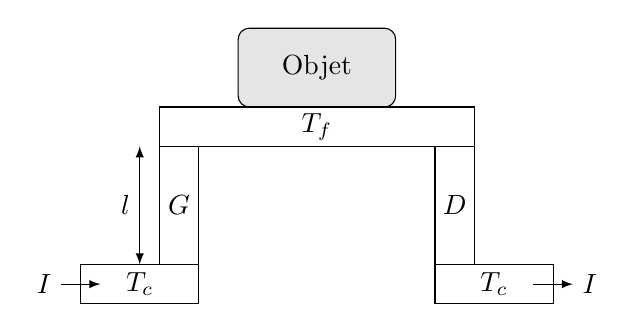
\begin{tikzpicture}
\fill[rounded corners, opacity=0.1, draw opacity=1, draw=black] (0,0) rectangle (2,1);
\draw (-1,-0.5) rectangle (3,0);
\draw (-1,-0.5) rectangle (-0.5,-2);
\draw (3,-0.5) rectangle (2.5,-2);
\draw (-0.5,-2) rectangle (-2,-2.5);
\draw (2.5,-2) rectangle (4,-2.5);

\node at (1,-0.25) {$T_f$};
\node at (-1.25,-2.25) {$T_c$};
\node at (3.25,-2.25) {$T_c$};

\node at (-0.75,-1.25) {$G$};
\node at (2.75,-1.25) {$D$};

\draw[<->,>=latex] (-1.25,-2) -- ++(0,1.5) node[midway, left] {$l$};
\draw[->,>=latex] (-2.25,-2.25) node[left] {$I$} -- ++(0.5,0);
\draw[->,>=latex] (3.75,-2.25) -- ++(0.5,0) node[right] {$I$};

\node at (1,0.5) {Objet};

\end{tikzpicture}
%\caption{Montage pour réfrigération Peltier. L'objet à refroidir est en équilibre thermique avec le conducteur métallique «froid» uniforme à la température $T_f$, lui-même en contact avec deux barreaux de longueur $l$ et de section $S$, le gauche $G$ et le droit $D$. Enfin chacun des barreaux est en contact avec un conducteur métallique «chaud» uniforme à la température $T_c$. L'ensemble est isolé de l'environnement. Un courant électrique $I$ parcourt les barreaux de la gauche vers la droite.}
%\label{fig:peltier}
\end{center}
%\end{figure}
L'objectif de cet exercice est de déterminer la température minimale $T_f^0$ que peut atteindre l'objet.

\begin{quest}
	\item On considère le problème intermédiaire suivant: une barre métallique de section $S$, de conductivité électrique $\sigma$, de coefficient de Fourier $\lambda$, de longueur $l$ et d'axe $Ox$ a pour température $T_C$ en $x=0$ et $T_f$ en $x=l$. Elle est parcourue par un courant d'intensité $I$ constant et uniforme dans la direction des $x$ croissants. Déterminer le profil de température en régime stationnaire (il n'y a pas ici d'effet Peltier).
	\item On suppose que les barreaux ont même dimension, même conductivité électrique $\sigma$ et même coefficient de Fourier $\lambda$ mais des coefficients thermoélectriques différents $\epsilon_G$ et $\epsilon_D$. Déterminer la température $T_f(I)$ en régime stationnaire. Celle-ci dépend également de $T_c$ et des paramètres du problème. Pour ce faire on admettra que le profil de température dans les deux barreaux est le même que celui déterminé en question $1$.
	\item Pour quelle intensité $I_0$ la température de l'objet est-elle minimale? Calculer numériquement $I_0$ et $T_f^0$ pour des barreaux de résistance $R= 4 \cdot 10^{-3} ~\Omega$ avec $\lambda = \SI{1,2}{W.m^{-1}.K^{-1}}$, $S/l= 5$ mm, $\epsilon_D-\epsilon_G= \SI{0,5}{mV.K^{-1}}$ et $T_c=20~\degres$C.
\end{quest}
\end{exo}
%%%%%%%%%%%%%%%%%%%%%%%%%%%%%%%%%%%%%%%%%%%%%%%%%

%%%%%%%%%%%%%%%%%%%%%%%%%%%%%%%%%%%%%%%%%%%%%%%%%%
\begin{exo}[PSI][1]{Transfert thermique dans une coquille sphérique}
On considère un matériau conducteur homogène compris entre deux sphères de centre $O$, de rayons $R_1$ et $R_2$ avec $R_1 < R_2$, de conductivité thermique $\lambda$ constante, de masse volumique $\rho$ et de capacité calorifique massique à pression constante $c_p$. Les parois sphériques de ce matériau sont maintenues constantes à la température $T_1$ en $r = R_1$ et $T_2$ en $r = R_2$, où $r$ est le rayon à partir du centre $O$. Le régime est stationnaire et la transformation est isobare. Le but de l'exercice est de déterminer le flux transféré de l'intérieur vers l'extérieur de la coquille sphérique en présence d'une source volumique d'énergie.
\begin{quest}
	\item Pour commencer, on suppose qu'il n'y a pas de terme source. Montrer que l'on a conservation du flux thermique $\Phi(r) = \int_{\mathcal{S}(r)} \vec{j}_{th} \cdot \vec{\mathrm{d}S}$ à travers le sphère $\mathcal{S}(r)$ de rayon $r$. En déduire la résistance thermique $R_{th}$ en fonction de $\lambda$, $R_1$ et $R_2$. Étudier le cas particulier où
$R_1$ et $R_2$ sont très proches, \emph{i.e.} lorsque $e=R_2-R_1 \ll R_2$.
	\item On suppose à présent l'existence d'un terme source $q$. Entre deux sphères de rayons $r$ et $r+\mathrm{d}r$, l'enthalpie produite par unité de temps est donc $4 \pi r^2 \rho q \mathrm{d}r$. Établir une équation différentielle sur la température $T(r)$ puis la résoudre en s'aidant des conditions aux limites.
	\item Calculer les flux $\Phi(R_1)$ et $\Phi(R_2)$ pour $R_1 = R$ et $R_2 = R + e$ avec $e \ll R$.
\end{quest}
\end{exo}
%%%%%%%%%%%%%%%%%%%%%%%%%%%%%%%%%%%%%%%%%%%%%%%%%%


%%%%%%%%%%%%%%%%%%%%%%%%%%%%%%%%%%%%%%%%%%%%%%%%%%%%%%%%%%%%%%%%%%%%%%%%%
\begin{exo}[PC][3][TD]{Ailette de refroidissement}
Une ailette de refroidissement, modélisée par une tige en cuivre cylindrique homogène d'axe~$(Ox)$, semi-infinie,  de rayon $a=\SI{2}{mm}$, et de conductivité thermique $\lambda = \SI{390}{W.m^{-1}.K^{-1}}$, est au contact d'un processeur de température $T_0=\SI{60}{\dC}$ à son extrémité $x=0$. Sa surface latérale est au contact de l'air à la température $T_{\rm{a}}=\SI{30}{\dC}$. On se place en régime permanent et on suppose que la température $T(x)$ de l'ailette est uniforme le long d'une section, et donc ne dépend que de $x$. On note $h=\SI{60}{W.m^{-2}.K^{-1}}$ le coefficient conducto-convectif.
%La tige présente, au niveau de sa surface en contact avec le fluide, des pertes thermiques par unité de temps et de surface égales à $h(T(x)-T_{\rm{e}})$ si $T(x)$ désigne la température du point de la surface considérée.

Déterminer le profil de température $T(x)$, la puissance thermique dissipée $\mc{P}$, et l'efficacité énergétique $e$ de cette ailette de refroidissement.

\sol{
\begin{center}

\includegraphics[scale=0.3]{ailette.png}
\end{center}
\begin{enumerate}
\item Bilan thermique en régime permanent. Soit $\Vec{j_q}=j_q(x) \ex$ le vecteur densité de flux thermique. Considérons un tronçon élémentaire de matériau de longueur $\d x$, de section $S=\pi a^2$ et de surface latérale $\d S_{\rm lat} = 2\pi a \d x$.  En régime permanent,
$$
0 = \d U = \delta Q = \d \Phi (x) \d t - \d \Phi (x+\d x) \d t - h \d S_{\rm lat} (T(x)-T_a) \d t.
$$
\item Loi de Fourier.
 \begin{multline*}
j_q(x)S\d t-j_q(x+\d x)S\d t - h \times (2\pi a \d x)\times (T(x)-T_a)\d t =  0\\
= -\pi a^2 \d t\lambda\left(\dd{T}{x}(x)-\dd{T}{x}(x+\d x)\right) -  2h\pi a \d x (T(x)-T_0)\\
= \pi a^2 \d t \d x \lambda \ddm{T}{x}{2} -  2h\pi a \d x (T(x)-T_0).
\end{multline*}
On aboutit à l'équation différentielle
\eqbox[*]{ \ddm{T}{x}{2}  - \frac{2h}{\lambda a}(T(x)-T_0) = 0. }
On voit apparaître une distance caractéristique $\delta=\sqrt{\frac{a \lambda}{2h}} = \SI{81}{mm}$.
\item Conditions aux limites.

La solution est de la forme $T(x) = T_a + A e^{-x/\delta} + B e^{x/\delta}$. Dans l'hypothèse où la longueur $L$ de la tige est $L\ll \delta$, on peut la supposer semi-infinie. Alors $B=0$ pour éviter que $T$ ne diverge. Puis le thermostat impose $T(x=0) = A +T_a = T_0$. En conclusion,
\eqbox[*]{T(x) = (T_0-T_a)  e^{-x/\delta} + T_a.}

\item Puissance dissipée.

Le flux thermique dissipé par le tronçon élémentaire vaut
$$
\d \Phi = h \d S_{\rm lat} (T(x)-T_a) =  2\pi a h (T_0-T_a)  e^{-x/\delta} \d x .
$$
La puissance totale dissipée $\mc{P}$ s'obtient par intégration.
$$
\mc{P} = \int \d \Phi = 2\pi a h (T_0-T_a) \int_0^\infty e^{-x/\delta} \d x . %=  2\pi a h (T_0-T_a) \delta = a \sqrt{2 a \lambda h} (T_0-T_a).
$$
On en déduit
\eqbox[*]{\mc{P} =  2\pi a h \delta (T_0-T_a) = \SI{1.8}{W}.}
On remarque que $\mc{P} = \Phi(x=0) = -\lambda \dd{T}{x}(x=0) = \frac{\lambda(T_0-T_a)}{\delta}$ en accord avec la conservation de l'énergie.
\item Efficacité. L'efficacité est le rapport de l'énergie, ou du flux, évacué par l'ailette ($\mc{P}$) sur le flux qui serait évacué sans l'ailette, c'est-à-dire par conducto-convection.
$$
\mc{P}_{\rm cc} = \Phi_{cc}(x=0) = h S (T(x=0)-T_a) = h \pi a^2 (T_0-T_a)
$$
En en déduit
$$
e = \frac{\mc{P}}{\mc{P}_{cc}} = \frac{2\pi a h \delta (T_0-T_a) }{h \pi a^2 (T_0-T_a)} = \frac{2 \delta}{a},
$$
Soit
\eqbox[*]{e = \sqrt{\frac{2\lambda}{h a}} = \SI{81}{}.}
\end{enumerate}

}
\end{exo}
%%%%%%%%%%%%%%%%%%%%%%%%%%%%%%%%%%%%%%%%%%%%%%%%%%%%%%%%%%%%%%%%%%%%%%%%%

%%%%%%%%%%%%%%%%%%%%%%%%%%%%%%%%%%%%%%%%%%%%%%%%%%%%%%%%%%%%%%%%%%%%%%%%%
\begin{exo}[PC][1][devoir]{Fonctionnement d'une ailette de refroidissement}%{3}
Une ailette de refroidissement, modélisée par une tige en cuivre cylindrique homogène d'axe~$(Ox)$, de longueur $L$, de rayon $a=\SI{2}{mm}$,
et de conductivité thermique $\lambda = \SI{390}{W.m^{-1}.K^{-1}}$ %, de capacité calorifique massique $c$, et de masse volumique $\rho$,
est au contact d'un processeur de température $T_0=\SI{60}{\dC}$
à son extrémité $x=0$. La surface de l'ailette est au contact de l'air à la température $T_{\rm{e}}=\SI{30}{\dC}$.  On étudie le régime permanent de l'ailette.


%La tige présente, au niveau de sa surface en contact avec le fluide, des pertes thermiques par unité de temps et de surface égales à $h(T(x)-T_{\rm{e}})$ si $T(x)$ désigne la température du point de la surface considérée.
\begin{fig}
  
\includegraphics[width=7cm]{ailette_cylindre.jpg}
\end{fig}

\subsection{Profil en l'absence de convection}
On néglige pour commencer la conducto-convection au niveau de la surface de contact de l'ailette avec l'air ambiant.
\begin{quest}
\item Justifier que la température dans l'ailette $T(x)$ ne dépend que de l'abscisse $x$.
En déduire que la densité de courant thermique de conduction dans l'ailette est de la forme $\Vec{\jth} = \jth(x) \ex$.

\sol{
Loi de Fourier $\Vec{\jth} = -\lambda \grad T = - \lambda \dd{T}{x} \ex$.
}
\item On considère un tronçon d'ailette de section $S=\pi a^2$ situé entre les abscisses $x$ et $x + \d x$.
En régime permanent, que vaut la variation d'énergie interne $\d U$ de ce tronçon entre deux instants voisins $t$ et $t + \d t$ ?
\sol{
$\d U = 0$ car régime permanent.
}
\item Montrer que le transfert thermique $\delta Q$ reçu par ce tronçon a pour expression
$$
\delta Q = - \dr{\jth}{x}(x) S \d x \d t.
$$
En déduire une équation différentielle simple sur la fonction $T(x)$. Cette équation est-elle en accord avec l'équation de la diffusion thermique ?
\sol{
$\delta Q = \delta \Phi(x) \d t - \delta \Phi(x+\d x)\d t = - (\jth(x)-\jth(x+\d x))S\d t$ car $\Vec{\jth}$ uniforme sur la section. Donc
$$
\delta Q = - \dr{\jth}{x}(x) S \d x \d t.
$$
1er principe : $\delta Q = \d U  = 0$ et donc
$$
0 = \dd{\jth}{x} = -\lambda \ddm{T}{x}{2} \Rightarrow \ddm{T}{x}{2} = 0.
$$
Cohérent avec l'équation de diffusion avec $\dr{T}{t} = 0$ et $T(x)$ fonction de $x$ uniquement.
}
\item Montrer qu'une solution de cette équation est de la forme
$$
  T(x) = A x + B,
$$
avec $A$ et $B$ deux constantes. Déterminer $A$ et $B$ à partir des conditions aux limites, en supposant que l'air ambiant impose la température $T_e$ à l'extrémité $x=L$ de l'ailette.
\sol{
$T(x) =  Ax + B$ avec $T(0) = T_0$ et $T(L) = T_e$ donc $T(x) = (T_e-T_0)\frac{x}{L} + T_0$.
}
\item Calculer le flux thermique $\Phi(x)$ à travers une section $S$ de l'ailette à l'abscisse $x$. Le flux dépend-il de $x$ ? Commenter. Calculer numériquement $\Phi$.
\sol{
$\Phi(x) = -\lambda S \dd{T}{x} = \frac{\lambda S }{L} (T_0-T_e) >0$ car l'énergie passe du processeur en $x=0$ à l'air en $x=L$. Indépendant de $x$ : cohérent avec régime stationnaire et absence le terme de création.
}
\end{quest}

\subsection{Profil en présence de convection}
On prend maintenant en compte la conducto-convection au niveau de la surface latérale de l'ailette.
Les échanges conducto-convectifs vérifient la loi de Newton $\Vec{\jmath}_{\rm cc} = h(T(x)-T_e)\er$, où l'on note $h=\SI{60}{W.m^{-2}.K^{-1}}$ le coefficient conducto-convectif,
et où $\er$ désigne le vecteur unitaire normal, localement, à la surface latérale de l'ailette, et pointant vers l'extérieur.

\begin{quest}
\item On considère à nouveau un tronçon d'ailette de section $S=\pi a^2$ situé entre les abscisses $x$ et $x + \d x$, étudié entre deux instants voisins $t$ et $t + \d t$.
Déterminer la surface latérale $\d S_{\rm lat}$ de ce tronçon, puis le flux thermique de conducto-convection $\d \Phi_{\rm cc}$ perdue par ce tronçon par conducto-convection.
Représenter un schéma de ce tronçon, en faisant apparaître l'ensemble des flux thermiques, y compris les flux de conduction.
\sol{
$\d S_{\rm lat} = 2\pi a \d x$ puis $\d \Phi_{\rm cc} = h \d S_{\rm lat} (T(x)-T_e)$.
}
\item Montrer que le transfert thermique $\delta Q$ reçu par ce tronçon a pour expression
$$
\delta Q = - \dr{\jth}{x}(x) \pi a^2 \d x \d t - 2\pi a h  (T(x)-T_e) \d x \d t.
$$
\sol{
Bilan thermique en régime permanent. Soit $\Vec{j_q}=j_q(x) \ex$ le vecteur densité de flux thermique. Considérons un tronçon élémentaire de matériau de longueur $\d x$, de section $S=\pi a^2$ et de surface latérale $\d S_{\rm lat} = 2\pi a \d x$.  En régime permanent,
$$
0 = \d U = \delta Q = \d \Phi (x) \d t - \d \Phi (x+\d x) \d t - h \d S_{\rm lat} (T(x)-T_a) \d t.
$$
Loi de Fourier.
 \begin{multline*}
j_q(x)S\d t-j_q(x+\d x)S\d t - h \times (2\pi a \d x)\times (T(x)-T_a)\d t =  0\\
= -\pi a^2 \d t\lambda\left(\dd{T}{x}(x)-\dd{T}{x}(x+\d x)\right) -  2h\pi a \d x (T(x)-T_0)\\
= \pi a^2 \d t \d x \lambda \ddm{T}{x}{2} -  2h\pi a \d x (T(x)-T_0).
\end{multline*}
}
\item En déduire l'équation vérifiée par la température en régime permanent,
\begin{equation}\label{eq:T}
   \ddm{T}{x}{2}  = \frac{T(x)-T_e}{\delta^2},
\end{equation}
où l'on donnera l'expression et la dimension de $\delta$. Application numérique ?
\sol{
On trouve $0 = \delta Q = \pi a^2 \d t \d x \lambda \ddm{T}{x}{2} -  2h\pi a \d x (T(x)-T_e)$.
On voit apparaître une distance caractéristique $\delta=\sqrt{\frac{a \lambda}{2h}} = \SI{81}{mm}$.
}
\item
On suppose que le processeur de température $T_0$ joue le rôle de thermostat, et on prend en compte la conducto-convection à l'extrémité libre de l'ailette.
 Quelles conditions aux limites vérifie l'ailette en $x=0$ et en $x=L$ ?
 \sol{
 Continuité de la température en $x=0$, soit $T(x=0) = T_0$.
 Continuité de la densité de courant thermique en $x=L$, soit $-\lambda \dd{T}{x}(x=L) = h(T(L)-T_e)$.
 }
 \item Donner la solution générale de l'\Eq{T}, en faisant apparaître deux constantes $A$ et $B$.
 Comment se simplifie la condition aux limites en $x=L$ si $L \gg \delta$ ? En déduire $A$ et $B$ et l'expression de $T(x)$.
 \sol{
 On trouve $T(x) = A \exp(+x/\delta) + B \exp(-x/\delta) + T_e$. Les conditions aux limites donnent
 $T_0 = A + B + T_e$ et $-\lambda (A\exp(L/\delta)-B\exp(-L/\delta))/\delta  = h(T(L)-T_e)=0$ si $L \gg \delta$ avec $A=0$.
 }
\end{quest}

\subsection{Efficacité de l'ailette}

\begin{quest}
\item Montrer que la puissance totale $\mc{P}_a$ perdue par l'ailette par conducto-convection au niveau de sa paroi latérale s'écrit pour $L \gg \delta$,
\begin{equation}
  \mc{P}_a = 2\pi a h \delta (T_0-T_e).
\end{equation}
Application numérique ?
\sol{
$\mc{P}_a = \SI{1.83}{W}$
}
\item Le processeur libère une puissance $\mc{P}= \SI{200}{W}$. Combien faut-il d'ailettes pour maintenir le processeur à la température $T_0 = \SI{60}{\dC}$ en régime stationnaire ?
\sol{
Il en faut au moins $N=\mc{P}/\mc{P}_a = 110$.
}
\end{quest}
%On se place en régime permanent et on suppose que la température $T(x)$ de l'ailette est uniforme le long d'une section, et donc ne dépend que de $x$.
\end{exo}
%%%%%%%%%%%%%%%%%%%%%%%%%%%%%%%%%%%%%%%%%%%%%%%%%%%%%%%%%%%%%%%%%%%%%%%%%



%%%%%%%%%%%%%%%%%%%%%%%%%%%%%%%%%%%%%%%%%%%%%%%%%%%%%%%%%%%%%%%%%%%%%%%%%
\begin{exo}[PC][3][TD]{Principe d'une ailette de refroidissement}%{3}
  \Notions{\item Conduction thermique \task Conducto-convection \item Régime permanent}
  \Annale[Physique TPC]{CCINP}{2018}
Une ailette de refroidissement, modélisée par une tige en cuivre cylindrique homogène d'axe~$(Ox)$, de longueur $L$, de rayon $a=\SI{2}{mm}$,
et de conductivité thermique $\lambda = \SI{390}{W.m^{-1}.K^{-1}}$ %, de capacité calorifique massique $c$, et de masse volumique $\rho$,
est au contact d'un processeur de température $T_0=\SI{60}{\dC}$
à son extrémité $x=0$. La surface de l'ailette est au contact de l'air à la température $T_{\rm{e}}=\SI{30}{\dC}$. On étudie le régime permanent de l'ailette.


%La tige présente, au niveau de sa surface en contact avec le fluide, des pertes thermiques par unité de temps et de surface égales à $h(T(x)-T_{\rm{e}})$ si $T(x)$ désigne la température du point de la surface considérée.
% \begin{fig}
%   
\includegraphics[width=7cm]{ailette_cylindre.jpg}
% \end{fig}

On prend en compte la conducto-convection au niveau de la surface latérale de l'ailette.
On considère un tronçon élémentaire d'ailette de section $S=\pi a^2$ situé entre les abscisses $x$ et $x + \d x$, étudié entre deux instants voisins $t$ et $t + \d t$. Les échanges conducto-convectifs vérifient la loi de Newton, ce qui implique que le flux thermique de conducto-convection $\d \Phi_{\rm cc}$ perdue par ce tronçon par conducto-convection a pour expression $\d \Phi_{\rm cc} = \d S_{\rm lat} h(T(x)-T_e)$, où $ \d S_{\rm lat}$ désigne la surface latérale du tronçon.

\begin{quest}
\item Montrer que le transfert thermique $\delta Q$ reçu par ce tronçon a pour expression
$$
\delta Q = - \dr{\jth}{x}(x) \pi a^2 \d x \d t - 2\pi a h  (T(x)-T_e) \d x \d t.
$$
\sol{
$\d S_{\rm lat} = 2\pi a \d x$ puis $\d \Phi_{\rm cc} = h \d S_{\rm lat} (T(x)-T_e)$.
Bilan thermique en régime permanent. Soit $\Vec{j_q}=j_q(x) \ex$ le vecteur densité de flux thermique. Considérons un tronçon élémentaire de matériau de longueur $\d x$, de section $S=\pi a^2$ et de surface latérale $\d S_{\rm lat} = 2\pi a \d x$.  En régime permanent,
$$
0 = \d U = \delta Q = \d \Phi (x) \d t - \d \Phi (x+\d x) \d t - h \d S_{\rm lat} (T(x)-T_a) \d t.
$$
Loi de Fourier.
 \begin{multline*}
j_q(x)S\d t-j_q(x+\d x)S\d t - h \times (2\pi a \d x)\times (T(x)-T_a)\d t =  0\\
= -\pi a^2 \d t\lambda\left(\dd{T}{x}(x)-\dd{T}{x}(x+\d x)\right) -  2h\pi a \d x (T(x)-T_0)\\
= \pi a^2 \d t \d x \lambda \ddm{T}{x}{2} -  2h\pi a \d x (T(x)-T_0).
\end{multline*}
}
\item En déduire l'équation vérifiée par la température en régime permanent,
\begin{equation}\label{eq:T}
   \ddm{T}{x}{2}  = \frac{T(x)-T_e}{\delta^2},
\end{equation}
où l'on donnera l'expression et la dimension de $\delta$. Application numérique ?
\sol{
On trouve $0 = \delta Q = \pi a^2 \d t \d x \lambda \ddm{T}{x}{2} -  2h\pi a \d x (T(x)-T_e)$.
On voit apparaître une distance caractéristique $\delta=\sqrt{\frac{a \lambda}{2h}} = \SI{81}{mm}$.
}
\item
On suppose que le processeur de température $T_0$ joue le rôle de thermostat, et on prend en compte la conducto-convection à l'extrémité libre de l'ailette.
 Quelles conditions aux limites vérifie l'ailette en $x=0$ et en $x=L$ ?
 \sol{
 Continuité de la température en $x=0$, soit $T(x=0) = T_0$.
 Continuité de la densité de courant thermique en $x=L$, soit $-\lambda \dd{T}{x}(x=L) = h(T(L)-T_e)$.
 }
 \item Donner la solution générale de l'\Eq{T}, en faisant apparaître deux constantes $A$ et $B$.
 Comment se simplifie la condition aux limites en $x=L$ si $L \gg \delta$ ? En déduire $A$ et $B$ et l'expression de $T(x)$.
 \sol{
 On trouve $T(x) = A \exp(+x/\delta) + B \exp(-x/\delta) + T_e$. Les conditions aux limites donnent
 $T_0 = A + B + T_e$ et $-\lambda (A\exp(L/\delta)-B\exp(-L/\delta))/\delta  = h(T(L)-T_e)=0$ si $L \gg \delta$ avec $A=0$.
 }
% \end{quest}

% \subsection{Efficacité de l'ailette}

% \begin{quest}
\item Montrer que la puissance totale $\mc{P}_a$ perdue par l'ailette par conducto-convection au niveau de sa paroi latérale s'écrit pour $L \gg \delta$,
\begin{equation}
  \mc{P}_a = 2\pi a h \delta (T_0-T_e).
\end{equation}
Application numérique ?
\sol{
$\mc{P}_a = \SI{1.83}{W}$
}
\item Le processeur libère une puissance totale $\mc{P}= \SI{200}{W}$. Combien faut-il d'ailettes pour maintenir le processeur à la température $T_0 = \SI{60}{\dC}$ en régime stationnaire ?
\sol{
Il en faut au moins $N=\mc{P}/\mc{P}_a = 110$.
}
\end{quest}
%On se place en régime permanent et on suppose que la température $T(x)$ de l'ailette est uniforme le long d'une section, et donc ne dépend que de $x$.
\end{exo}
%%%%%%%%%%%%%%%%%%%%%%%%%%%%%%%%%%%%%%%%%%%%%%%%%%%%%%%%%%%%%%%%%%%%%%%%%


%%%%%%%%%%%%%%%%%%%%%%%%%%%%%%%%%%%
\begin{exo}[PC][1][TD]{Isolation thermique d'un bâtiment}
  On souhaite étudier l'isolation thermique d'un bâtiment rectangulaire entourée de quatre murs. Les murs sont en béton de conductivité thermique $\lambda = \SI{1.75}{W.m^{-1}.K^{-1}}$, sont d'épaisseur $e=\SI{10}{cm}$ et couvrent une surface totale $S=\SI{80}{m^2}$.
   % 'ensemble des quatre murs a une résistance thermique $R_{\rm m} = \SI{}{}$.
   \begin{quest}
     \item  Calculer la résistance thermique $R_{\rm m}$ de l'ensemble des murs du bâtiment.
     \sol{
     Revoir cours pour démonstration de la résistance thermique d’un plan de surface $S$ et d’épaisseur $e$. Pour quatre murs de surface totale $S$, on trouve une résistance thermique 
     \eqbox{
     R_{\rm m} = \frac{e}{\lambda S} =\SI{7.1e-4}{K.W^{-1}}
     }
     }
     \item On isole les murs avec une couche de laine minérale de même épaisseur $e$ et de conductivité thermique $\SI{0.045}{W.m^{-1}.K^{-1}}$. Les murs et l'isolant sont-ils associés en série ou en parallèle ? Calculer la résistance thermique $R_{\rm \ell}$ de la couche de laine minérale et la résistance thermique totale $R_{\rm i}$ des murs isolés.
     \sol{
     Les murs et la laine de verre sont disposés en \udl{série}. En effet, la couche de laine tapisse entièrement l’intérieur des murs, ce qui implique que le béton et la laine sont soumises au même flux thermique. Les résistances thermiques s’additionnent :
     \eqbox{
       R_{\rm i} = R_{\rm m} + R_{\rm \ell} = \SI{2.7e-2}{K.W^{-1}}.
     }
     La résistance thermique est dominée par celle de la laine isolante.
     }
     \item On ajoute une fenêtre de mauvaise qualité dans le mur de résistance thermique $R_{\rm f} = \SI{5e-4}{K.W^{-1}}$. Les murs isolés et la fenêtre sont-ils associés en série ou en parallèle ? Calculer la résistance totale $R_{\rm b}$ du bâtiment et commenter.
     \sol{
     La fenêtre et les murs sont soumis à la même différnce de température : ils sont donc disposés en \udl{parallèle}. Les conductances thermiques s’additionnent.
    %  \eqbox{
      $$
       \frac{1}{R_{\rm b}} =    \frac{1}{R_{\rm i}} + \frac{1}{R_{\rm f}} \Rar \boxed{R_{\rm b} = \frac{R_{\rm i} R_{\rm f}}{R_{\rm i} + R_{\rm f}} = \SI{5e-4}{K.W^{-1}}.
       %  }
       }
       $$
       La résistance thermique est dominée par la fenêtre, qui occasionne d’importcantes pertes.
     }
   \end{quest}
\end{exo}
%%%%%%%%%%%%%%%%%%%%%%%%%%%%%%%%%%%

%%%%%%%%%%%%%%%%%%%%%%%%%%%%%%%%%%%%%%%%%%%%%%%%%%%%%%%%%%%%%%%%%%%%%%%%%
\begin{exo}[PC][3][python]{Résolution numérique de l’équation de diffusion thermique}
  \Notions{\item Équation de diffusion \task  Méthode des différences finies \task  Régime transitoire}
L’objectif de cet exercice est de résoudre numériquement l’équation de la diffusion thermique dans une situation simple. On se place à une dimension d’espace, de sorte que la température $T(x,t)$ vérifie
\begin{equation}\label{eq:diffu_python}
\dr{T}{t} = \kappa \drm{T}{x}{2}.
\end{equation}
On considère une barre de cuivre de longueur $L$ dont les extrémités ont portés à la température de la glace fondante $T_g = \SI{0}{\dC}$ : on impose donc les conditions aux limites $T(x=0,t) = T(x=L,t) = T_g$ à tout instant $t$. On prend comme condition initiale $T(x,t=0) = T_0 \sin(2\pi x)$ avec $T_0 = \SI{20}{\dC}$.
On se reportera pour la suite à l'énoncé de l'exercice du TD Physique Python sur capytale :
\begin{center}
  \url{https://capytale2.ac-paris.fr/p/basthon/n/?kernel=python3&id=1765716}.
\end{center}
\begin{remarque}
  On pourra aussi s'aider du TD Physique Python d'introduction aux tableaux \texttt{numpy.array} : \url{https://capytale2.ac-paris.fr/p/basthon/n/?kernel=python3&id=1761691}.
\end{remarque}

% Comme pour toute résolution numérique, il nous faut discrétiser le problème pour chercher une solution approchée. On introduit $\d x$ et $\d t$ les pas d’espace et de temps. Soit $T_j^i=T(x,t)$ la température au point $x=j\d x$ à l’instant $t=i\d t$.
%
% \begin{quest}
% \item Effectuer un développement limité de $T(x,t+\d t )$ à l’ordre $1$ en $\d t$. En déduire une expression approchée de $\dr{T}{t}(x,t)$ en fonction de $T_j^n$ et $T_j^{n+1}$.
%
% \sol{
% L’approximation linéaire donne
% $ T(x,t+ \d t ) = T(x,t) + \dr{T}{t}(x,t) \d t + O(\d t^2)$, soit $T^{n+1}_j \simeq T_j^n + \dr{T}{t}(x,t) \d t$ et
% $$
%  \dr{T}{t}(x,t) \simeq  \frac{T^{n+1}_j - T_j^n}{\d t}.
% $$
% }
%
% \item Effectuer un développement limité de $T(x+\d x,t)$ et $T(x-\d x,t)$ à l’ordre deux en $\d x$. En déduire une expression approchée de $\drm{T}{x}{2}(x,t)$. Comment calculer l’incrément de température $\d T$ entre les étapes $n$ et $n+1$ à partir de $T_{j-1}^n$, $T_{j}^n$ et  $T_{j+1}^n$ ?
%
% \emph{Cette méthode de calcul approché de dérivées se nomme méthode des différences finies.}
%
% \sol{
% On a d’une part
% $T(x+\d x,t) \simeq T(x,t) + \d x \dd{T}{x}(x,t) + \frac{\d x^2}{2}\drm{T}{x}{2}(x,t)$ et
% $T(x-\d x,t) \simeq T(x,t) - \d x \dd{T}{x}(x,t) + \frac{\d x^2}{2}\drm{T}{x}{2}(x,t)$. En sommant les deux développements, il vient
% $$
% T(x+\d x,t) + T(x-\d x,t) \simeq 2 T(x,t)  + \d x^2 \drm{T}{x}{2}(x,t)\quad \Rightarrow \quad \drm{T}{x}{2}(x,t) \simeq  \frac{T_{j+1}^n + T_{j-1}^n - 2 T_j^n}{\d x^2}.
% $$
% On trouve l’incrément de température
% $$
% \d T =  T^{n+1}_j - T_j^n \simeq \d t \dr{T}{t}(x,t) = \kappa \d t \drm{T}{x}{2}(x,t) \simeq \frac{\kappa \d t }{\d x^2}(T_{j+1}^n + T_{j-1}^n - 2 T_j^n).
% $$
% }
%
% \item On suppose avoir défini
% %une variable $\rm{NT}$ (au nombre de pas de temps), et
% une variable $\rm{NX}$ (nombre de pas d’espace). On souhaite définir le tableau des pas d’espace $\rm{x}$, le tableau des températures initiales $\rm{T}$, et un tableau $\rm{d T}$ de taille $\rm{NX}$ rempli de zéros. Comment implémenter ces définitions avec la bibliothèque \texttt{numpy} de \texttt{python} ?
%
% \sol{
% \inputminted{python}{def_tableaux.py}
% }
%
% \item On suppose avoir en plus défini les variables $\rm{dt}$, $\rm{dx}$, et $\rm{K}$ (diffusivité thermique). Proposer un programme \texttt{python} pour résoudre l’équation de diffusion.
%
% \sol{
% \inputminted{python}{algo_resolution.py}
% }
% \end{quest}
\end{exo}
%%%%%%%%%%%%%%%%%%%%%%%%%%%%%%%%%%%%%%%%%%%%%%%%%%%%%%%%%%%%%%%%%%%%%%%%%


%%%%%%%%%%%%%%%%%%%%%%%%%%%%%%%%%%%
\begin{exo}[PC][1][devoir]{Méthode d'Euler et équation de diffusion}
\setcounter{subsection}{0}

On s'intéresse ici à une barre métallique cylindrique dont la surface latérale est calorifugée. Les deux extrémités gauche et droite de la barre sont en contact avec de la glace fondante de température $T_g = \SI{0}{\degree C}$, qui joue le rôle de thermostat.  L’objectif de cet exercice est de résoudre numériquement l’équation de la diffusion thermique dans cette situation simple. On appelle désormais $L=\SI{1}{m}$ la longueur de la barre. On rappelle que l'équation de diffusion thermique s'écrit
$$
\frac{\partial T}{\partial t} = \kappa \frac{\partial^2 T}{\partial x^2},
$$
où $\kappa$ désigne la diffusivité thermique. On considérera un matériau de diffusivité $\kappa=\SI{e-4}{m^2.s^{-1}}$.


% \subsection{Etude numérique}

% \subsection{Modélisation}

Nous allons dans la suite déterminer la température $T(x,t)$, en tout point $x$ de la barre,
 et à tout instant $t$ de l'expérience. Pour cela, nous allons découper la barre en tronçons de longueur $\d x=\SI{1}{cm}$.
L'étude sera menée sur une durée de $\Delta t = \SI{30}{min}$, avec un pas temporel de $\d t=\SI{0,4}{s}$. La fonction $T(x,t)$ sera donc approximée par un tableau \texttt{T[i,j]} de telle sorte que :

$$T[i,j] = T(x=j dx,t=i dt).$$

Autrement dit, chaque ligne \texttt{i} du tableau correspond à l'instant $t=i\mathrm{d}t$ de l'expérience (la ligne \texttt{i=0} correspondant à l'instant initial), et chaque colonne \texttt{j} du tableau représente la position $x=j\mathrm{d}x$ (la colonne \texttt{j=0} correspondant au bord gauche).

Le tableau utilisé est de type \texttt{numpy.array}. On aura de plus besoin du module \texttt{matplotlib.pyplot} pour effectuer les représentations graphiques du champ de température. On importe pour cela les modules suivants. 
\begin{minted}{python}
import numpy as np
import matplotlib.pyplot as plt
\end{minted}

\subsection{Initialisation}
\begin{quest}
  \item	

  On nommera désormais les variables entières \texttt{Nt} et \texttt{Nx} correspondant respectivement au nombre de lignes  et de colonnes du tableau \texttt{T}.
  
  Compléter les lignes suivantes pour définir \texttt{Nx} et \texttt{Nt} sur Python, et créer le tableau \texttt{T} en le remplissant de zéros pour l'instant. Créer également les tableaux \texttt{x} et \texttt{t} correspondant respectivement aux positions $x$ et aux instants $t$ pour lesquels la température est évaluée.
  \begin{minted}{python}
dx = 1e-2
dt = 4e-1
L  = 1
Deltat = 30*60
  \end{minted}
% \sol{
    \begin{minted}{python}
Nx = int(L/dx) + 1
Nt = int(Deltat/dt) + 1

T = np.zeros((Nt,Nx))

x = np.array([j*dx for j in range(Nx)])
t = np.array([i*dt for i in range(Nt)])
  \end{minted}
% }
\item On suppose que le profil de température initial a pour expression 
$$
T(x,t=0) = T_0 \sin (2\pi x/L),
$$
avec $T_0 = \SI{20}{\degree C}$. Remplir la première ligne du tableau \texttt{T} pour spécifier les conditions initiales de l'expérience.
% \sol{
  \begin{minted}{python}
T0 = 20
T[0,:] = T0*np.sin(2*np.pi*x/L)
  \end{minted}
% }
\item Compléter le code suivant pour tracer l'évolution de la température initiale au sein de la barre.
\begin{minted}{python}
plt.close()
plt.figure()
plt.grid()
plt.xlabel("x (m)")
plt.ylabel("T (°C)")
plt.title("Profil de température initial")
\end{minted}
% \sol{
\begin{minted}{python}
plt.plot(x,T[0,:])
plt.show()
\end{minted}
% }
\end{quest}


\begin{quest}
  \item	
  Remplir le tableau \texttt{T} de manière à imposer, à tout instant, les conditions aux limites aux deux extrémités de la barre, $T(x=0,t)=0$ et $T(x=L,t)=0$.
  % \sol{
    \begin{minted}{python}
    for i in range (1,Nt): # l'instant initial a déjà été traité
      T[i,0]  = 0
      T[i,-1] = 0
    \end{minted}
    % }
  \end{quest}
  
  \subsection{Discrétisation de l'équation de diffusion}
  Il s'agit donc désormais de résoudre l'équation :
  $$\frac{\partial T}{\partial t} = \kappa \frac{\partial^2 T}{\partial x^2}.$$
  \begin{quest}
    \item En utilisant l'approximation de la dérivée, exprimer $\dfrac{\partial T}{\partial t}(t=i\mathrm{d}t,x=j\mathrm{d}x)$ en fonction de $T[i,j]$ et de $T[i+1,j]$.
    \sol{
      $$\dfrac{\partial T}{\partial t}(t=i\mathrm{d}t,x=j\mathrm{d}x) \simeq \frac{T[i+1,j]-T[i,j]}{dt}$$
    }
    \item Soit une fonction $f$. En écrivant la formule de Taylor à l’ordre 2 pour $f(x+\d x)$ et $f(x-\d x)$, démontrer que : 
    $$ f''(x)\simeq\frac{f(x+\d x)+f(x-\d x)-2f(x)}{\d x^2}.$$
    \item En déduire l'approximation de $\dfrac{\partial^2 T}{\partial x^2}(t=i\mathrm{d}t,x=j\mathrm{d}x)$ en fonction de $T[i,j]$, de $T[i,j+1]$ et de $T[i,j-1]$.
    \sol{
      $$\dfrac{\partial^2 T}{\partial x^2}(t=i\mathrm{d}t,x=j\mathrm{d}x) \simeq \frac{T[i,j+1]+T[i,j-1]-2T[i,j]}{dx^2}.$$
    }
    \item En déduire que la résolution de l'équation de diffusion thermique dans la barre se ramène au schéma numérique :
    \begin{center}
      $$ T[i+1,j]=T[i,j]+\frac{\kappa \mathrm{d}t}{\mathrm{d}x^2} \left( T[i,j+1]+T[i,j-1]-2T[i,j]\right).$$
    \end{center}
  \end{quest}

  \subsection{Résolution}
  On peut montrer qu'un tel schéma numérique converge si $$\frac{\kappa \d t}{\d x^2}<\frac{1}{2}.$$ Avec les valeurs de $\d x$ et de $\d t$ choisies, cette condition est respectée pour la valeur choisie de la diffusivité thermique $\kappa=\SI{e-4}{m^2.s^{-1}}$.
  \begin{quest}
    \item	Implémenter ce schéma numérique en réalisant une boucle sur \texttt{i} et éventuellement sur \texttt{j} pour remplir le tableau \texttt{T} dans son intégralité.
    % \sol{
      \begin{minted}{python}
      kappa = 1e-4

      for i in range(0,Nt-1): # on remplit à l'indice i+1
        for j in range(1,Nx-1): # les conditions aux limites sont déjà fixées
          T[i+1,j]=T[i,j]+kappa*dt/(dx**2)*(T[i,j+1]+T[i,j-1]-2*T[i,j])
    \end{minted}
    % }
    \item On souhaite tracer le profil de température aux différents instants définis dans la liste ci-dessous. Compléter le code ci-dessous de sorte à tracer sur un même graphique légendé l'évolution du profil de température dans le temps.
%     \begin{minted}{python}
%     plt.close()
%     plt.figure()
%     plt.grid()
%     plt.xlabel("x (m)")
%     plt.ylabel("T (°C)")
%     plt.title("Profil de température dans la barre à différents instants")

%     instants = [0,1,3,6,9,12,15,30] # instants choisis en minutes
% \end{minted}
% % \sol{
%   \begin{minted}{python}
%   for t in instants: # tracé du profil du température aux instants choisis
%     i = int(t*60/dt)
%     plt.plot(x,T[i,:],label="t = "+str(t)+" min")
    
% plt.legend()
% plt.show()
% \end{minted}
% }
  \end{quest}
\end{exo}
%%%%%%%%%%%%%%%%%%%%%%%%%%%%%%%%%%%

%%%%%%%%%%%%%%%%%%%%%%%%%%%%%%%%%%%
\begin{exo}[PC][1][devoir]{Thermodynamique d'un réacteur à eau pressurisé}
  
\textsc{Données} :

\begin{center}
  
\begin{tabular}{|c|c|c|c|c|}
  \hline \begin{tabular}{c} 
  Pression de \\
  vapeur \\
  saturante \\
  (bar) \\
  $1 \mathrm{bar}=10^5 \mathrm{~Pa}$
  \end{tabular} & \multicolumn{2}{|c|}{ enthalpies massiques $\left(\mathrm{kJ} \cdot \mathrm{kg}^{-1}\right)$} & \multicolumn{2}{c|}{\begin{tabular}{c} 
  entropies massiques $\left(\mathrm{kJ} . \mathrm{K}^{-1} \cdot \mathrm{~kg}^{-1}\right)$
  \end{tabular}} \\
  \cline { 2 - 5 } & \begin{tabular}{c} 
  à l'état de \\
  liquide saturant : \\
  $h^{\prime}$
  \end{tabular} & \begin{tabular}{c} 
  à l'état de vapeur \\
  saturante : \\
  $h^{\prime \prime}$
  \end{tabular} & \begin{tabular}{c} 
  à l'état de \\
  liquide saturant: \\
  $s^{\prime}$
  \end{tabular} & \begin{tabular}{c} 
  à l'état de vapeur \\
  saturante : \\
  $s^{\prime \prime}$
  \end{tabular} \\
  \hline 0,05 & 137,8 & 2561,6 & 0,4763 & 8,3960 \\
  \hline 10 & 762,6 & 2776,2 & 2,1382 & 6,5828 \\
  \hline 70 & 1267,4 & 2773,5 & 3,1219 & 5,8162 \\
  \hline
  \end{tabular}
\end{center}

% \begin{tabularx}{\textwidth}{|p{5cm}|c|c|c|c|}
% \hline
% \multirow[t]{2}{*}{Pression de vapeur saturante (bar) $1 \mathrm{bar}=10^{5} \mathrm{~Pa}$} & \multicolumn{2}{|l|}{enthalpies massiques $\left(\mathrm{kJ}^{\text {arg }}{ }^{-1}\right.$ )} & \multicolumn{2}{|l|}{entropies massiques $\left(\mathrm{kJ} \cdot \mathrm{K}^{-1} \cdot \mathrm{~kg}^{-1}\right.$ )} \\
% \hline
%  &
% à l'état de 
% liquide saturant : h' 
%  & à l'état de vapeur saturante: $ h^{\prime \prime} $ & à l'état de liquide saturant: $ s^{\prime} $ & à l'état de vapeur saturante : $ s^{\prime \prime} $ \\
% \hline
% 0,05 & 137,8 & 2561,6 & 0,4763 & 8,3960 \\
% \hline
% 10 & 762,6 & 2776,2 & 2,1382 & 6,5828 \\
% \hline
% 70 & 1267,4 & 2773,5 & 3,1219 & 5,8162 \\
% \hline
% \end{tabularx}


On rappelle que l'enthalpie massique $h$ d'un mélange diphasique de titre massique en vapeur $x$ est donnée par la relation: $h=x h^{\prime \prime}+(1-x) h^{\prime}$, où $h^{\prime \prime}$ et $h$ ' sont respectivement les enthalpies massiques à l'état de vapeur saturante et à l'état de liquide saturant. Par ailleurs, l'entropie massique $s$ d'un mélange diphasique de titre $x$ est donnée par la relation : $s=x s^{\prime \prime}+(1-x) s^{\prime}$, où $s^{\prime \prime}$ et $s^{\prime}$ sont respectivement les entropies massiques à l'état de vapeur saturante et à l'état de liquide saturant.

Le circuit secondaire est constitué du générateur de vapeur (G.V.), d'une turbine (T) reliée à un alternateur, d'un condenseur $(\mathrm{C})$ et d'une pompe d'alimentation secondaire $(\mathrm{P})$, comme précisé en figure 1.\\
%%%%%%%%%%%%%%%%%%%%%%%%%%%%%%%%%%%%%%%%%%%
\begin{fig}[label]
\centering

\includegraphics[width=0.7\columnwidth]{2024_11_11_a8e446469c675312293dg-1}
\capt{Circuit secondaire simplifié}
\end{fig}
%%%%%%%%%%%%%%%%%%%%%%%%%%%%%%%%%%%%%%%

Pour l'ensemble du problème, nous négligerons les frottements ainsi que les variations d'énergie cinétique et d'énergie potentielle du fluide secondaire. L'expression du premier principe pour une masse $\boldsymbol{m}=\mathbf{1} \mathbf{k g}$ de fluide en écoulement au travers d'une machine est : $\boldsymbol{\Delta h}=\boldsymbol{w}_{\boldsymbol{i}}+\boldsymbol{q}_{\boldsymbol{e}}$, où $\Delta h$ représente la différence $h_{s}-h_{e}$ entre les enthalpies massiques (en $\mathrm{kJ}^{-1} \mathrm{~kg}^{-1}$ ) du fluide à la sortie $h_{s}$ et à l'entrée $h_{e}$ de la machine, $w_{u}$ le travail massique utile, c'est-à-dire le travail massique (en $\mathrm{kJ} . \mathrm{kg}^{-1}$ ) échangé entre une masse $m=1 \mathrm{~kg}$ de fluide et les parois mobiles de la machine, $q_{e}$ le transfert thermique entre le kilogramme de fluide et la machine (en $\mathrm{kJ}^{-1} \mathrm{~kg}^{-1}$ ). Dans le condenseur et le générateur de vapeur il n'y a pas de pièce mobile.

\subsection{Questions préliminaires}
\begin{quest}
\item Sur un diagramme de Clapeyron \Fig{clapy} que vous reproduirez, préciser la position du point critique, les parties courbes de rosée et d'ébullition. Indiquer également les domaines du liquide, du mélange diphasique et de la vapeur surchauffée. Mentionner où se trouve le liquide saturant et la vapeur saturante.\\
%%%%%%%%%%%%%%%%%%%%%%%%%%%%%%%%%%%%%%%%%%%
\begin{fig}[clapy]
\centering

\includegraphics[width=0.7\columnwidth]{2024_11_11_a8e446469c675312293dg-2}
\capt{Diagramme de Clapeyron.}
\end{fig}
%%%%%%%%%%%%%%%%%%%%%%%%%%%%%%%%%%%%%%%
  \item Sur le diagramme de Clapeyron de la \Fig{iso_clapey}, l'allure de l'isotherme correspondant à la température $T=306 \mathrm{~K}$ a été représentée. Justifier l'allure de cette isotherme pour chaque domaine. On pourra, dans le domaine de la vapeur surchauffée, se référer au modèle du gaz parfait. Tracer l'allure de l'isotherme correspondant à la température $T=559 \mathrm{~K}$ sur un diagramme de Clapeyron que vous reproduirez et où apparaît l'allure de l'isotherme correspondant à la température $T=306 \mathrm{~K}$.\\
  %%%%%%%%%%%%%%%%%%%%%%%%%%%%%%%%%%%%%%%%%%%
  \begin{fig}[iso_clapey]
\centering

\includegraphics[width=0.7\columnwidth]{2024_11_11_a8e446469c675312293dg-2(1)}
\capt{Isotherme dans le diagramme de Clapeyron.}
\end{fig}
%%%%%%%%%%%%%%%%%%%%%%%%%%%%%%%%%%%%%%%

\item Démontrer qu'une transformation adiabatique réversible est une transformation isentropique.

\item En considérant que l'eau liquide dans une pompe est incompressible et de volume massique $v=10^{-3} \mathrm{~m}^{3} \cdot \mathrm{~kg}^{-1}$, calculer le travail massique utile $w_{u \mathrm{P}}$ échangé par l'eau circulant dans une pompe, en considérant la transformation adiabatique réversible et une augmentation de pression de $\Delta P=70$ bar. On rappelle que la variation élémentaire de l'enthalpie massique $d h$ du fluide peut s'écrire: $d h=T  d s+v  d P$.

Ce travail peut être considéré comme négligeable devant les autres échanges énergétiques; dans toute la suite du problème, le travail indiqué échangé par un liquide sera systématiquement considéré comme nul.\\
En déduire alors, que l'enthalpie massique du liquide reste constante lors de son passage dans une pompe.

\subsection{Etude du cycle thermodynamique simplifié}
Le fluide secondaire subit le cycle thermodynamique suivant:

\begin{itemize}
  \item $1 \rightarrow 2$ : détente adiabatique réversible dans la turbine,
  \item $2 \rightarrow 3$ : liquéfaction isobare totale dans le condenseur,
  \item $3 \rightarrow 4$ : compression adiabatique réversible dans la pompe d'alimentation secondaire,
  \item $4 \rightarrow 1$ : échauffement puis vaporisation isobare dans le générateur de vapeur saturante.
\end{itemize}

Le tableau suivant précise l'état thermodynamique du fluide secondaire en certains points du cycle :
\begin{center}
  
  \begin{tabular}{|c|c|c|c|c|c|}
    \hline
    Point & \begin{tabular}{c}
      Pression \\
      (bar) \\
      $1 \mathrm{bar}=10^{5} \mathrm{~Pa}$ \\
    \end{tabular} & \begin{tabular}{c}
      Tempé- \\
      rature \\
      $(\mathrm{K})$ \\
    \end{tabular} & \begin{tabular}{c}
      Etat du fluide \\
      secondaire \\
    \end{tabular} & \begin{tabular}{c}
  Enthalpie \\
  massique \\
  $\left(\mathrm{kJ}^{-1} \mathrm{~kg}^{-1}\right.$ \\
\end{tabular} & \begin{tabular}{c}
  Entropie \\
  massique \\
  $\left(\mathrm{kJ}^{-1} \cdot \mathrm{Kg}^{-1}\right)$ \\
\end{tabular} \\
\hline
1 & 70 & 559 & Vapeur saturante & 2773,5 & 5,8162 \\
\hline
2 & 0,05 & 306 & Mélange diphasique &  &  \\
\hline
3 & 0,05 &  & Liquide saturant & 137,8 & 0,4763 \\
\hline
4 & 70 &  & Liquide sous-saturé &  &  \\
\hline
\end{tabular}
\end{center}

\item Tracer dans un diagramme de Clapeyron l'allure du cycle thermodynamique subi par le fluide secondaire. Y placer notamment les points 1, 2, 3 et 4.

\item Calculer, en sortie de turbine, le titre $x_{2}$ et l'enthalpie massique $h_{2}$ du fluide. En déduire le travail massique indiqué $w_{i \mathrm{~T}}$ échangé par le fluide dans la turbine. On rappelle que le titre correspond à la fraction massique de la vapeur dans le mélange liquide-vapeur.\\
Une vapeur humide est d'autant plus corrosive pour les pales de la turbine que son titre est faible, que pensez-vous de la détente étudiée?

\item Déterminer la température $T_{3}$ et la valeur du titre $x_{3}$ du fluide en sortie du condenseur. Calculer la chaleur massique $q_{e c}$ échangée par le fluide avec le condenseur.

\item Calculer la chaleur massique $q_{e G V}$ échangée par le fluide dans le générateur de vapeur.\\
\item Calculer le rendement de ce cycle thermodynamique $\eta_{\text {cycle }}$ puis celui de Carnot $\eta_{\text {Carnot }}$ en utilisant les mêmes sources chaude et froide. D'où provient la différence de rendement entre ces cycles?
\end{quest}
\subsection{Etude thermodynamique du circuit secondaire réel}

Afin d'optimiser la qualité de la vapeur utilisée (augmentation du titre en sortie de turbine), l'industriel utilise un circuit secondaire plus complexe, représenté à la figure 4 de la page 5.\\
On rappelle qu’à chaque échangeur du circuit à plusieurs entrées/sorties, la conservation de l'énergie impose un bilan de puissance sous la forme générale: $\sum D_{m e} \cdot h_{e}=\sum D_{m s} \cdot h_{s}$, où $h_{e}$ et $h_{s}$ sont respectivement les enthalpies massiques d'entrée et de sortie de l'échangeur concerné, $D_{m e}$ et $D_{m s}$ les débits massiques d'entrée et de sortie de l'échangeur concerné.\\
%%%%%%%%%%%%%%%%%%%%%%%%%%%%%%%%%%%%%%%%%%%
\begin{fig}[label]
  \centering
  
\includegraphics[width=0.7\columnwidth]{2024_11_11_a8e446469c675312293dg-4}
  \capt{Circuit secondaire industriel}
\end{fig}
%%%%%%%%%%%%%%%%%%%%%%%%%%%%%%%%%%%%%%%
Les turbines haute pression (HP) et basse pression (BP) entraînent l'alternateur.\\
Le débit massique de vapeur en sortie du générateur de vapeur vaut $D_{m 1}=1500 \mathrm{~kg} . \mathrm{s}^{-1}$, le débit massique de vapeur alimentant le surchauffeur est $D_{m 11}=100 \mathrm{~kg} . \mathrm{s}^{-1}$.

Le tableau suivant précise l'état thermodynamique du fluide secondaire en certains points du cycle :

\begin{center}
  \begin{tabular}{|c|c|c|c|c|c|}
    \hline
    Point & \begin{tabular}{c}
      Pression \\
      $(\mathrm{bar})$ \\
      $1 \mathrm{bar}=10^{5} \mathrm{~Pa}$ \\
    \end{tabular} & \begin{tabular}{c}
      Tempé- \\
      rature \\
      $(\mathrm{K})$ \\
    \end{tabular} & \begin{tabular}{c}
      Etat du fluide \\
      secondaire \\
    \end{tabular} & \begin{tabular}{c}
      Enthalpie \\
      massique \\
      $\left(\mathrm{kJ} \cdot \mathrm{kg}^{-1}\right)$ \\
    \end{tabular} & \begin{tabular}{c}
      Entropie \\
      massique \\
      $\left({\left.\mathrm{kJ} . \mathrm{K}^{-1} \cdot \mathrm{~kg}^{-1}\right)}^{2}\right.$ \\
    \end{tabular} \\
    \hline
    1 & 70 & 559 & Vapeur saturante & 2773,5 & 5,8162 \\
    \hline
    2 & 10 & 453 & Mélange diphasique &  &  \\
    \hline
    3 & 10 &  & Vapeur saturante &  &  \\
    \hline
    4 & 10 &  & Liquide saturant &  &  \\
    \hline
    5 & 10 & 250 & Vapeur surchauffée & 2943,0 & 6,9259 \\
    \hline
    6 & 0,05 &  & Mélange diphasique &  &  \\
    \hline
    7 & 0,05 &  & Liquide saturant &  &  \\
    \hline
    8 & 10 &  & Liquide sous-saturé &  &  \\
    \hline
    9 & 10 &  & Liquide sous-saturé &  &  \\
    \hline
    10 & 70 &  & Liquide sous-saturé &  &  \\
    \hline
    11 & 70 &  &  &  &  \\
    \hline
    12 & 10 &  &  &  &  \\
    \hline
  \end{tabular}
\end{center}

\begin{quest}
\item En considérant qu'une partie du fluide primaire effectue une détente adiabatique réversible dans la turbine haute pression (HP), déterminer les valeurs de l'entropie massique $s_{2}$, du titre $x_{2}$ et de l'enthalpie massique $h_{2}$ au point 2 .\\
Calculer le travail massique indiqué $w_{i T H P}$ échangé par le fluide dans la turbine HP. En déduire la puissance $P_{H P}$ développée par la turbine HP.

\item Un assécheur-séparateur permet la séparation du mélange diphasique obtenu au point 2 en , d'une part, de la vapeur saturante au point 3 et d'autre part, du liquide saturant au point 4 . Ecrire deux relations vérifiées, au niveau de l'assécheur-séparateur, par les débits massiques $D_{m 2}, D_{m 3}$, $D_{m 4}$ et les enthalpies massiques $h_{2}, h_{3}$ et $h_{4}$. Donner l'expression, en fonction de $D_{m 2}, h_{2}, h_{3}$ et $h_{4}$, des débits massiques $D_{m 3}$ et $D_{m 4}$ aux points 3 et 4 . Calculer la valeur de ces débits massiques. Exprimer les débits massiques $D_{m 3}$ et $D_{m 4}$ en fonction du titre $x_{2}$ et du débit massique $D_{m 2}$.

\item Une partie du fluide issu du générateur de vapeur circule dans un surchauffeur pour échanger une partie de son énergie à la vapeur saturé issue de l'assécheur-séparateur afin de la surchauffer. A partir d'un bilan de puissance sur le surchauffeur, déterminer l'enthalpie massique du fluide $h_{11}$ au point 11.

\item La puissance $P_{B P}$ développée par la turbine basse pression (BP) vaut $P_{B P}=963$ MW . Calculer le travail massique indiqué $w_{i T B P}$ échangé par le fluide dans la turbine BP. Déterminer la valeur du titre $x_{6}$ au point 6 .

\item Calculer la chaleur massique $q_{e C}$ échangée par le fluide au condenseur.
\item Un détendeur est un organe adiabatique qui ne présente pas de parois mobiles et qui permet au fluide d'abaisser sa pression. Montrer qu'une des grandeurs d'état reste constante lors de l'écoulement d'un fluide au travers d'un détendeur. Comment s'appelle ce type de détente ? Est-elle réversible?

\item A l'aide d'un bilan de puissance sur le réchauffeur, déterminer l'enthalpie massique $h_{9}$ au point 9 . Quel est le rôle du détendeur?

\item Calculer la chaleur massique $q_{e G V}$ échangée par le fluide dans le générateur de vapeur. En déduire la puissance $P_{G V}$ générée par le générateur de vapeur.

\item Calculer le rendement de ce cycle thermodynamique $\eta_{\text {cycle }}$. Le comparer avec le rendement du circuit simplifié et en déduire quel pourrait être l'avantage principal du cycle réel.

\end{quest}


\end{exo}
%%%%%%%%%%%%%%%%%%%%%%%%%%%%%%%%%%%